\section{Elongated bodies}
\label{sec:elongated}

\iffalse
\begin{itemize}
  \item Figura con $T$ in funzione di $Re$ per $\AR=5.5, 6, 7, 9$. Serve poi aggiungerne altri? Nel caso dobbiamo calcolare il flusso base XX STO CALCOLANDO XX.
  \item Spiegazione con il fatto che qua abbiamo due flussi base diversi. Facciamo vedere il flusso base per $\AR=5.5$ e $\AR=7$ in due determinate fasi (?) Serve far vedere questo?.  
  \item Figure con i moltiplicatori per $\AR=5.5, 6, 7, 9$
  \item Figura con i modi per $\AR=5.5$, sia ricostruzione 3D che 2D
  \item Focus sul modo A, con sensitività per diversi $\AR$ (1, 5.5, 9). E spiegazione del fatto che il modo quindi di ripresenta ogni qual volta lo shedding lo permette
  \item Figure con il budget dell'energia.
  \item Figure con il budget dell'enstrofia. XX DA CALCOLARE XX
  \item Simulazioni non lineari
\end{itemize}
\fi

We now consider longer bodies with aspect ratios in the range $5 \le \AR \le 7$, representing the oblique and horizontal $n=2$ branches (see figure \ref{fig:StLAR}), and include $\AR=9$ as representative of the oblique $n=3$ branch. For $n \ge 2$, the secondary instability invariably induces a 3D flow, independent of $\AR$. Depending on the configuration, this instability is driven either by the classical wake mode A observed in wakes behind shorter bodies, or by the QS mode, which originates from the interaction of LE vortex pairs \citep{chiarini-quadrio-auteri-2022}.

\subsection{The base flow}

As noted in \S\ref{sec:intro}, the dynamics of the periodic limit cycle (base flow) vary with $\AR$. For $5 \lesssim \AR \lesssim 6$, the flow is dominated by LE vortex shedding, with the corresponding Strouhal number $St_L$ increasing nearly linearly with $\AR$. This regime corresponds to the $n=2$ LE-dominated branch shown in figure~\ref{fig:StLAR}. Conversely, for $6 \lesssim \AR \lesssim 8$, the flow is dominated by TE vortex shedding, and $St_L$ remains approximately constant with $\AR$, representing the $n=2$ TE-dominated branch in the same figure.

\begin{figure}
  \centering
  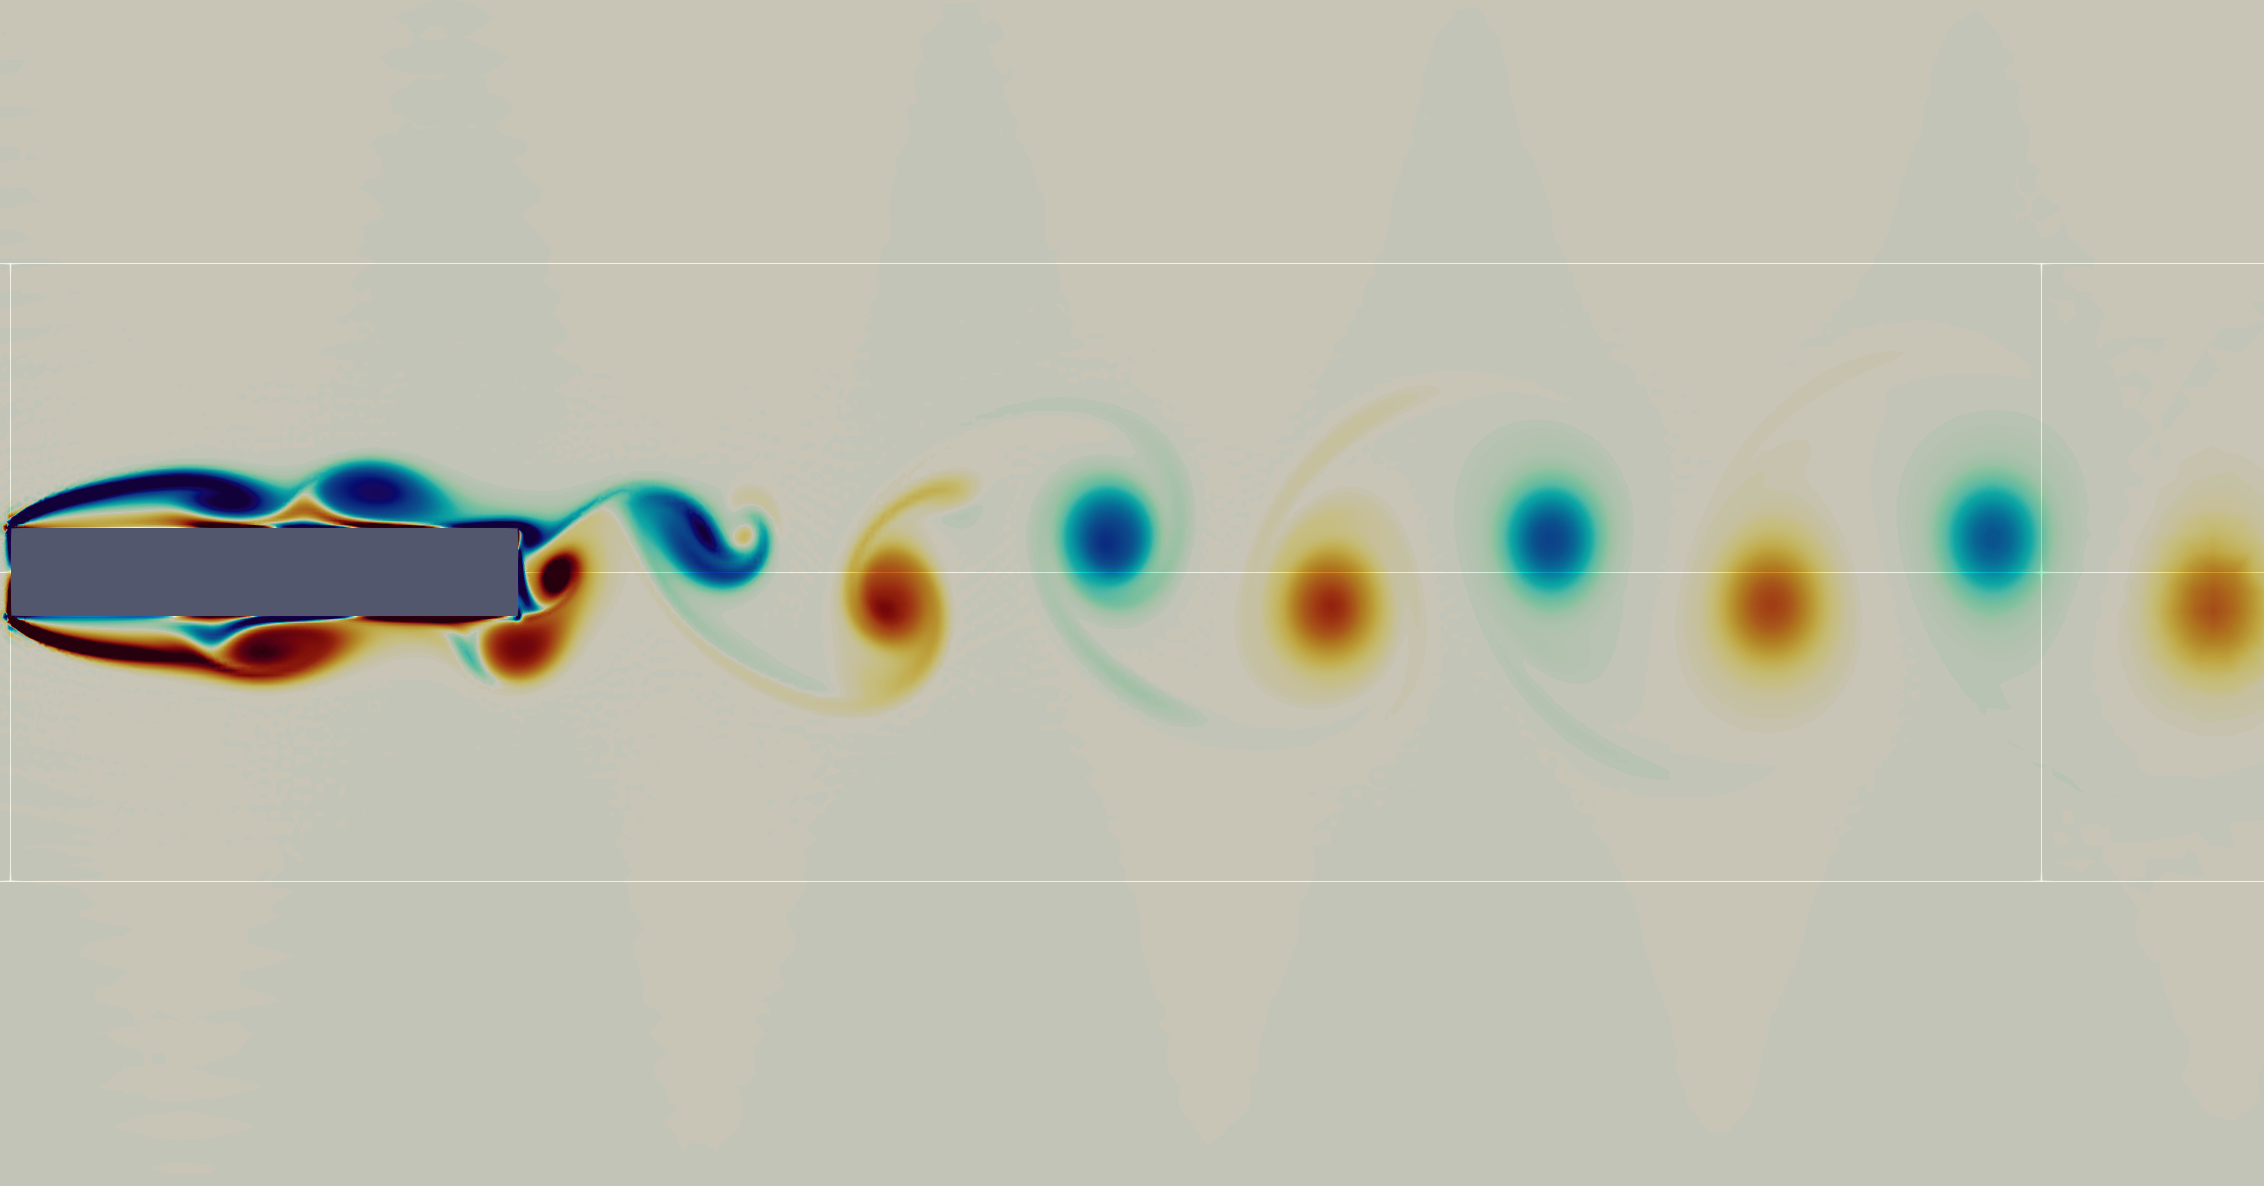
\includegraphics[width=0.49\textwidth]{./fig/AR5p75/vort_bf_Re550_100.png}
  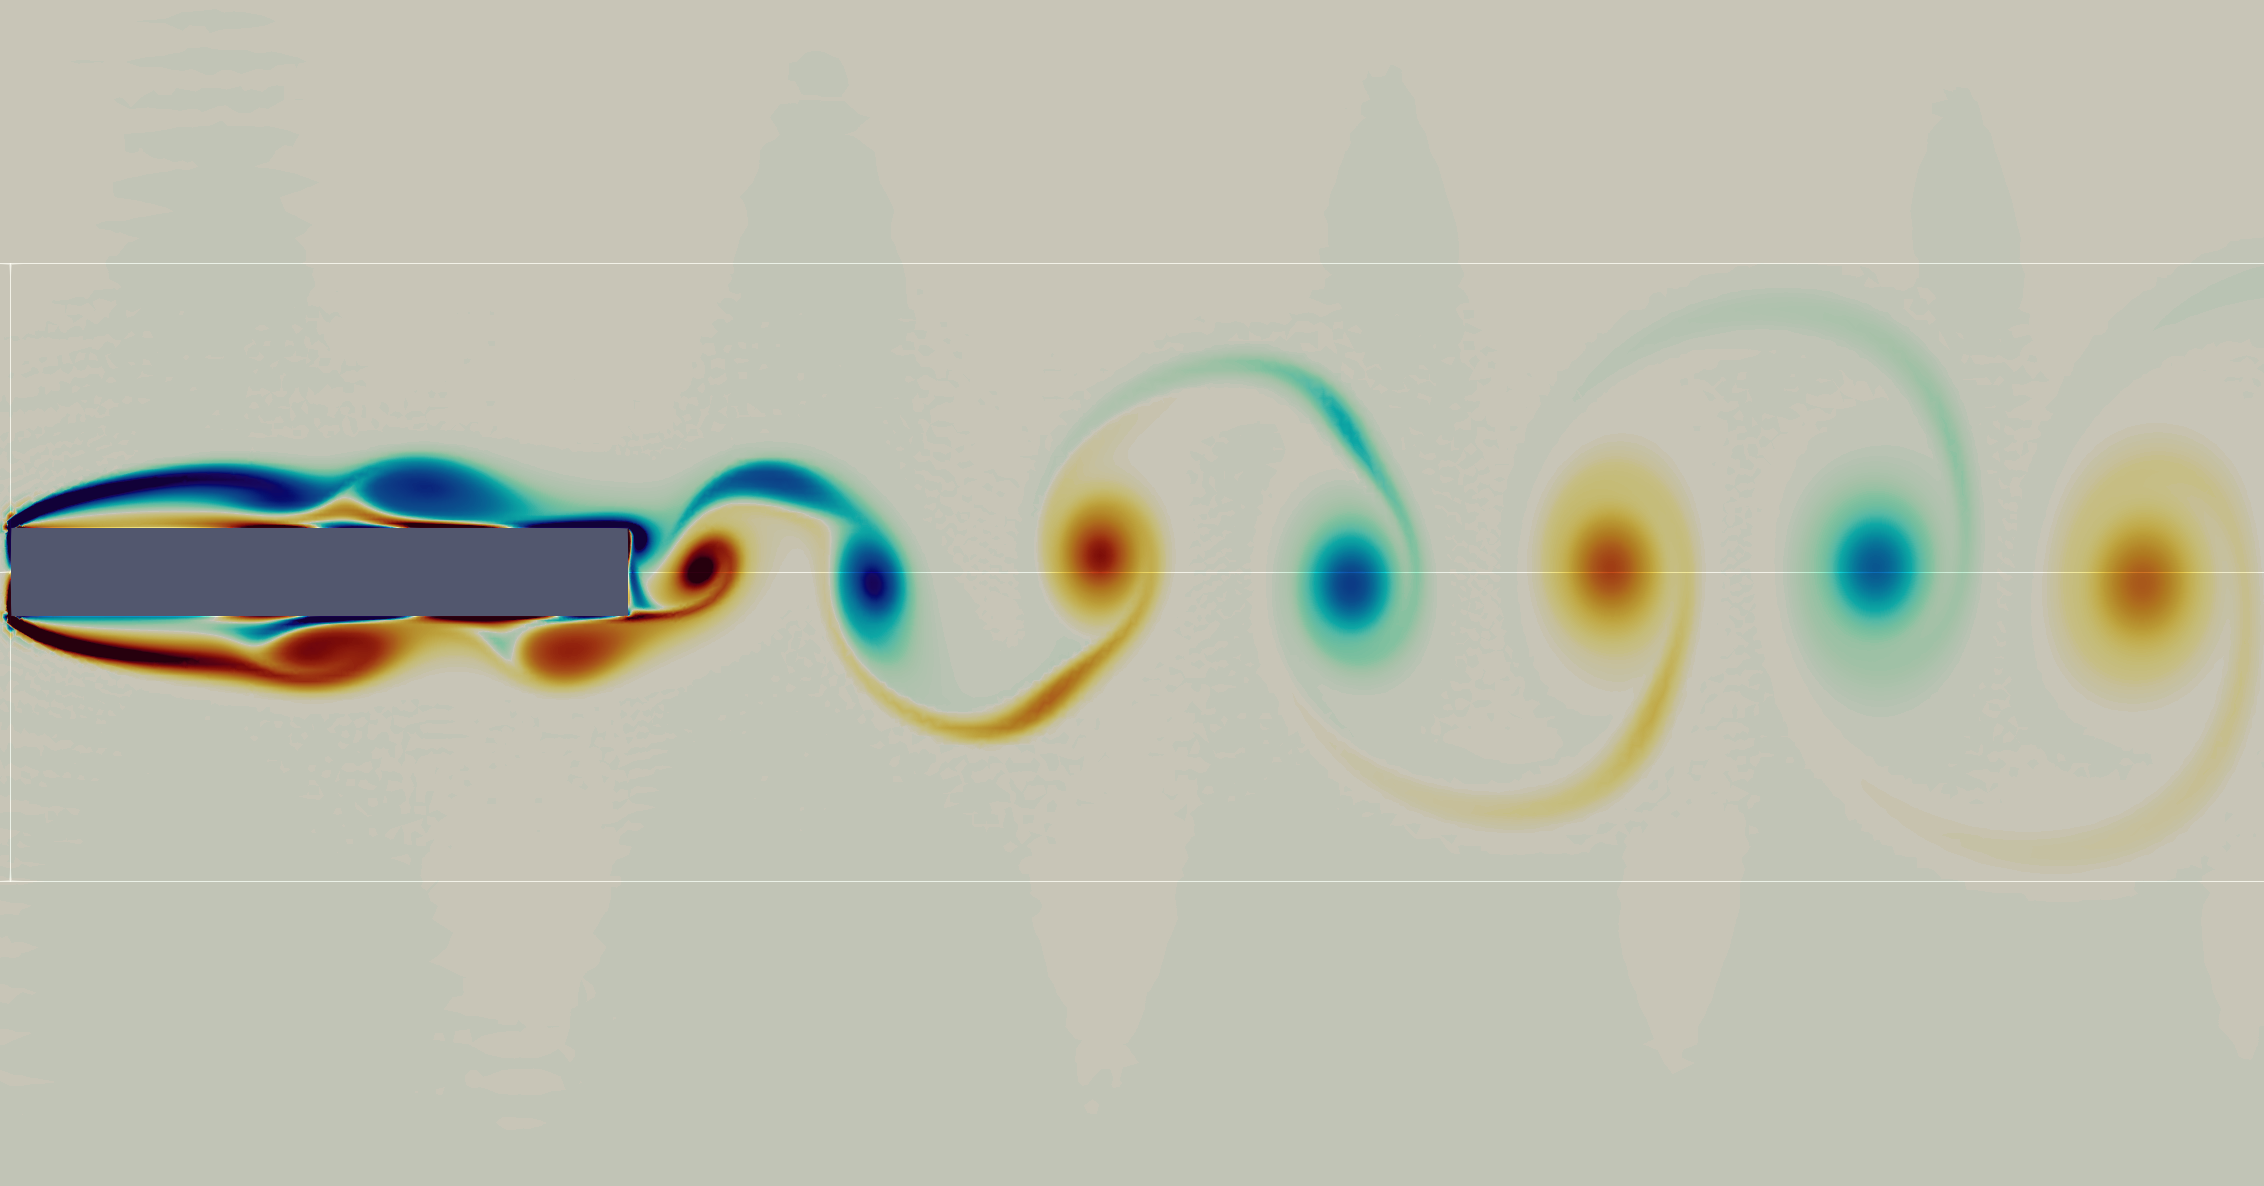
\includegraphics[width=0.49\textwidth]{./fig/AR7s/vort_bf_Re500_100.png}
  \caption{Instantaneous visualisations of the 2D base-flow for $\AR=5.75$ at $Re=550$ (left) and $\AR=7$ at $Re=500$ (right). The blue-to-red colour is for spanwise vorticity in the $-5 \le \Omega_z \le 5$ range. For $\AR=5.5$ the flow is dominated by the TE vortex shedding dynamics. When a LE crosses the TE, it merges with the new generating TE vortex from the same side. For $\AR=7$ the flow is domianted by the LE vortex shedding due to the different phase of the LE and TE vortex shedding. When a LE vortex crosses the TE, a new TE vortex is shed from the opposite side.}
  \label{fig:bf_elongated}
\end{figure}

The interaction between the LE and TE vortices in the $n=2$ LE-dominated regime closely resembles the behaviour observed in the $n=1$ case (see figure~\ref{fig:snap_ar4_ar4p5}a,b). This similarity is illustrated in figure~\ref{fig:bf_elongated}a, which presents a representative case at $\AR = 5.75$ and $Re = 550$.

For completeness, we now briefly discuss the $n=2$ and $n=3$ TE-dominated regimes. Figure~\ref{fig:bf_elongated}b shows a representative instantaneous visualisation of the $n=2$ LE-dominated regime at $\AR = 7$ and $Re = 500$. The observed behaviour is analogous to that in the $n=3$ LE-dominated regime at $\AR = 9$. A detailed characterisation of these regimes can be found in \citet{chiarini-quadrio-auteri-2022}.
%
In these TE-dominated regimes, the wake dynamics near the trailing edge closely resemble those of a streamlined elongated cylinder, with no observable separation from the leading edge \citep{chiarini-quadrio-auteri-2022}. The vortex shedding process is primarily governed by the TE dynamics, with LE vortices playing a negligible role. Upon reaching the TE corner, indeed, LE vortices merge into the developing recirculation region at the base of the cylinder, without significantly perturbing the formation or shedding of the subsequent TE vortex. Figure~\ref{fig:bf_elongated} clearly illustrates the merging of the positively signed LE and TE vortices near the lower corner of the trailing edge.

\begin{figure}
  \centering
  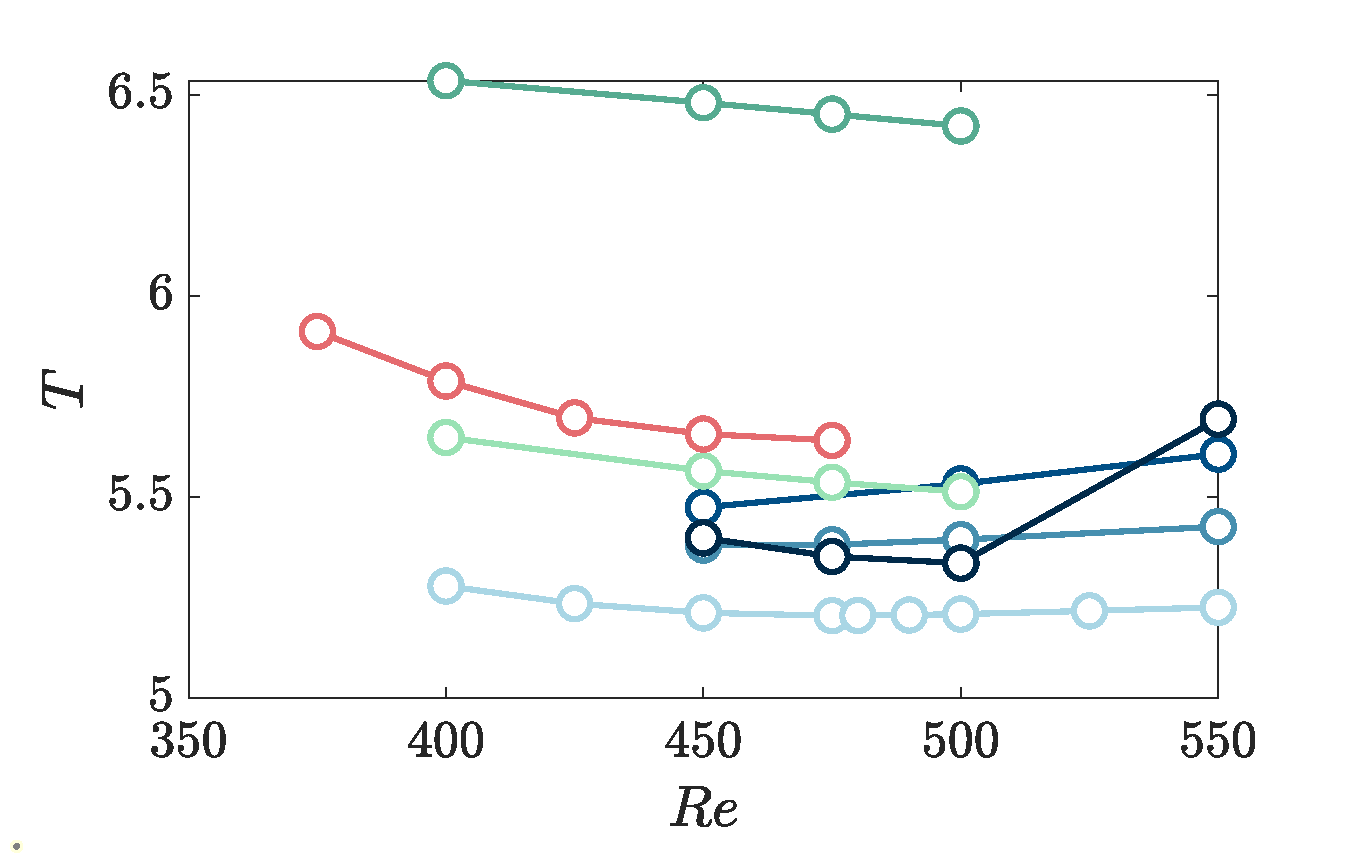
\includegraphics[width=0.49\textwidth]{./fig/long/T_Re.eps}
  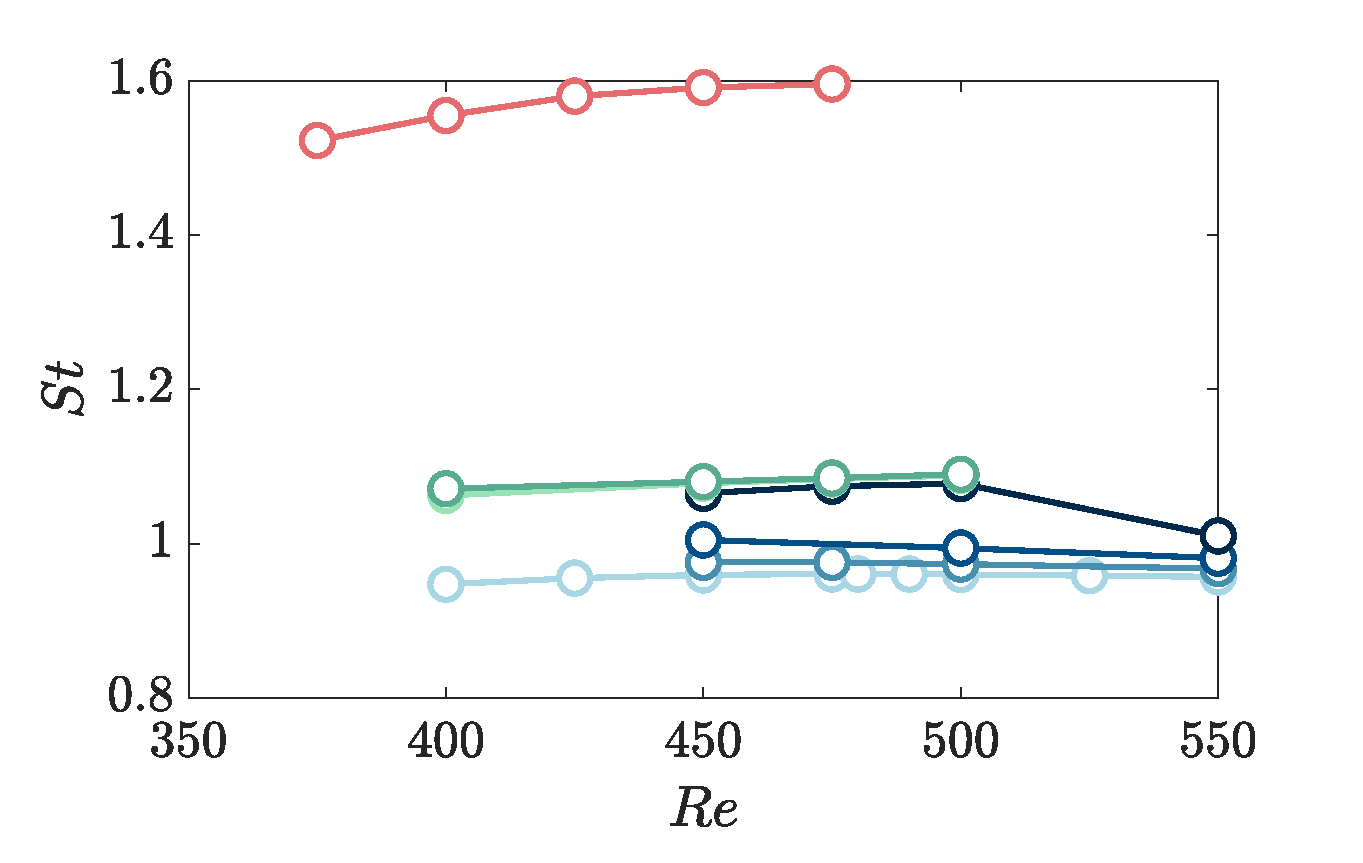
\includegraphics[width=0.49\textwidth]{./fig/long/St_Re.eps}
  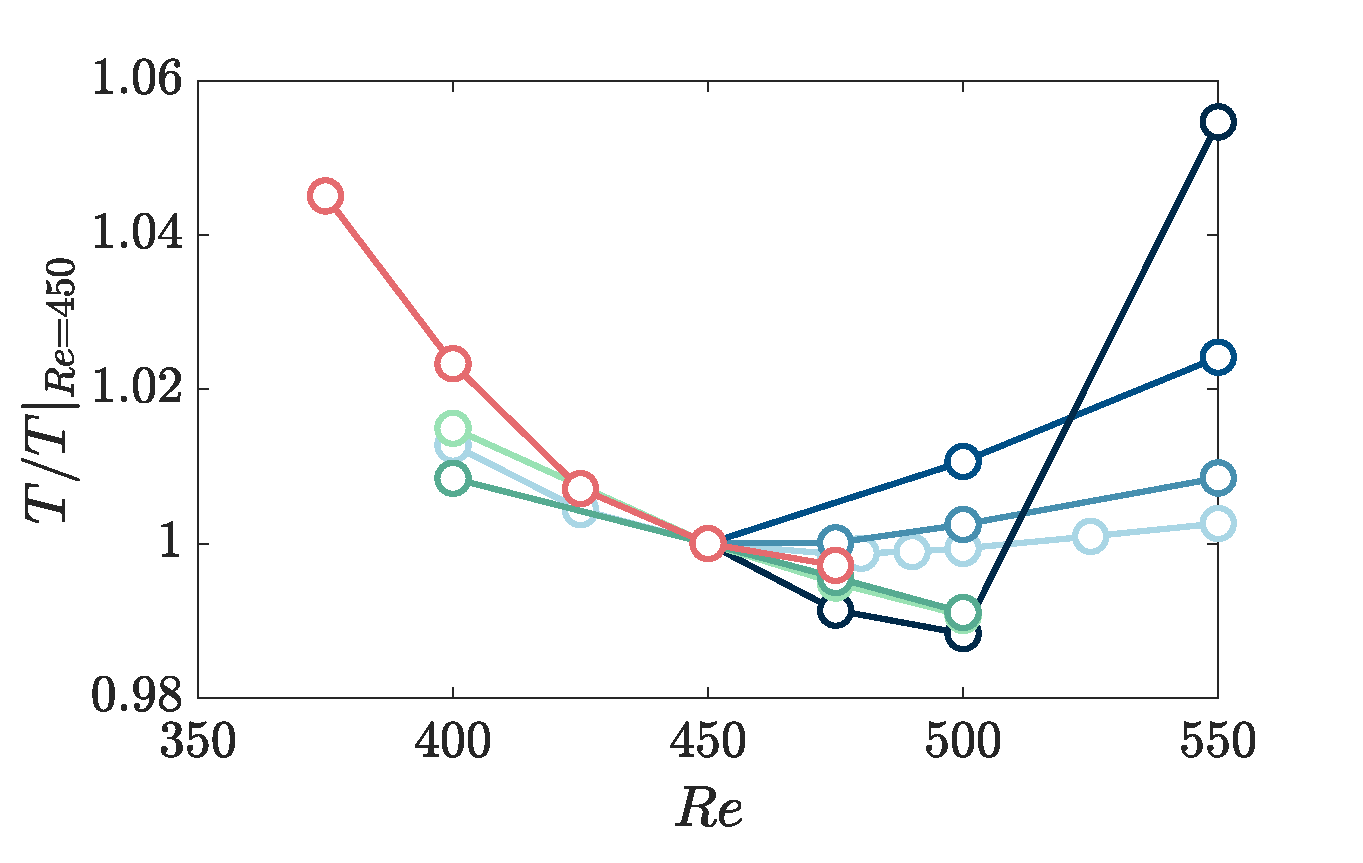
\includegraphics[width=0.49\textwidth]{./fig/long/T_Re_b.eps}
  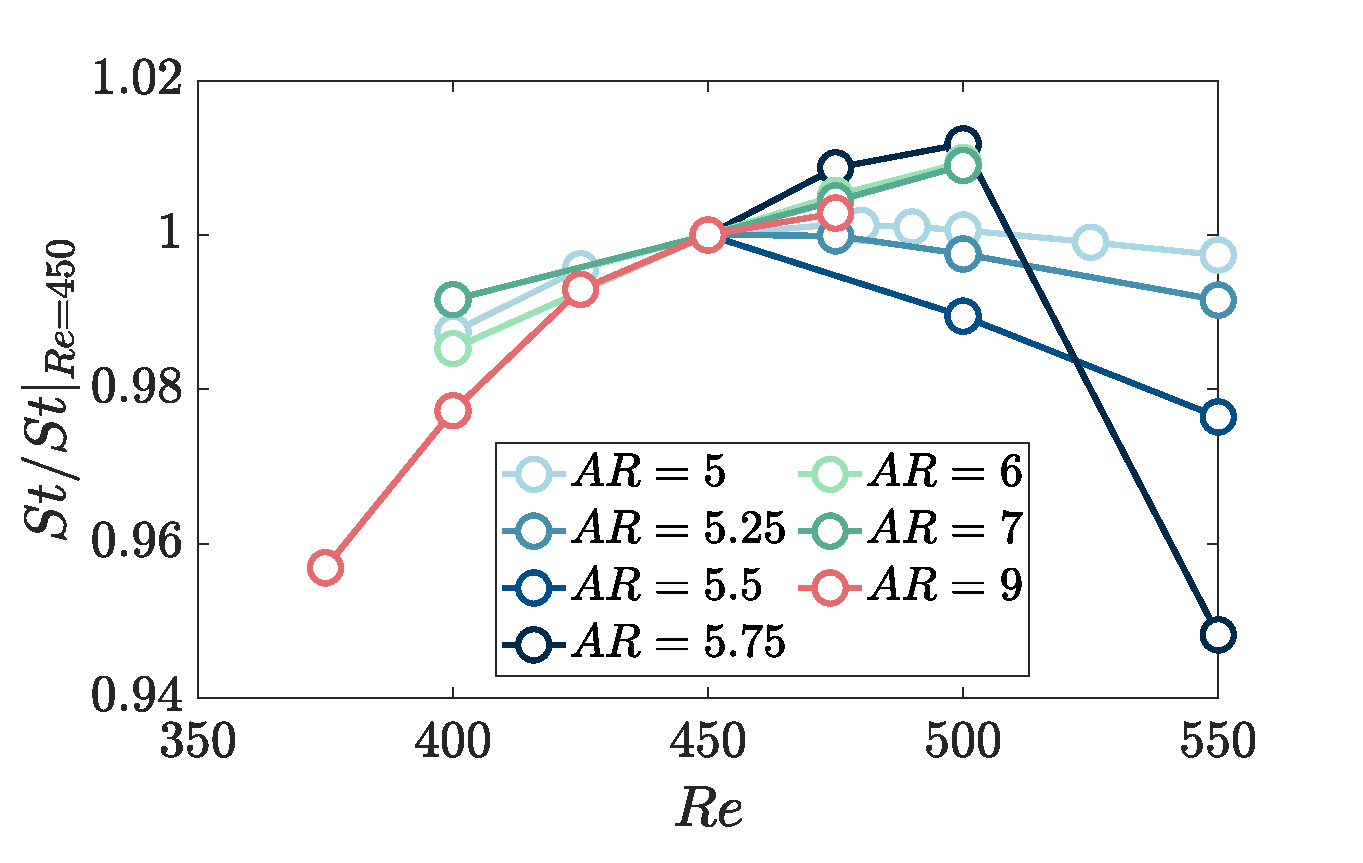
\includegraphics[width=0.49\textwidth]{./fig/long/St_Re_b.eps}
  \caption{xx}
  \label{fig:T_St_Re_long}
\end{figure}

This behaviour is further illustrated in figure \ref{fig:T_St_Re_long}, which shows the variation of the shedding period with Reynolds number for $5 \le \AR \le 7$ and $\AR = 9$. Different flow regimes are distinguished by colour: blue and red correspond to the $n = 2$ and $n = 3$ regimes dominated by TE vortex shedding, while green identifies the $n = 2$ regime governed by LE vortex shedding. As expected, within the considered $Re$ range, the Strouhal number $St_L$, increases approximately linearly with $\AR$ for $5 \le \AR \le 5.75$ (corresponding to the oblique $n = 2$ branch), and then collapses to a nearly constant value close to 1.1 for $6 \le \AR \le 7$ (the horizontal $n = 2$ branch).
%
Across all aspect ratios examined, the shedding period exhibits only a weak dependence on $Re$, though this sensitivity increases slightly with $\AR$. Notably, the period $T$ shows a non-monotonic dependence on $\AR$: it decreases at lower $Re$, but increases with $\AR$ at higher $Re$.


\subsection{The unstable modes}

\begin{figure}
  \centering
  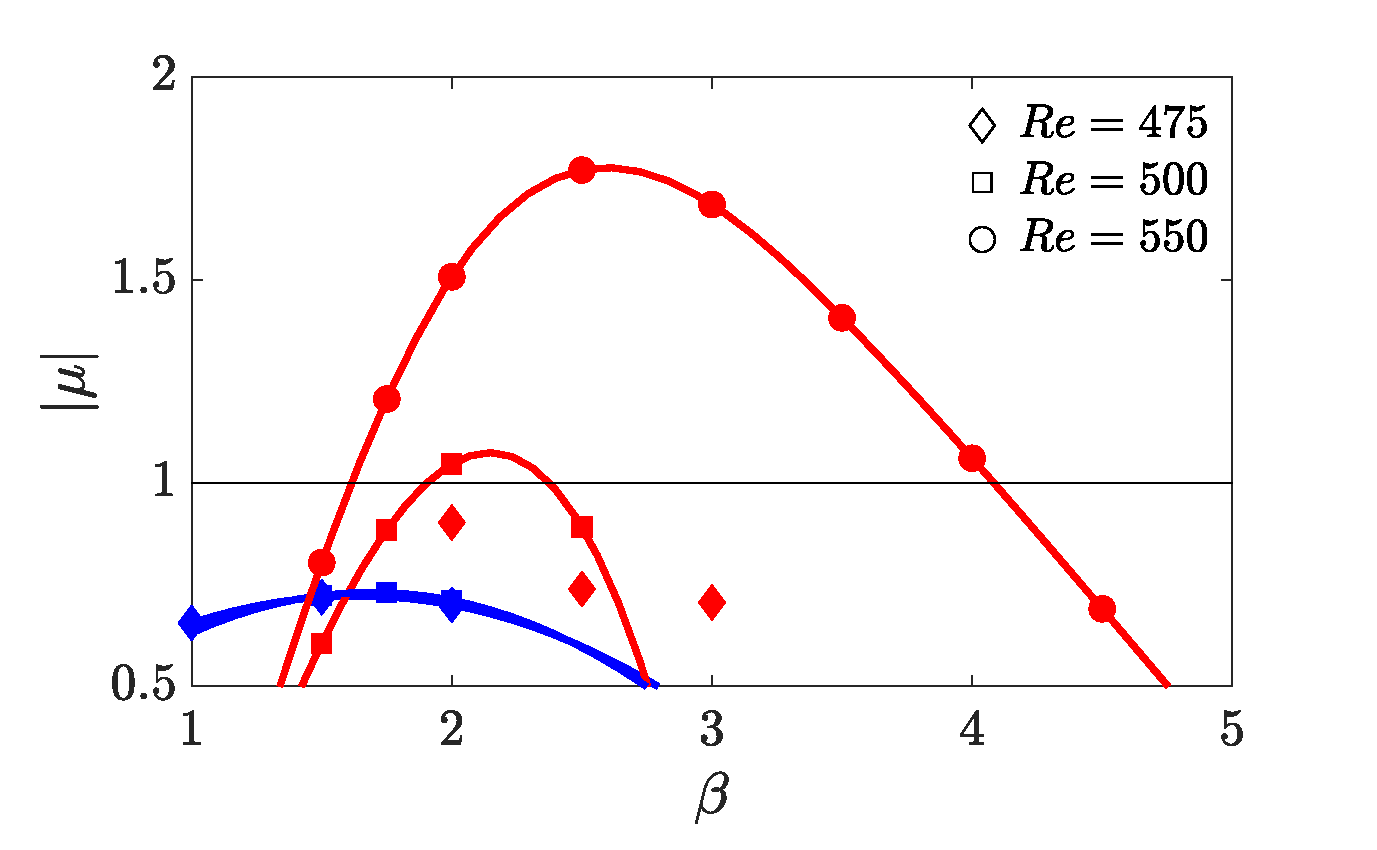
\includegraphics[width=0.49\textwidth]{./fig/AR5s/multipliers_AR5p25.eps}  
  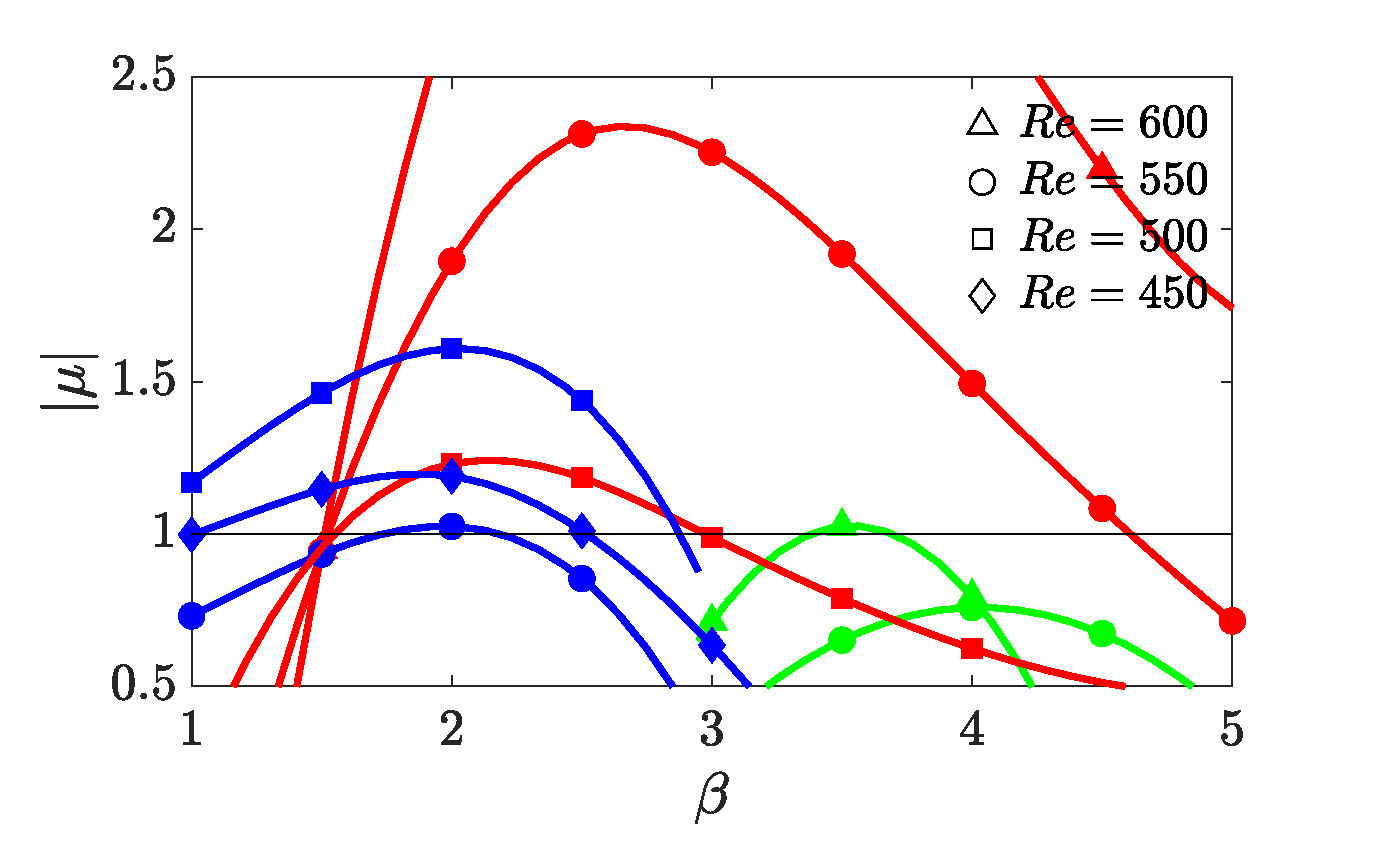
\includegraphics[width=0.49\textwidth]{./fig/AR5s/multipliers_AR5p5.eps}  
  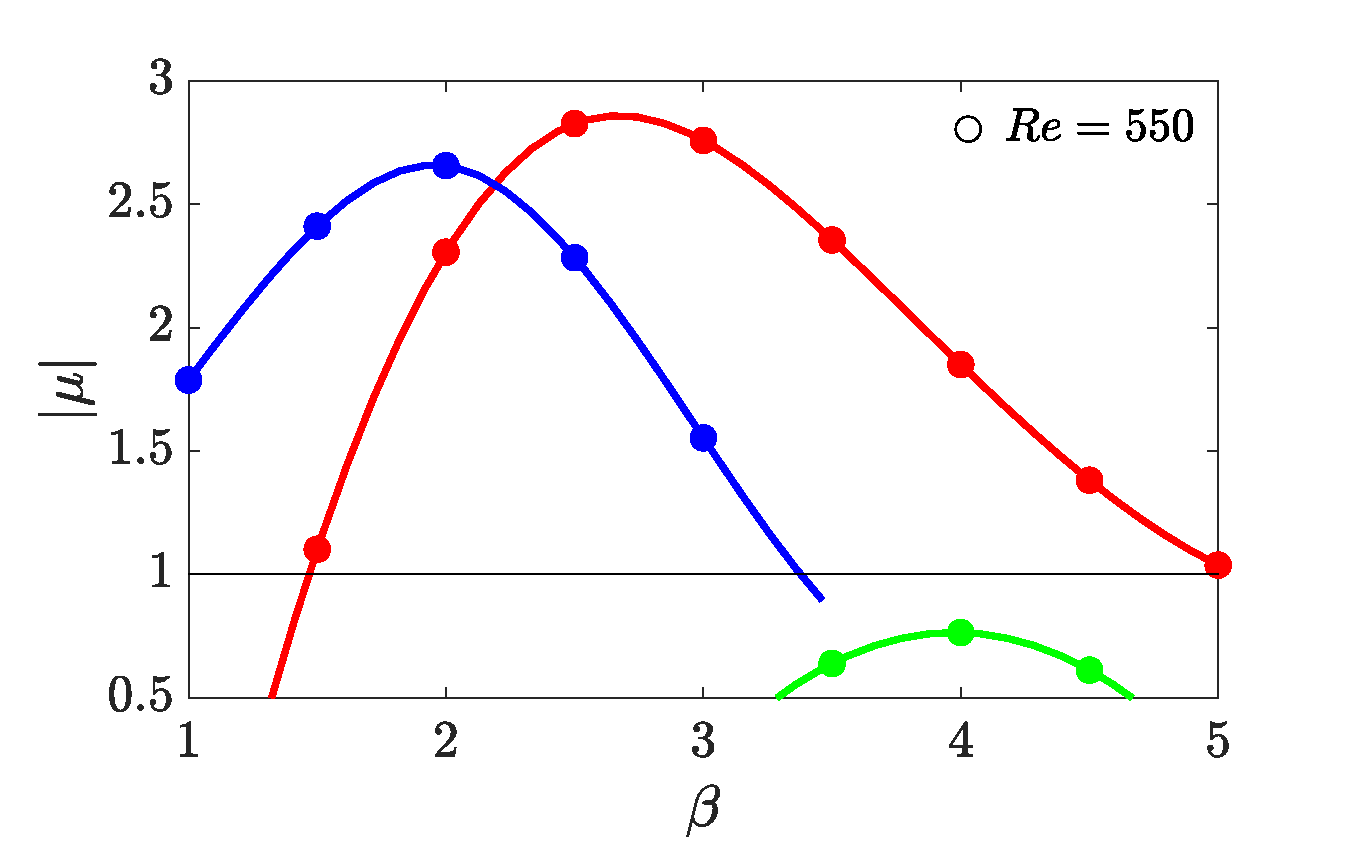
\includegraphics[width=0.49\textwidth]{./fig/AR5s/multipliers_AR5p75.eps} 
  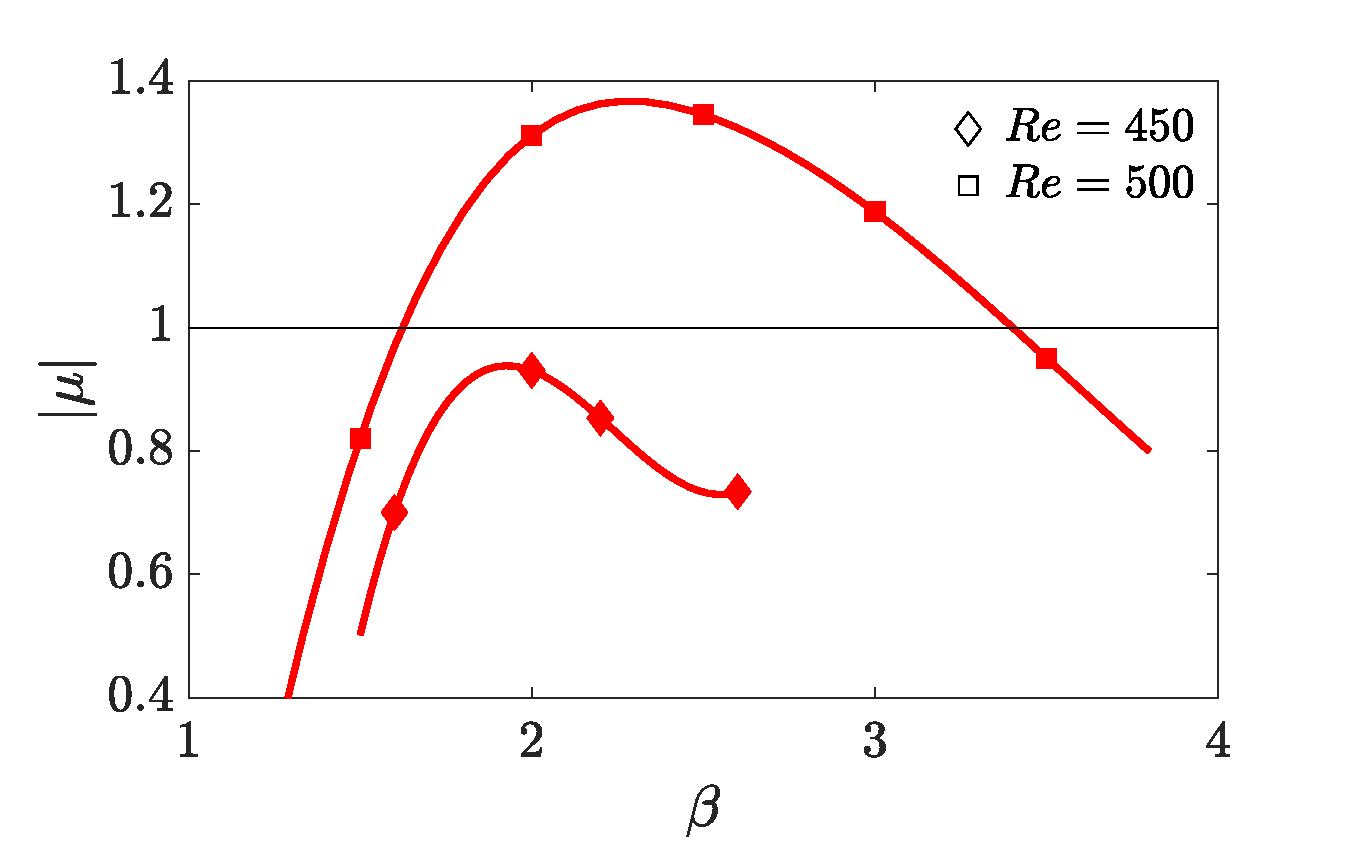
\includegraphics[width=0.49\textwidth]{./fig/AR7s/multipliers_AR6.eps}  
  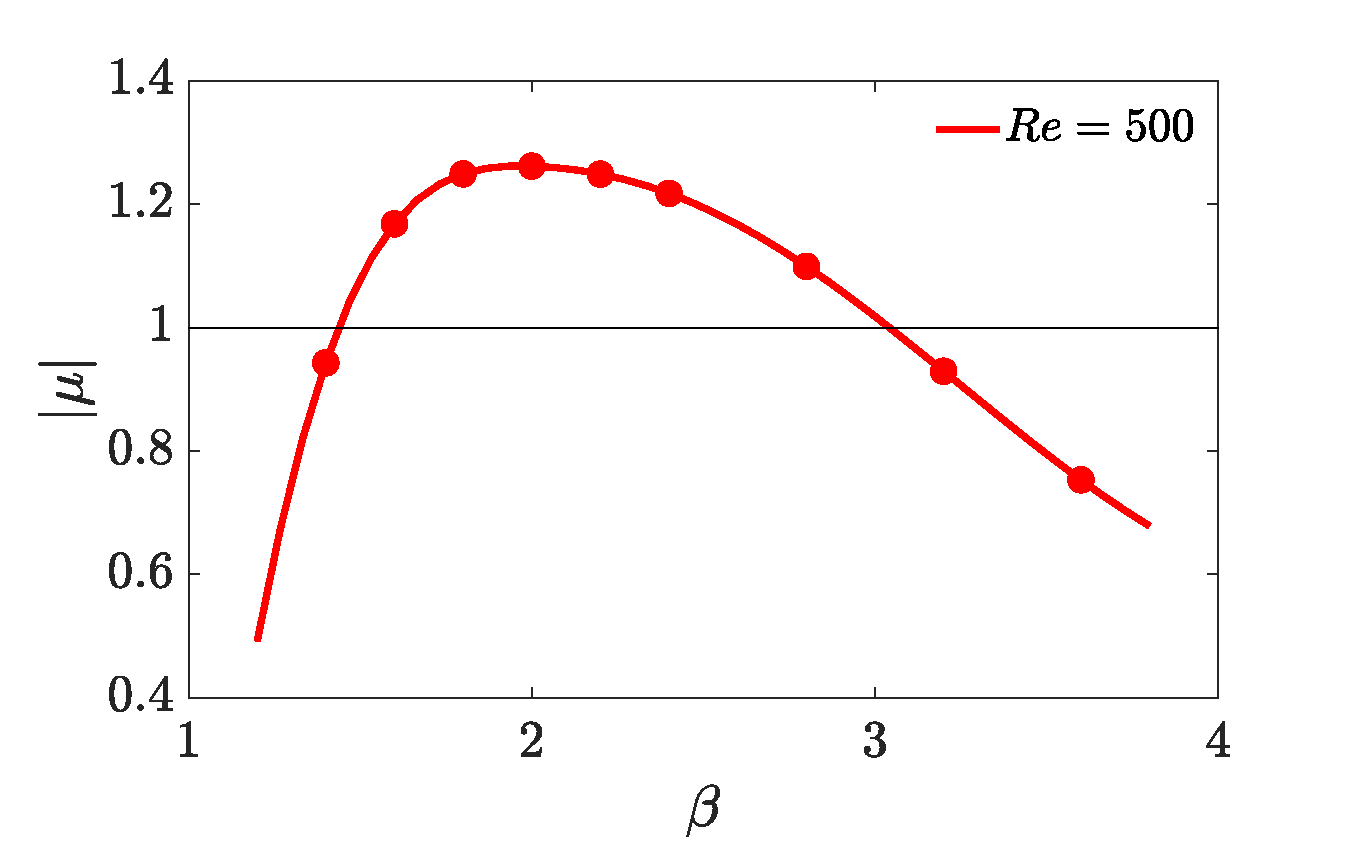
\includegraphics[width=0.49\textwidth]{./fig/AR7s/multipliers_AR7.eps}
  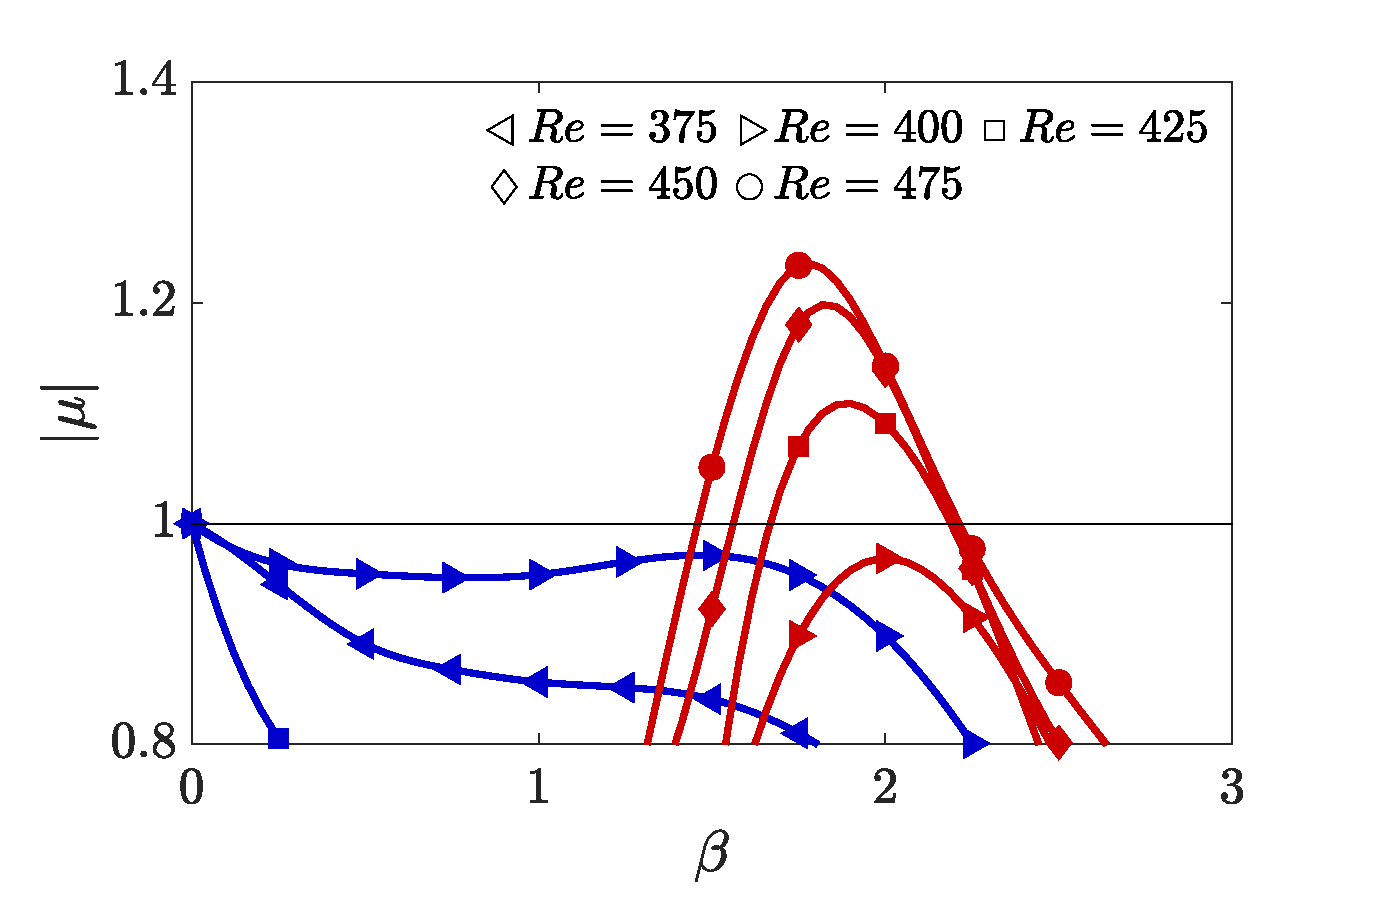
\includegraphics[width=0.49\textwidth]{./fig/AR9s/multipliers.eps}
  \caption{XX ADD THE UNSTABLE MULTIPLIERS USING $\AR=5.5$ and different $\beta$ and $Re$ to show XX}
  \label{fig:multipliers_long}
\end{figure}

\begin{figure}
  \centering
  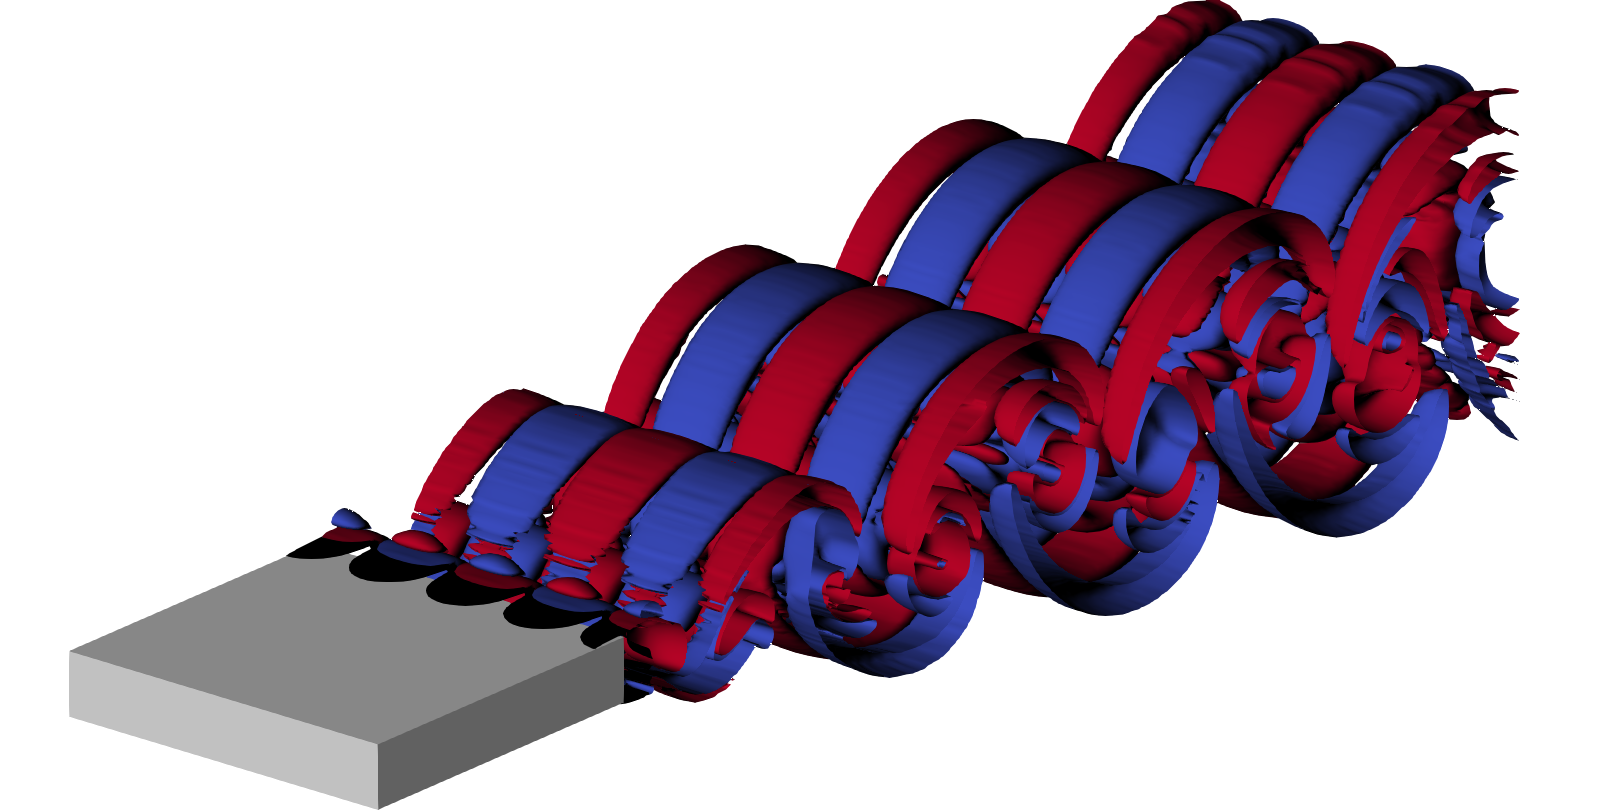
\includegraphics[width=0.49\textwidth]{./fig/AR5s/Floqetmode_beta_2_Re550_AR5p5_A.png}
  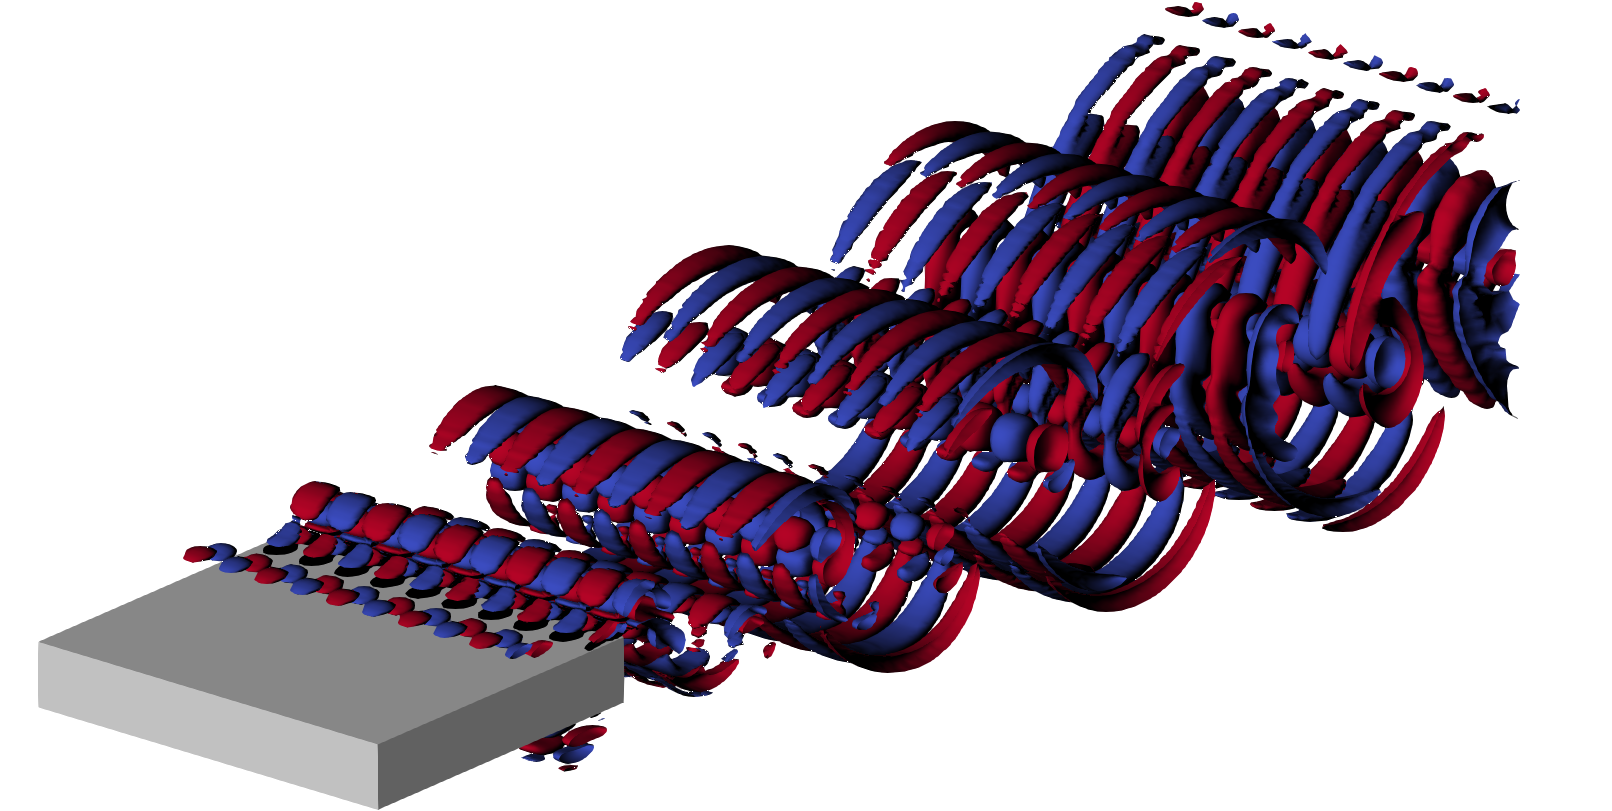
\includegraphics[width=0.49\textwidth]{./fig/AR5s/Floqetmode_beta_4p75_Re550_AR5p5_Ap.png}
  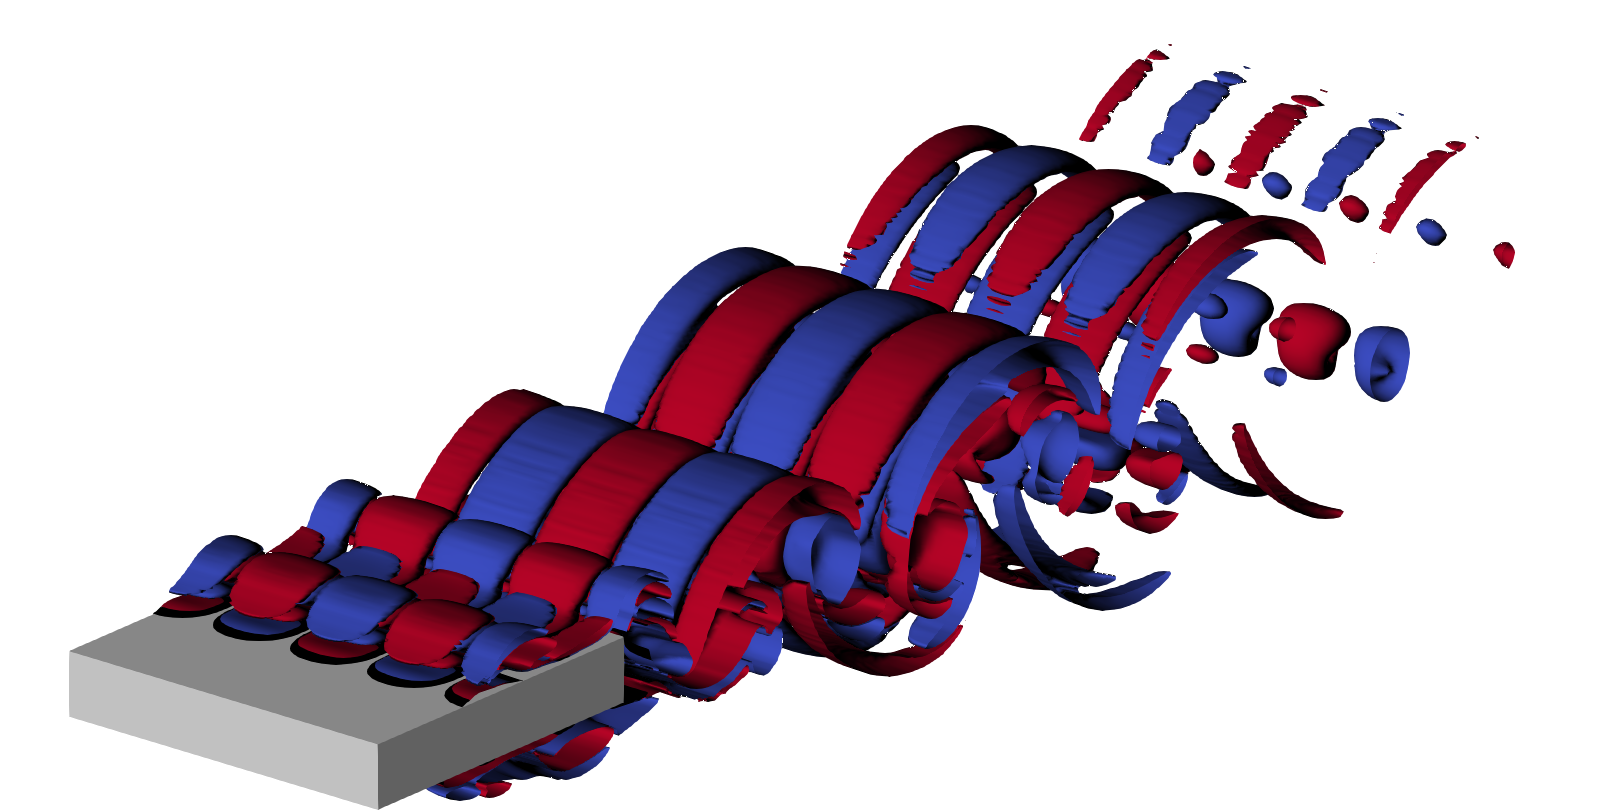
\includegraphics[width=0.49\textwidth]{./fig/AR5s/Floqetmode_beta_2_Re550_AR5p5_QS.png}   
  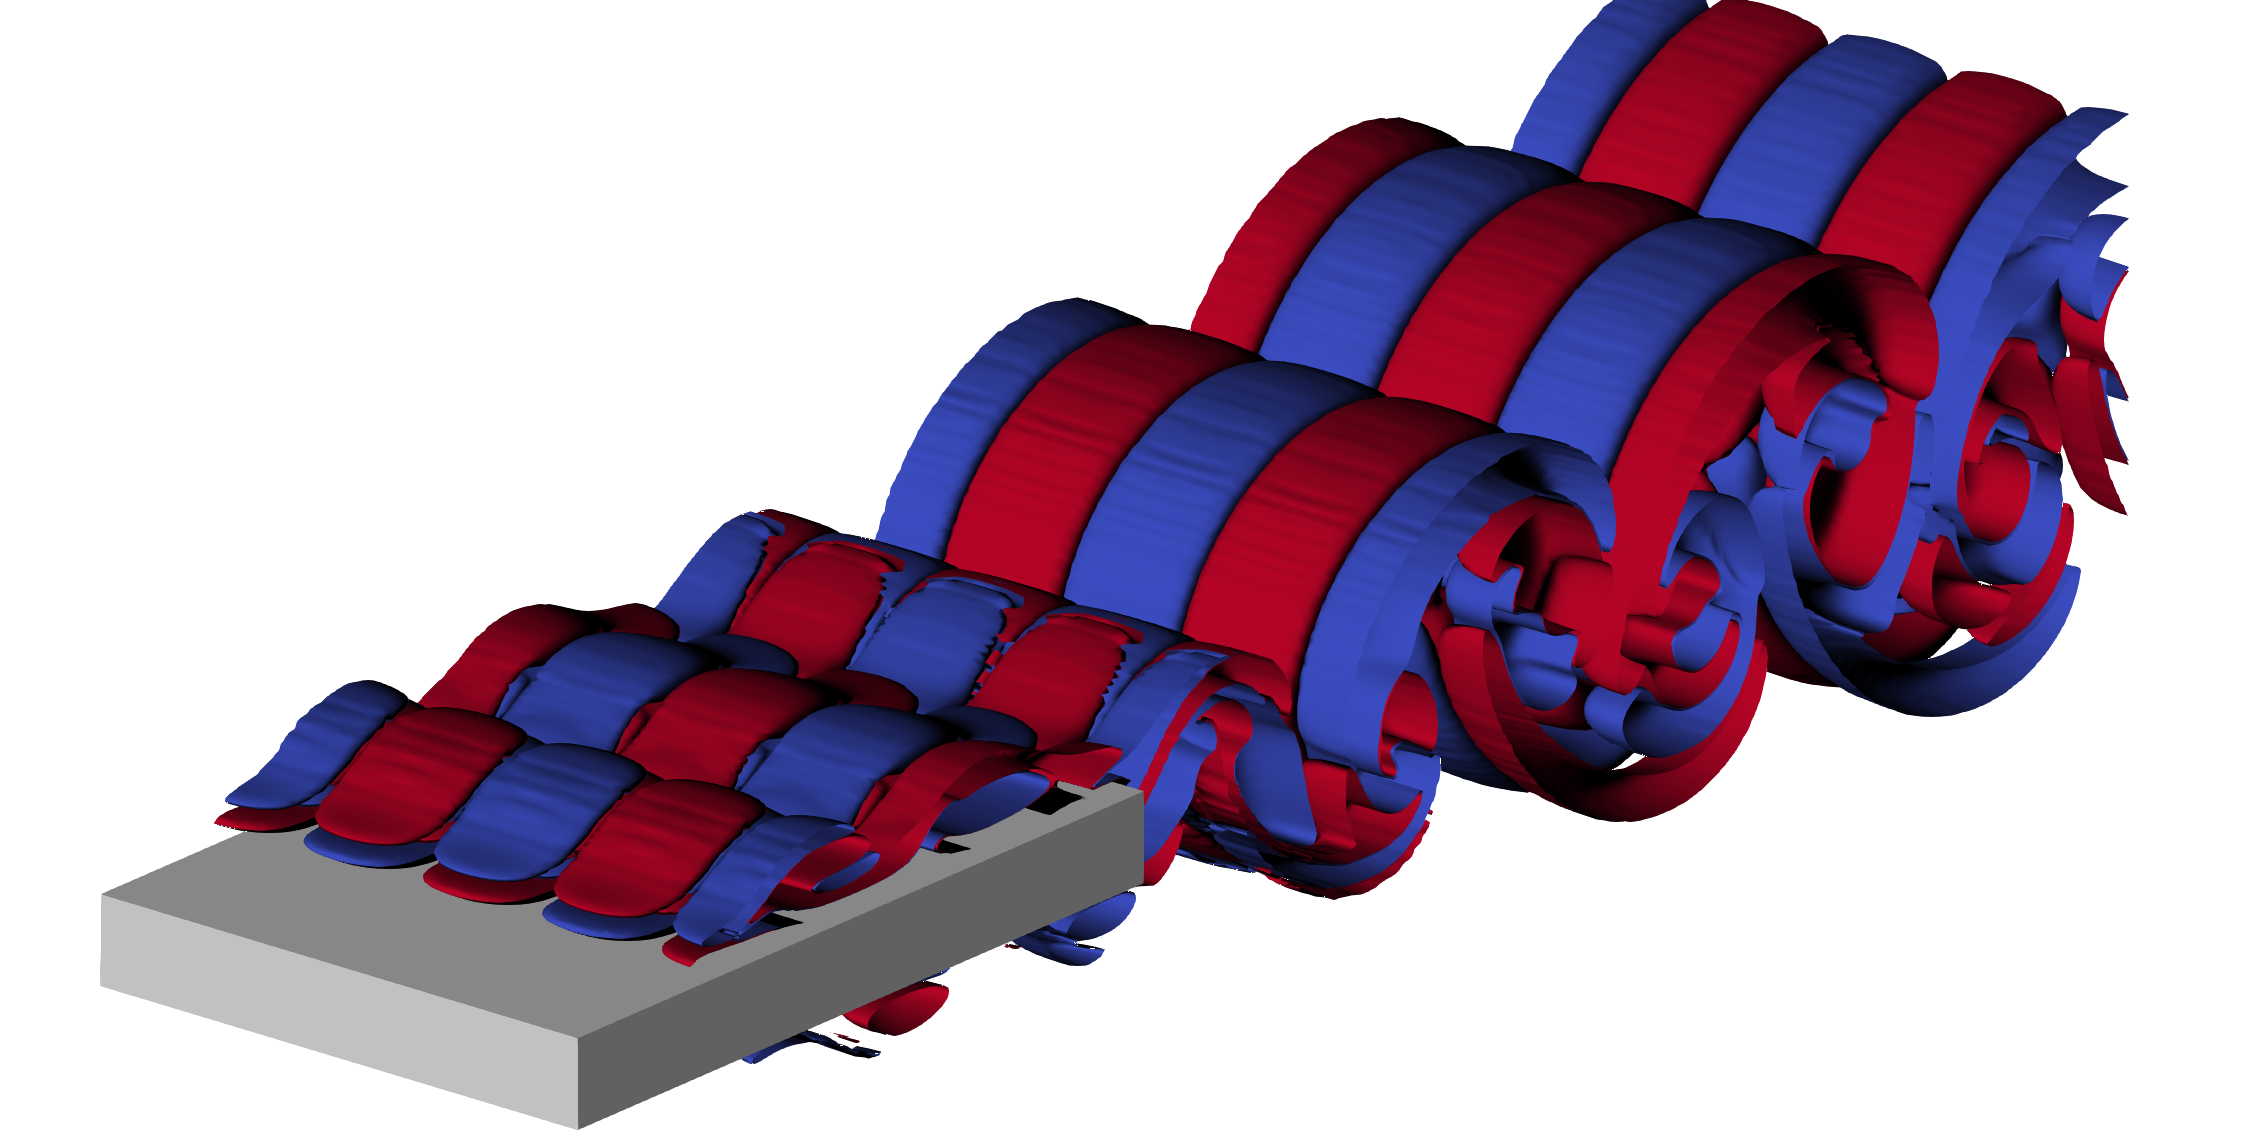
\includegraphics[width=0.49\textwidth]{./fig/AR9s/Floquet_AR9_Re450_beta2_modeQS.png}
  \caption{Three-dimensional reconstruction of the unstable modes for elongated bodies.}
  \label{fig:modes_long}
\end{figure}

Figure \ref{fig:multipliers_long} presents the leading Floquet multipliers for $5.25 \le \AR \le 9$ over a range of Reynolds numbers, marking the onset of the 3D instabilities. The spatial structures of the corresponding unstable modes are shown in figure \ref{fig:modes_long}. The bifurcation scenario changes markedly with $\AR$, reflecting variations in the topology of the base flow. As discussed below, two distinct wake modes become unstable at aspect ratios where TE vortex shedding dominates the base flow. These modes do not appear when the flow is instead governed by LE vortices. However, across all $\AR$ values considered, the so-called $QS$ mode---associated with LE vortex dynamics---becomes unstable. The sequence and nature of the bifurcations are therefore strongly dependent on $\AR$. Note that for $\AR = 5.75$, results are presented only for $Re = 550$, as lower Reynolds numbers exhibit a loss of near-wake periodicity due to a convective instability (see \S\ref{sec:farwake}).

Figure \ref{fig:multipliers_long} shows that, for all aspect ratios considered, a branch of Floquet multipliers centered around $\beta \approx 2.1$ crosses the unit circle in the complex plane. This branch comprises a pair of complex-conjugate multipliers with negative real parts and very small imaginary components (see figure \ref{}), indicating that the 2D base flow becomes unstable to weakly subharmonic, 3D perturbations in elongated configurations ($\AR \ge 5$). This instability, referred to as mode $QS$, is not linked to wake dynamics. Instead, it arises from an inviscid interaction involving the LE vortices simultaneously accommodated along the lateral surfaces of the cylinder; see \cite{chiarini-quadrio-auteri-2022d} for further details.
%
The perturbation field is concentrated along the lateral surfaces and is non-negligible near the $n=2$ and $n=3$ LE vortices for $5 \le \AR \le 7$ and $\AR=9$, respectively (see bottom panels of figure \ref{fig:modes_long}).

A similar instability was reported by \cite{chaurasia-thompson-2011}, who studied the flow past a square flat plate in the limit $L\rightarrow \infty$. There, the instability was associated with vortices shed from the LE shear layer and was found to be purely subharmonic---characterised by a single, real negative Floquet multiplier crossing the unit circle. This is consistent with the theoretical analysis of \cite{marques-lopez-blackburn-2004}, which showed that subharmonic bifurcations are prohibited in base flows with exact spatio-temporal symmetry. However, when this symmetry is broken---due, for example, to the absence of a trailing edge or slight asymmetries in the base flow---subharmonic bifurcations become admissible.

The presence of mode QS highlights a fundamental distinction in the bifurcation pathway to turbulence between flows past sharp-edged rectangular bodies and those past elongated geometries with smooth leading edges. In the latter case, secondary instabilities are predominantly governed by wake dynamics, with the sequence and nature of bifurcations varying systematically with $\AR$ \citep{ryan-thompson-hourigan-2005}. In contrast, for the present geometry, the primary three-dimensional instability originates from inviscid interactions involving LE vortices, independent of the wake. This underscores the critical role of sharp-edged geometries in reshaping the instability landscape, enabling the emergence of modes driven by localised dynamics along the body’s lateral surfaces.

The critical Reynolds number associated with mode $QS$ exhibits a slight decreasing trend with increasing aspect ratio, from $Re_c \approx 475-500$ for $\AR=5.25$ to $Re_c \approx 400-425$ for $\AR=9$. 

For aspect ratios where the base flow is dominated by TE vortex shedding---specifically, $5 \le \AR \le 5.75$ and $\AR = 9$---two additional unstable modes are identified, both arising exclusively from wake dynamics. The first corresponds to a branch of real, positive Floquet multipliers centered around $\beta \approx 2$, consistent with the classical wake mode A observed in shorter bodies. This is the first mode to become unstable at intermediate $\AR$ within the TE-dominated regime, a behaviour that appears to depend on the relative phase between the LE and TE vortices. As shown in figure~\ref{fig:modes_long}, this mode is spatially confined to the near wake and exhibits the same spatio-temporal symmetries as previously reported (see \S\ref{sec:short}). When permitted, the critical Reynolds number associated with this mode decreases with increasing $\AR$, being $Re_c \lesssim 450$ for $\AR = 5.5$ and approximately $Re_c \approx 395$ for $\AR = 9$.
%
The second instability branch, also consisting of real, positive Floquet multipliers, emerges at $\AR = 5.5$ and $\AR = 5.75$, centred around $\beta \approx 3.5$–$4$. This mode, denoted as mode $A'$, shares the same spatio-temporal symmetries as mode $A$ but is characterised by a shorter spanwise wavelength. Like mode $A$, it is confined to the wake, with negligible support along the cylinder’s lateral surfaces, reinforcing its wake-driven nature. Mode $A'$ is not observed at $\AR = 5.25$ or $\AR = 9$ within the considered Reynolds number range, and constitutes the second or third unstable mode depending on $\AR$. As with mode $A$, its emergence is contingent on the presence of natural TE shedding; when the base flow is dominated by LE vortex dynamics, mode $A'$ remains suppressed.

%\subsection{The physical mechanism of mode $A$}

%Within the Reynolds number range considered, mode A remains stable for $5 \le \AR \le 5.25$, becomes unstable for $5.5 \le \AR \le 5.75$, and is marginally stable at $\AR = 9$. Notably, for $\AR = 5.5$ and $5.75$, mode $A$ is the first to destabilise and is responsible for initiating the transition to three-dimensionality. In this range, and increase of $\AR$ destabilises mode $A$. This is confirmed by nonlinear 3D simulations, as discussed later.

%For rectangular cylinders, mode A reappears intermittently as $\AR$ increases. Its presence is closely linked to the phasing of the vortex shedding: when natural TE shedding is permitted by the base flow, mode A emerges and governs the three-dimensional transition. Conversely, when TE shedding is suppressed by the passage of LE vortices, the mechanism sustaining mode A is inhibited, and the transition is instead driven by mode QS.

\begin{figure}
  \centering
  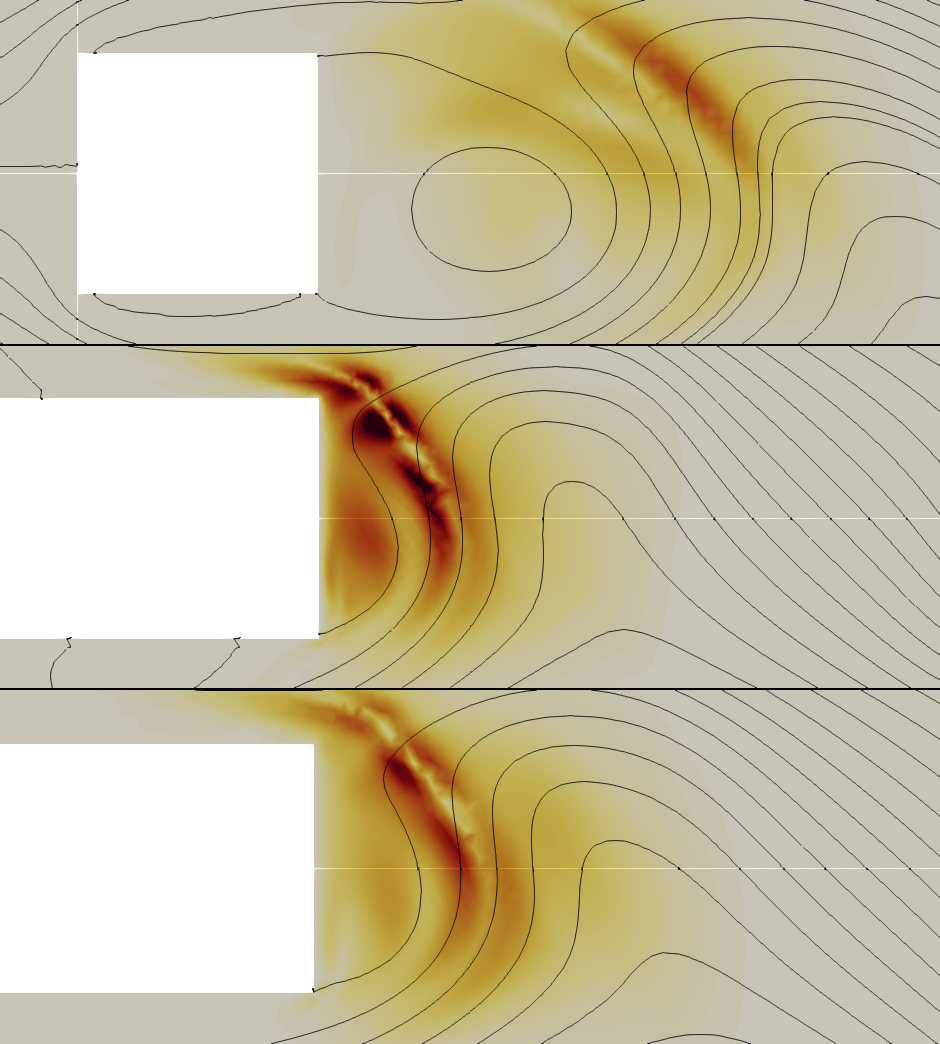
\includegraphics[width=0.49\textwidth]{./fig/AR5p5/sens_1-200-1p25_5p5-500-2_9-395_1p5_modeA_75.png}
  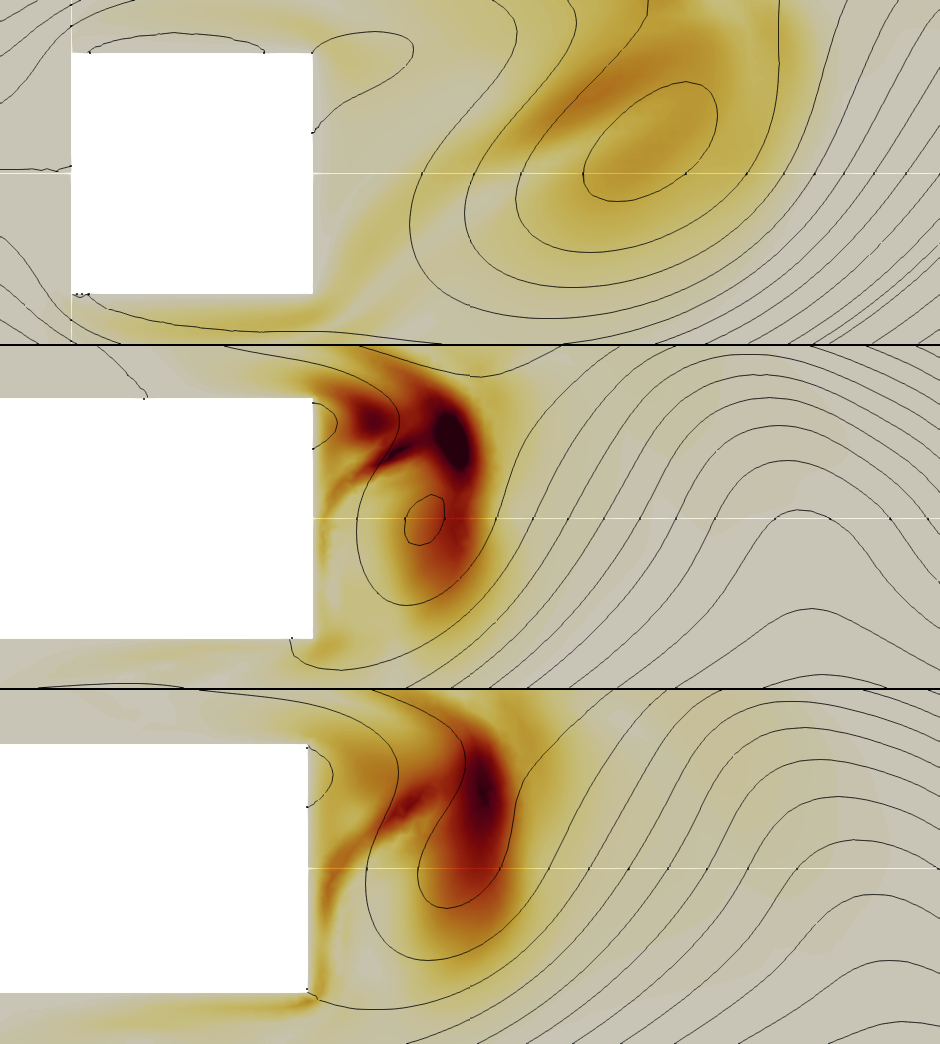
\includegraphics[width=0.49\textwidth]{./fig/AR5p5/sens_1-200-1p25_5p5-500-2_9-395_1p5_modeA_100.png}
  \caption{Structural sensitivity for mode A at two different instants within the shedding period. Comparison between $\AR=1$ at $Re=200$ and $\beta=1.25$, $\AR=5.5$ at $Re=500$ and $\beta=2$, $\AR=9$ at $Re=395$ and $\beta=1.5$. For $\AR=5.5$ the base flow is governed by the TE vortex shedding. Though, the characteristic lengths of the wake vortex are rather different the topology of the structural sensitivity resembles in both cases at the two phases. This further suggests that in both cases the two unstable modes coincide.}
  \label{fig:sens_modeA}
\end{figure}
%
To further demonstrate that the same mode $A$ emerges across different aspect ratios $\AR$ when TE vortex shedding is permitted, figure~\ref{fig:sens_modeA} shows the norm of the instantaneous structural sensitivity $I$ for three representative cases: $\AR = 1$, $Re = 200$, $\beta = 1.25$; $\AR = 5.5$, $Re = 500$, $\beta = 2$; and $\AR = 9$, $Re = 395$, $\beta = 1.5$. For each configuration, two distinct phases of the unsteady flow are examined. Across all cases, the spatial structure of the sensitivity field remains essentially unchanged and closely resembles that reported by \cite{giannetti-camarri-luchini-2010} for the canonical flow past a circular cylinder. The primary differences arise from variations in the size and topology of the base-flow streamlines.
%
Regions of significant sensitivity are consistently located between the clockwise and counter-clockwise vorticity layers originating from the lower and upper shear layers, respectively. In some cases, the sensitive region extends toward the TE corners where separation occurs. Notably, the structural sensitivity remains negligible along the lateral surfaces of the body, reinforcing the interpretation that this mode corresponds to a global wake instability. This further confirms that, even for elongated bodies, the LE vortices do not play a direct role in triggering the instability.
%
Interestingly, the appearance or suppression of mode $A$ depending on the phasing between the LE and TE vortices provides new insight into the nature of the underlying instability mechanism. Indeed, despite extensive experimental, numerical, and theoretical investigations---primarily focused on the circular cylinder---the precise physical origin of this secondary instability remains an open question. Several mechanisms have been proposed, including elliptic instabilities of the vortex cores \citep{williamson-1996,leweke-williamson-1998} and centrifugal-type instabilities; a comprehensive discussion is provided by \citet{thompson-etal-2001}.
%
More recently, \cite{giannetti-2015} applied Lifshitz-Hameiri theory along special Lagrangian trajectories in the wake of a circular cylinder, predicting both synchronous and asynchronous instabilities associated with specific Lagrangian orbits. While this approach offers valuable physical insight, a quantitative match with global stability results has yet to be firmly established. Instead, \cite{aleksyuk-heil-2023} examined the growth and decay of perturbations associated with mode $A$, identifying a tilting mechanism that operates analogously to Biot-Savart induction as a central driver of the instability.
%
In light of these studies, the present results, showing that mode $A$ emerges only when TE vortex shedding occurs in conjunction with specific wake dynamics, may offer valuable clues toward a deeper understanding of the transition to three-dimensionality, with potential implications even for the canonical circular-cylinder case.

In summary, for elongated bodies the onset of three-dimensionality is governed by either mode $QS$ or mode $A$, depending on $\AR$. When LE vortex shedding dominates, mode $QS$ is the first 3D mode to become unstable, with the transition driven by the inviscid interaction of LE vortices along the lateral surfaces of the cylinder. In contrast, when TE shedding dominates---and is permitted by the relative phase between LE and TE vortices---the first unstable mode is mode $A$, with three-dimensionality driven by wake dynamics, consistent with observations for shorter and more streamlined bodies. For rectangular cylinders, indeed, mode $A$ re-emerges intermittently as $\AR$ increases, with its presence being closely linked to the phasing of the LE and TE vortex shedding.

\subsection{On the amplification mechanism of modes $A$ and $QS$}

We now investigate the contributions of various physical mechanisms to the exponential growth of modes $A$ and $QS$ in the linear regime, specifically at the critical Reynolds number $Re = Re_{c2}$. Our analysis begins with the perturbation energy equation for the velocity field $\bm{u}$ (see equation~\eqref{eq:LNSEs}). Applying the Floquet ansatz \eqref{eq:ansatz}, we take the scalar product of the resulting equation with the complex conjugate velocity perturbation $\hat{\bm{u}}^*$, then add the complex conjugate of the same equation multiplied by $\hat{\bm{u}}$. After some algebraic manipulation and enforcing incompressibility, we derive an equation governing the time evolution of the perturbation energy density, $\hat{\bm{u}} \cdot \hat{\bm{u}}^*$, averaged over one shedding period, namely
%
\begin{equation}
  \begin{gathered}
  \frac{2 \Re(\sigma)}{T} \int_{t_0}^{t_0+T} \hat{u}_i \hat{u}_i^* \text{d}t = 
 \underbrace{-\frac{1}{T} \int_{t_0}^{t_0+T} \left( \hat{u}_j \hat{u}_i^* + \hat{u}_j^* \hat{u}_i \right) \frac{\partial U_i}{\partial x_j} \text{d} t}_{\mathcal{P}} +\\
 \underbrace{-\frac{1}{T} \int_{t_0}^{t_0+T} U_j \frac{\partial \hat{u}_i \hat{u}_i^*}{\partial x_j} \text{d} t }_{\mathcal{A}} + 
 \underbrace{-\frac{1}{T} \int_{t_0}^{t_0+T} \frac{\partial}{\partial x_i} \left( \hat{p} \hat{u}_i^* + \hat{p}^* \hat{u}_i \right) \text{d}t }_{\mathcal{T}_p}+ \\
\underbrace{ +\frac{1}{T} \int_{t_0}^{t_0+T} \frac{1}{Re} \left[ \frac{\partial}{\partial x_j} \left( \frac{\partial \hat{u}_i^* \hat{u}_i }{\partial x_j} \right) \right] \text{d}t }_{\mathcal{D} }
 - \underbrace{ \frac{1}{T} \int_{t_0}^{t_0+T} \frac{1}{Re} \left( 2 \frac{\partial \hat{u}_i}{\partial x_j} \frac{\partial \hat{u}_i^*}{\partial x_j} + 2 \beta^2 \hat{u}_i^* \hat{u}_i \right) \text{d} t. }_{\mathcal{E}}
 \end{gathered}
\end{equation}
%
On the right-hand side, the terms appear in the following order: the production term $\mathcal{P}$, representing the exchange of energy between the base flow and the perturbation field; the viscous diffusion term $\mathcal{D}$; the pressure transport term $\mathcal{T}_p$; the advection by the base flow $\mathcal{A}$; and the viscous dissipation term $\mathcal{E}$. While all terms contribute to the overall energy budget, their relative importance varies depending on the flow region.

\begin{figure}
  \centering
  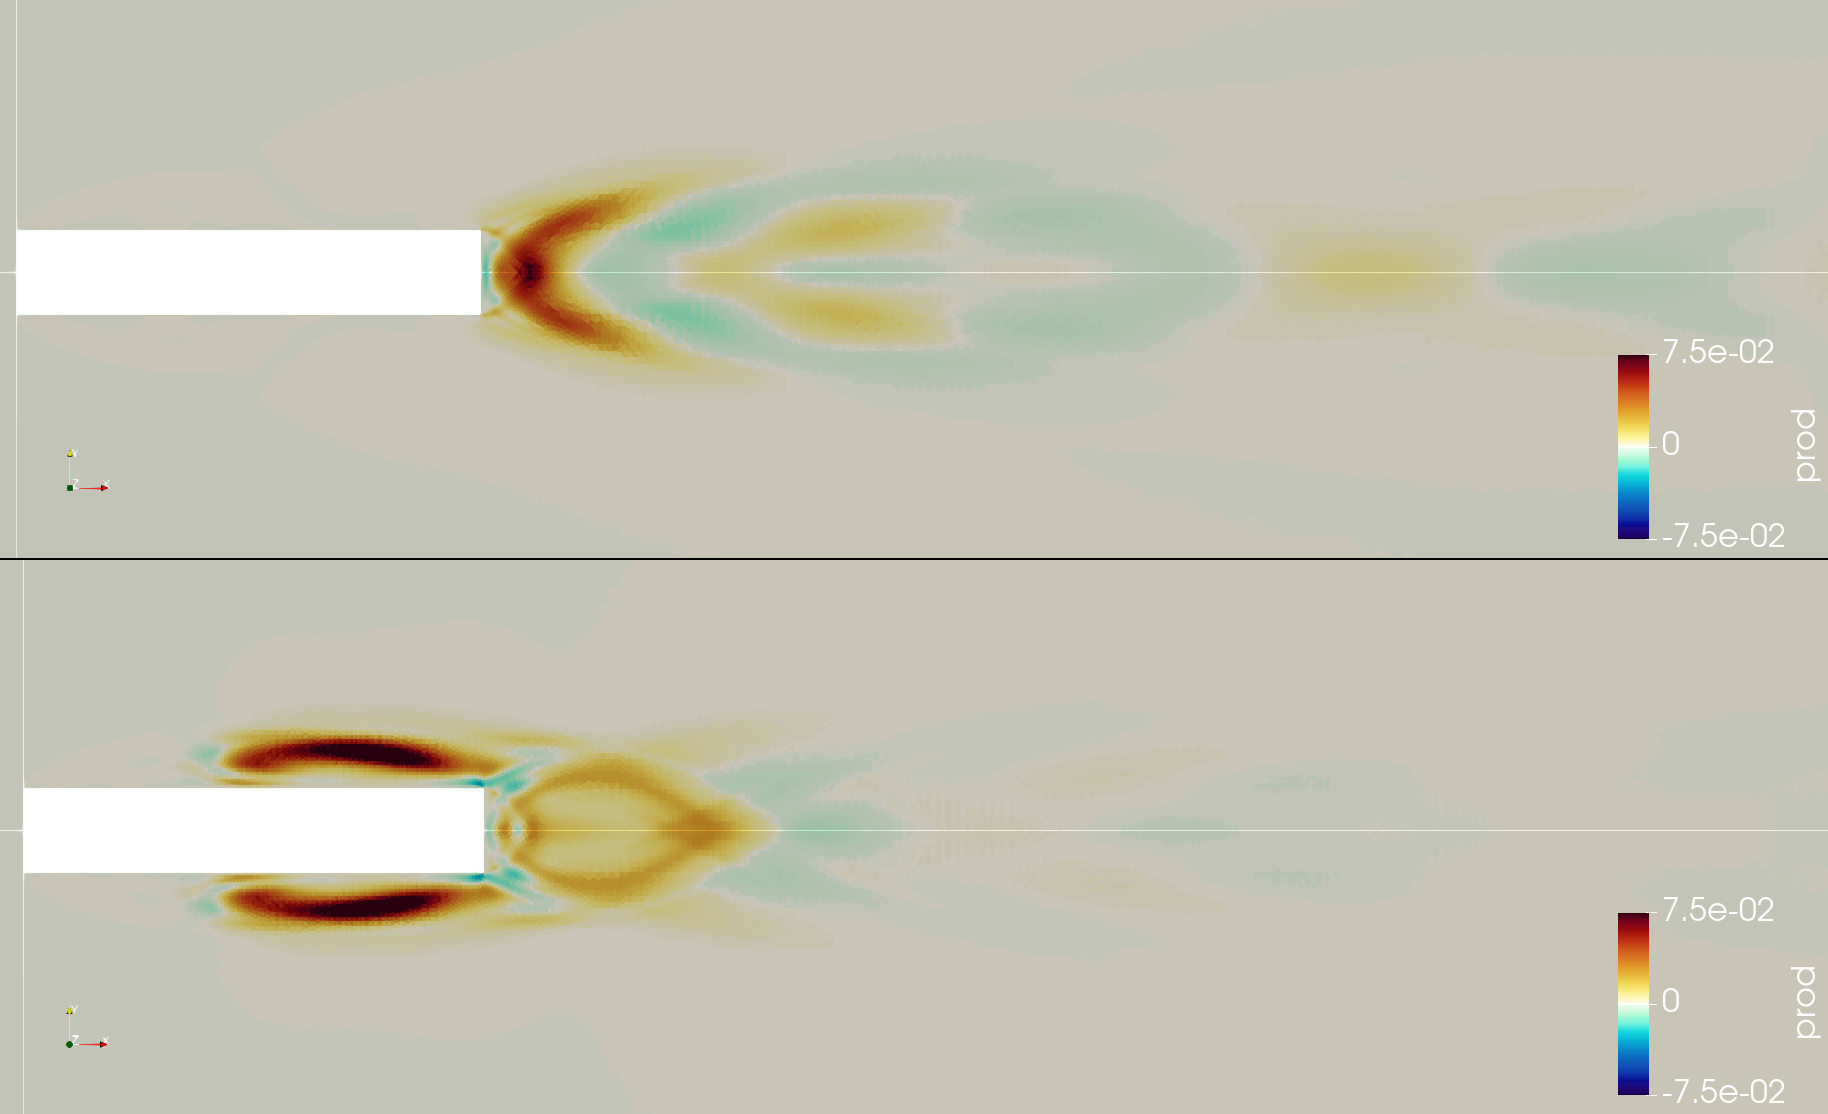
\includegraphics[width=0.49\textwidth]{./fig/AR5p5/Prod_Re450_Re550_beta2.png}
  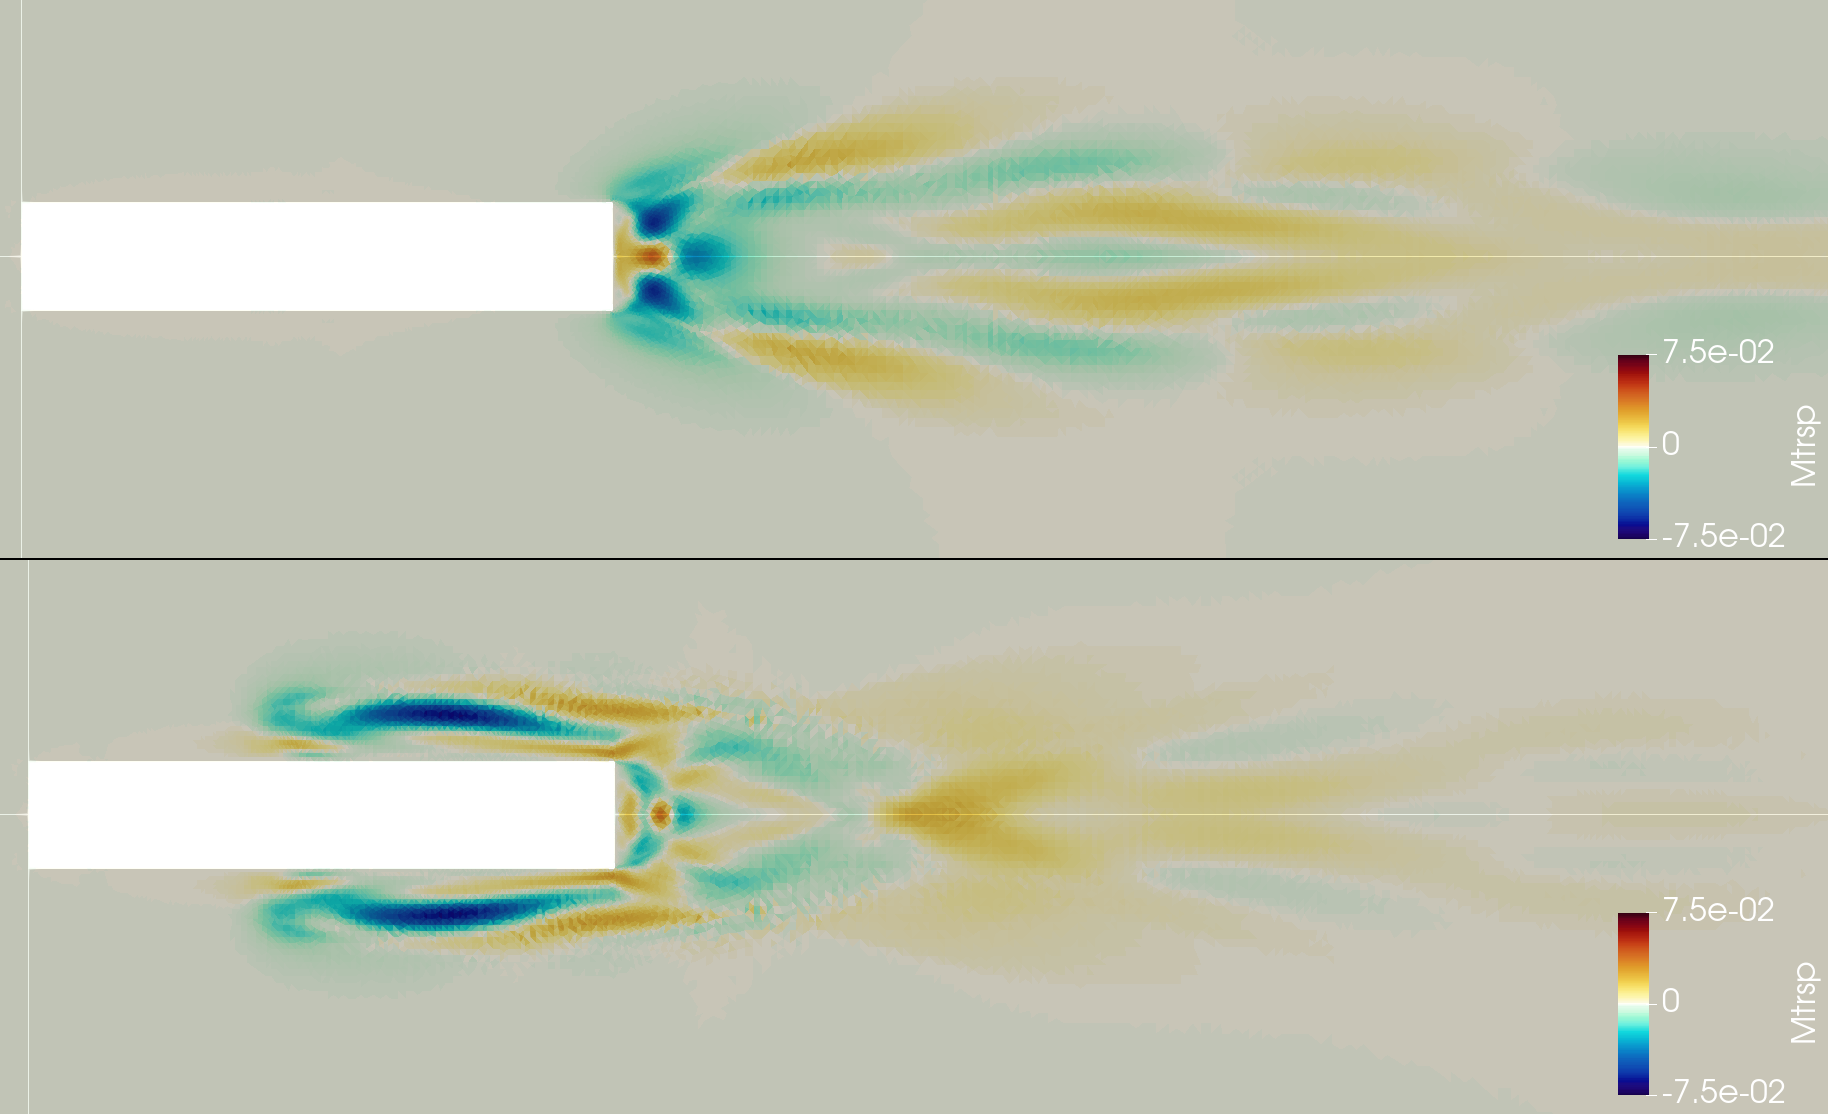
\includegraphics[width=0.49\textwidth]{./fig/AR5p5/Mtrsp_Re450_Re550_beta2.png}
  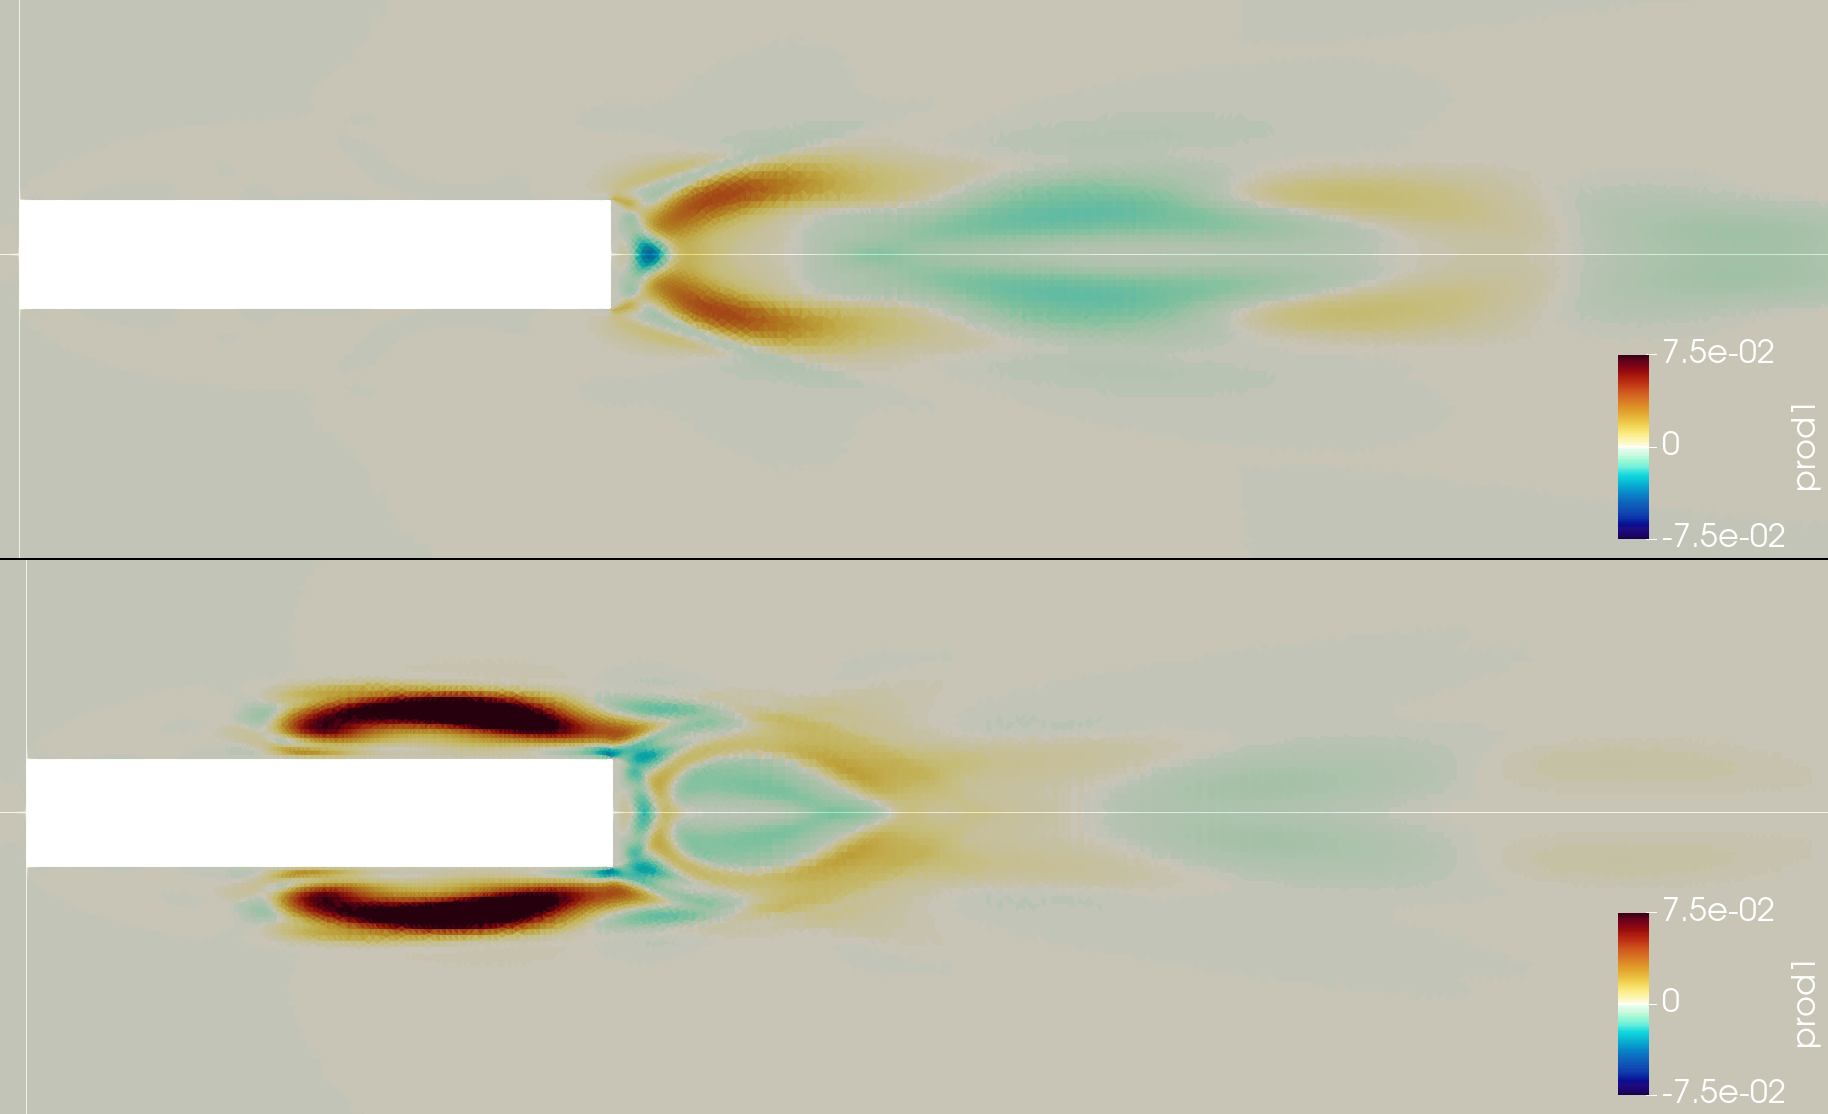
\includegraphics[width=0.49\textwidth]{./fig/AR5p5/Prod1_Re450_Re550_beta2.png}
  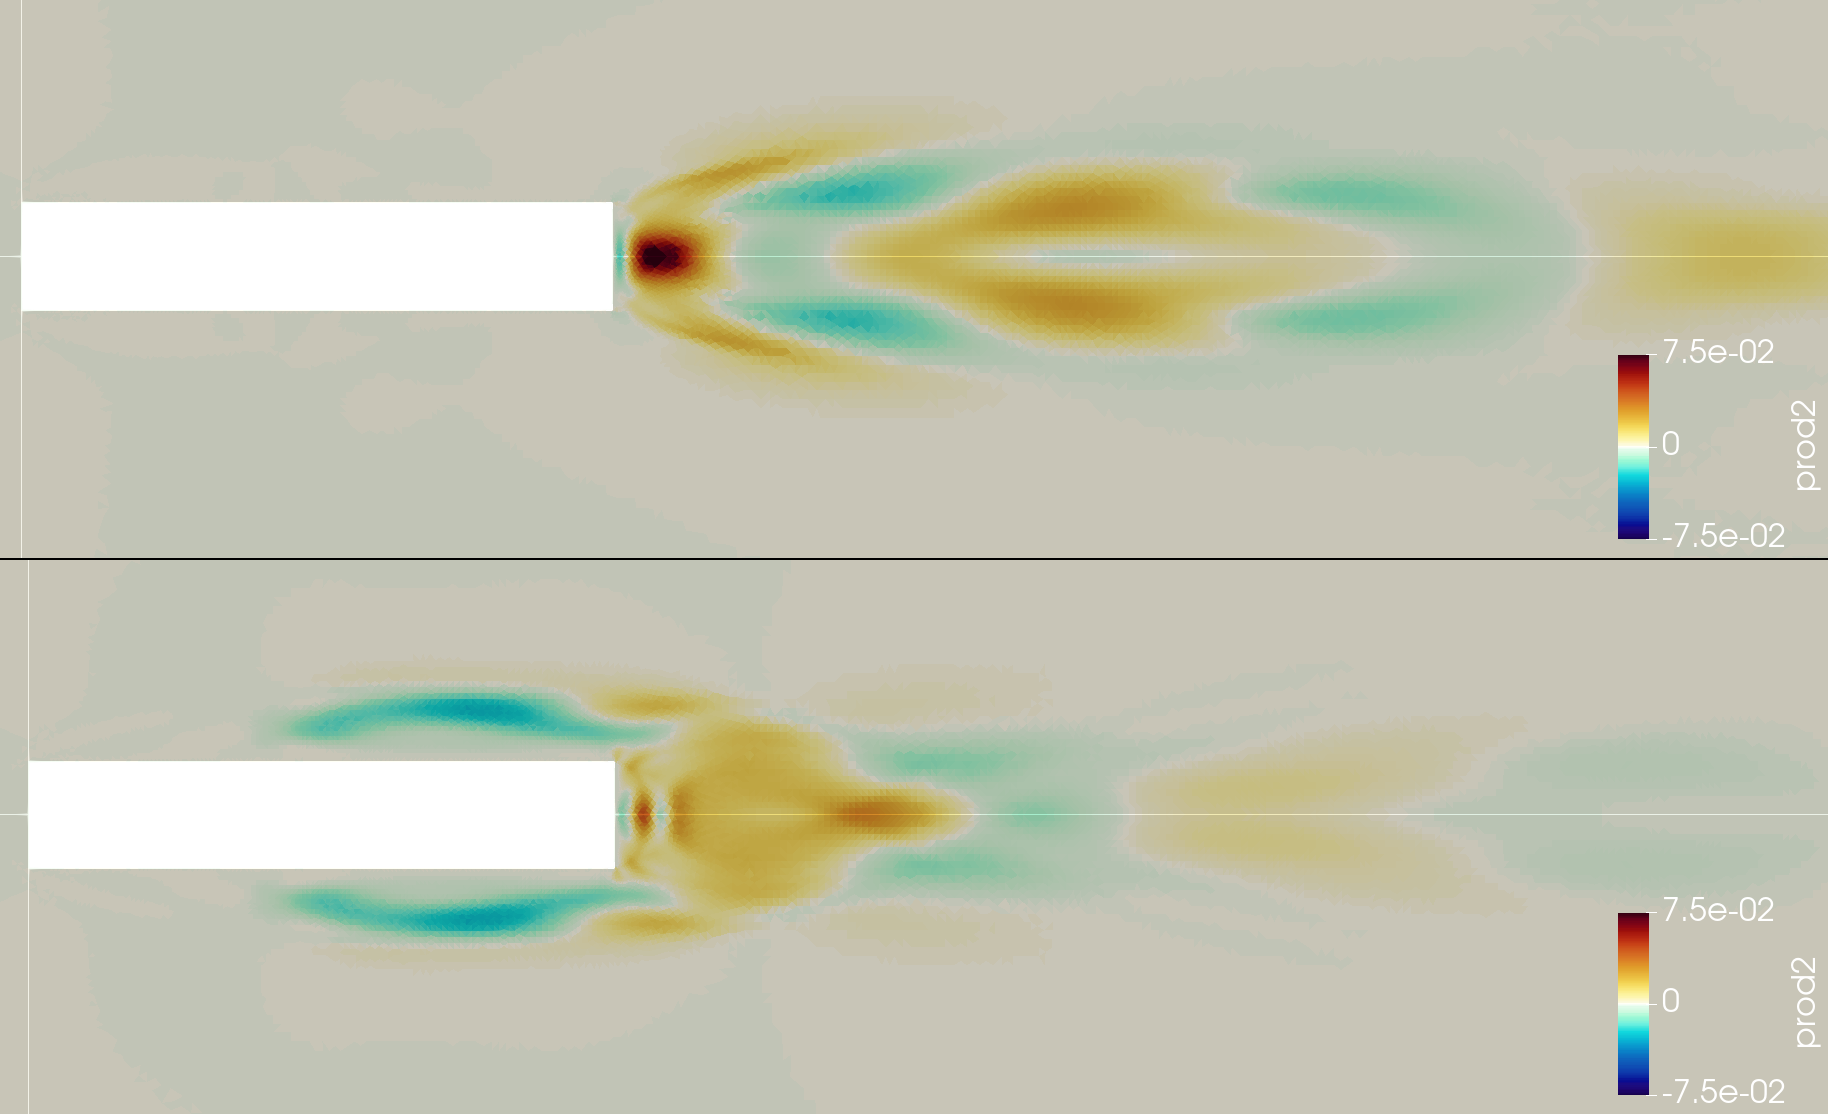
\includegraphics[width=0.49\textwidth]{./fig/AR5p5/Prod2_Re450_Re550_beta2.png}
  \caption{Energy budget for $\AR=5.5$ and mode $A$ (top) and mode $QS$ (bottom). For mode $A$: $Re=450$ and $\beta=2$. For mode $QS$: $Re=550$ and $\beta=2$.}
  \label{fig:ener_budget}
\end{figure}
%
Figure~\ref{fig:ener_budget} presents the energy balance for modes $A$ and $QS$ for an aspect ratio $\AR = 5.5$ and spanwise wavenumber $\beta = 2$. In both cases, the Reynolds number is set close to its critical value, with $Re = 450$ for mode $A$ and $Re = 550$ for mode $QS$, such that the temporal growth rate satisfies $\sigma_r \approx 0$. Under these conditions, the Reynolds–Orr equation simplifies to
\begin{equation*}
 \int_{D} \mathcal{P} \text{d}\Omega = \int_{D} \mathcal{E} \text{d}\Omega \qquad \text{with} \qquad
 \int_{D} \mathcal{A} + \mathcal{T}_p + \mathcal{D} \text{d}\Omega = 0.
\end{equation*} 
%
Our primary focus is on the spatial distributions of the production term $\mathcal{P}$ and the advection term $\mathcal{A}$, in order to identify the regions of the flow where mode amplification is driven by energy production and/or advection.

Consistent with the distinct spatial structures of the two modes, the terms in the energy budget are nonzero in different regions of the domain. For mode $A$, all mechanisms are concentrated downstream of the body, within the wake, whereas for mode $QS$, significant activity is also observed along the lateral sides of the cylinder. For mode $A$, the production term $\mathcal{P}$ is positive along the streamlines that bound the mean recirculating region in the wake—precisely where the base-flow velocity gradients are largest. The alternating regions of $\mathcal{P} > 0$ and $\mathcal{P} < 0$ in the wake reflect the unsteady flapping of the wake, indicating bidirectional energy transfer between the base flow and the perturbation field.
%
In the case of mode $QS$, the most intense production occurs along the lateral surfaces of the body. In this case, $\mathcal{P}$ peaks along the streamlines that define the lateral recirculating regions. However, we also observe positive values of $\mathcal{P}$ in the near wake, indicating that the base flow moves energy to the perturbations in this region as well.

The advection term $\mathcal{A}$ exhibits a contrasting behaviour. It acts as a sink ($\mathcal{A} < 0$), thereby stabilising the flow along the separating shear layers where the base flow velocity $U > 0$: in the near wake for mode $A$, and along the lateral sides of the cylinder for mode $QS$. In contrast, $\mathcal{A}$ becomes a source ($\mathcal{A} > 0$) and contributes to destabilisation within the recirculating regions, where $U < 0$. This is consistent with the interpretation that, within these recirculating zones, the base flow transports perturbations upstream, allowing them to persist and amplify more effectively than in regions where they are simply advected downstream.

To provide further insight, the bottom panels of figure~\ref{fig:ener_budget} show the individual contributions to the production term associated with the streamwise and transverse components of the base flow, $U$ and $V$, respectively; that is, $\mathcal{P}_{uu}$ and $\mathcal{P}_{vv}$.
%
\begin{equation}
  \mathcal{P}_{uu} = - \frac{1}{T} \int_{t_0}^{t_0+T} \left( \hat{u}_j \hat{u}^* + \hat{u}_j^* \hat{u} \right) \frac{\partial U}{\partial x_j} \text{d} t \qquad \text{and} \qquad
\mathcal{P}_{vv} = - \frac{1}{T} \int_{t_0}^{t_0+T} \left( \hat{u}_j \hat{v}^* + \hat{u}_j^* \hat{v} \right) \frac{\partial V}{\partial x_j} \text{d} t.
\end{equation}
%
For both modes, the components of the production term, $\mathcal{P}_{uu}$ and $\mathcal{P}_{vv}$, exhibit distinct spatial distributions. For mode $A$, both components contribute to the overall positive production ($\mathcal{P} > 0$) in the near wake: $\mathcal{P}_{vv}$ dominates near the base of the cylinder, while $\mathcal{P}_{uu}$ is primarily responsible for the production along the separating shear layers. Further downstream in the wake, regions of positive $\mathcal{P}_{uu}$ correlate with negative $\mathcal{P}_{vv}$, and vice versa; this alternating pattern reflects the velocity field induced by the shedding wake vortices.
%
In the case of mode $QS$, the positive $\mathcal{P}$ observed along the lateral sides of the cylinder is entirely due to the $\mathcal{P}_{uu}$ component. In contrast, the positive production region just downstream of the trailing edge arises from $\mathcal{P}_{vv}$.

\iffalse
We close this section by looking at the enstrophy budget. Both modes $A$ and $QS$, indeed, are responsible for the flow three-dimensionalisation and, threfore, they are resposible for the generation of (streamwise) vorticity in the flow. As for the energy, we start from the governing equation for the perturbation and derive the budget for the enstrophy defied as $\hat{\omega}_i \hat{\omega}_i^*$. Specifically, the enstrophy equation is obtained starting from the equation governing the vorticity pertubation $\hat{\omega}_i$ multiplied by $\hat{\omega}_i^*$ and summing the result to the conjugate of the same equation multiplied for $\hat{\omega}_i$. The results is:
%
\begin{equation}
  \begin{gathered}
  \frac{2 \Re{\sigma}}{T} \int_{t_0}^{t_0+T} \hat{\omega}_i \hat{\omega}_i^* \text{d}t =  
  \underbrace{
  - \frac{1}{T} \int_{t_0}^{t_0+T} \left( \hat{\omega}_i^* \hat{u}_j + \hat{\omega}_i u_j^* \right) \frac{\partial \Omega_i}{\partial x_j} \text{d}t
  + \frac{1}{T} \int_{t_0}^{t_0+T}    i \beta \Omega_3 \left( \hat{u}_i \hat{\omega}_{i}^* - \hat{u}_i^* \hat{\omega}_i \right)  \text{d} t}_{\mathcal{P}^\omega} \\
  \underbrace{  - \frac{1}{T} \int_{t_0}^{t_0+T} U_j \frac{\partial \hat{\omega}_i \hat{\omega}_i^* }{\partial x_j} \text{d} t }_{\mathcal{A}^\omega}
  \underbrace{
  + \frac{1}{T} \int_{t_0}^{t_0+T} \left( \hat{\omega}_i^* \hat{\omega}_j + \hat{\omega}_i \hat{\omega}_j^* \right) \frac{\partial U_i}{\partial x_j} \text{d} t }_{\mathcal{V}^\omega} + \\
  + 
  \underbrace{\frac{1}{T} \int_{t_0}^{t_0+T}    \frac{1}{Re} \frac{\partial}{\partial x_j} \left( \frac{\partial \hat{\omega}_i \hat{\omega}_i^*}{\partial x_j} \right) \text{d} t }_{\mathcal{D}^{\omega}} -
 \underbrace{ \frac{1}{T} \int_{t_0}^{t_0+T} \frac{1}{Re} \left( 2 \frac{\partial \hat{\omega}_i}{\partial x_j} \frac{\partial \hat{\omega}_i^*}{\partial x_j} + 2 \beta^2 \hat{\omega}_i \hat{\omega}_i^* \right) \text{d} t }_{\mathcal{E}^\omega}.
  \end{gathered}
\end{equation}
%
Like the energy equations the terms of this equations describe the physical mechanism that are responsible for the exponential growth of the enstrophy in the linear regime for $Re \approx Re_c$. At the right-hand side, we recognise the production $\mathcal{P}^\omega$, advection $\mathcal{A}^\omega$, viscous diffusion $\mathcal{D}^\omega$ and dissipation $\mathcal{E}^\omega$ terms. Here the pressure transport is not present due to the action of the the curl operator to obtain the equaiton for $\hat{\omega}_i$. The additional $\mathcal{V}$ term comes from the vortex stretching term, which differentiates enstrophy from energy. It describes the production of enstrophy due to the interaction of vorticity $\omega_i$ and the stretching vecotr $\omega_i \partial U_i/\partial x_j$.

\begin{figure}
  \centering
  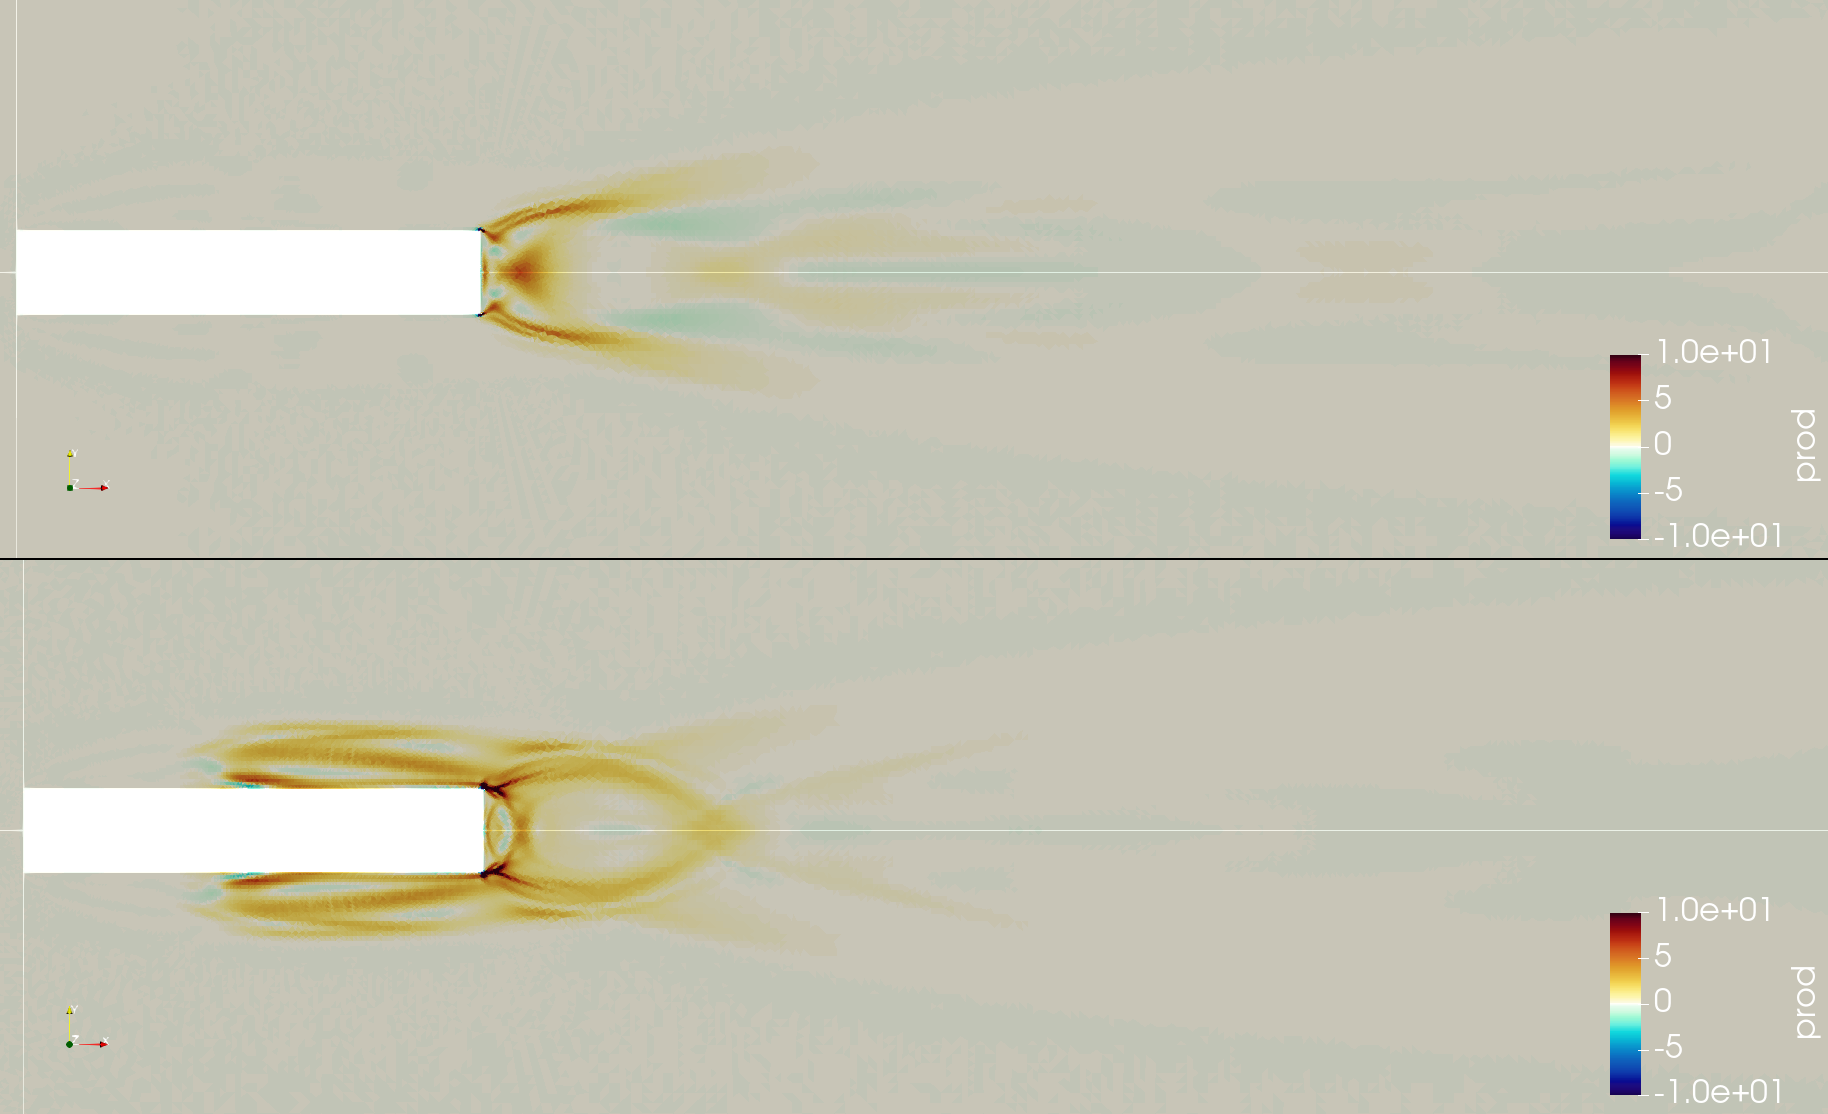
\includegraphics[width=0.49\textwidth]{./fig/AR5p5/Prod_Re450_Re550_beta2_enst.png}
  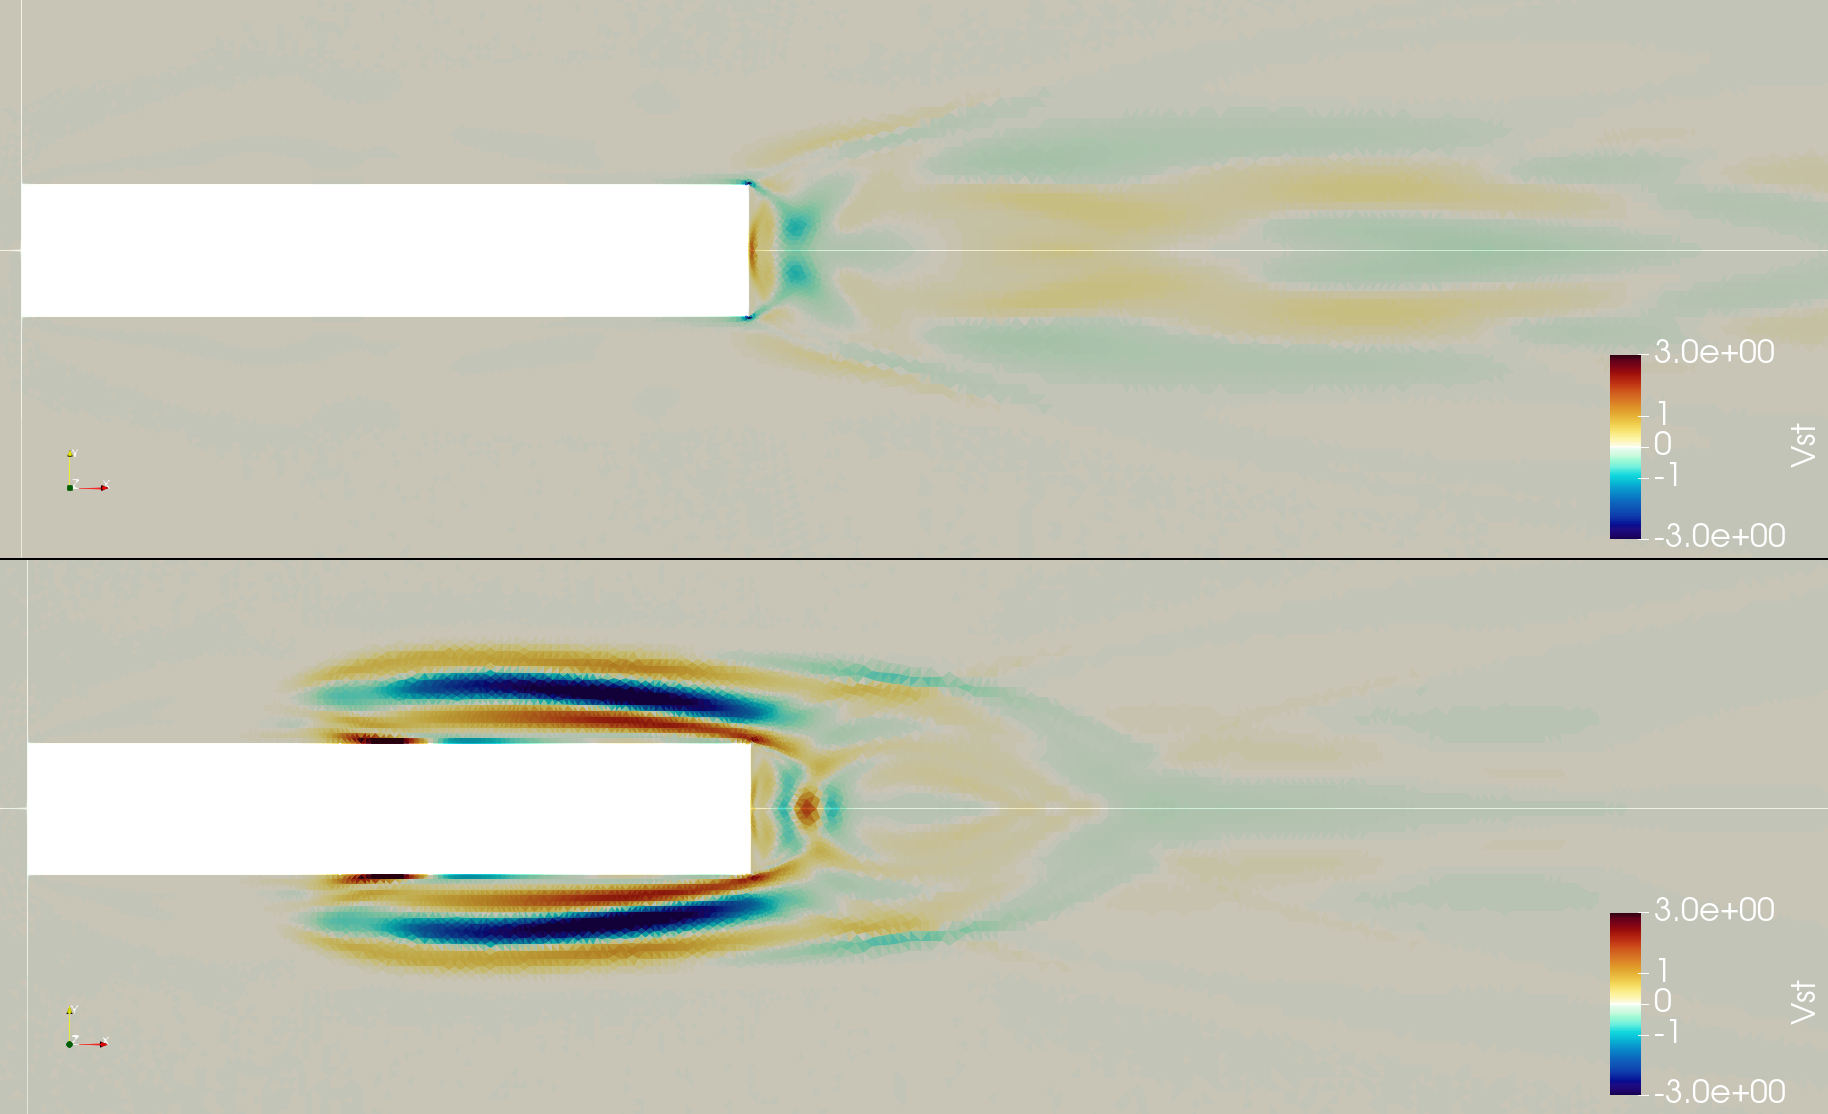
\includegraphics[width=0.49\textwidth]{./fig/AR5p5/Vst_Re450_Re550_beta2_enst.png}
  \caption{Enstrophy budget for $\AR=5.5$ and mode $A$ (top) and mode $QS$ (bottom). For mode $A$: $Re=450$ and $\beta=2$. For mode $QS$: $Re=550$ and $\beta=2$.}
  \label{fig:enst_budget}
\end{figure}

Figure \ref{fig:enst_budget} shows separately $\mathcal{P}^\omega$ and $\mathcal{V}^\omega$ for the two modes. We observe that $\mathcal{P}^\omega$ is mostly positive for both modes, being maximum along the shear layers delimiting the average recirculating regions where the base-flow velocity gradients are maxima. The vortex stretching $\mathcal{V}$ term, instead, acts as a sink or a source depending on the flow region.
\fi

\subsection{The competing $A$ and $QS$ modes}

\textcolor{red}{XX Add non linear simulations for $\AR=5.5$ for $Re=450,475,500,525,550$ con spettri, visualizzazioni. Se serve proviamo a vedere anche i POD modes}


\subsection{Non linear simulations}

\begin{figure}
  \centering
  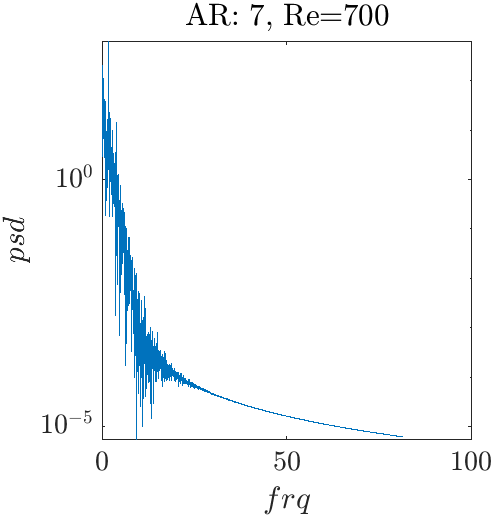
\includegraphics[width=0.24\textwidth]{./fig/nnl/psdAR7RE700.png}
  %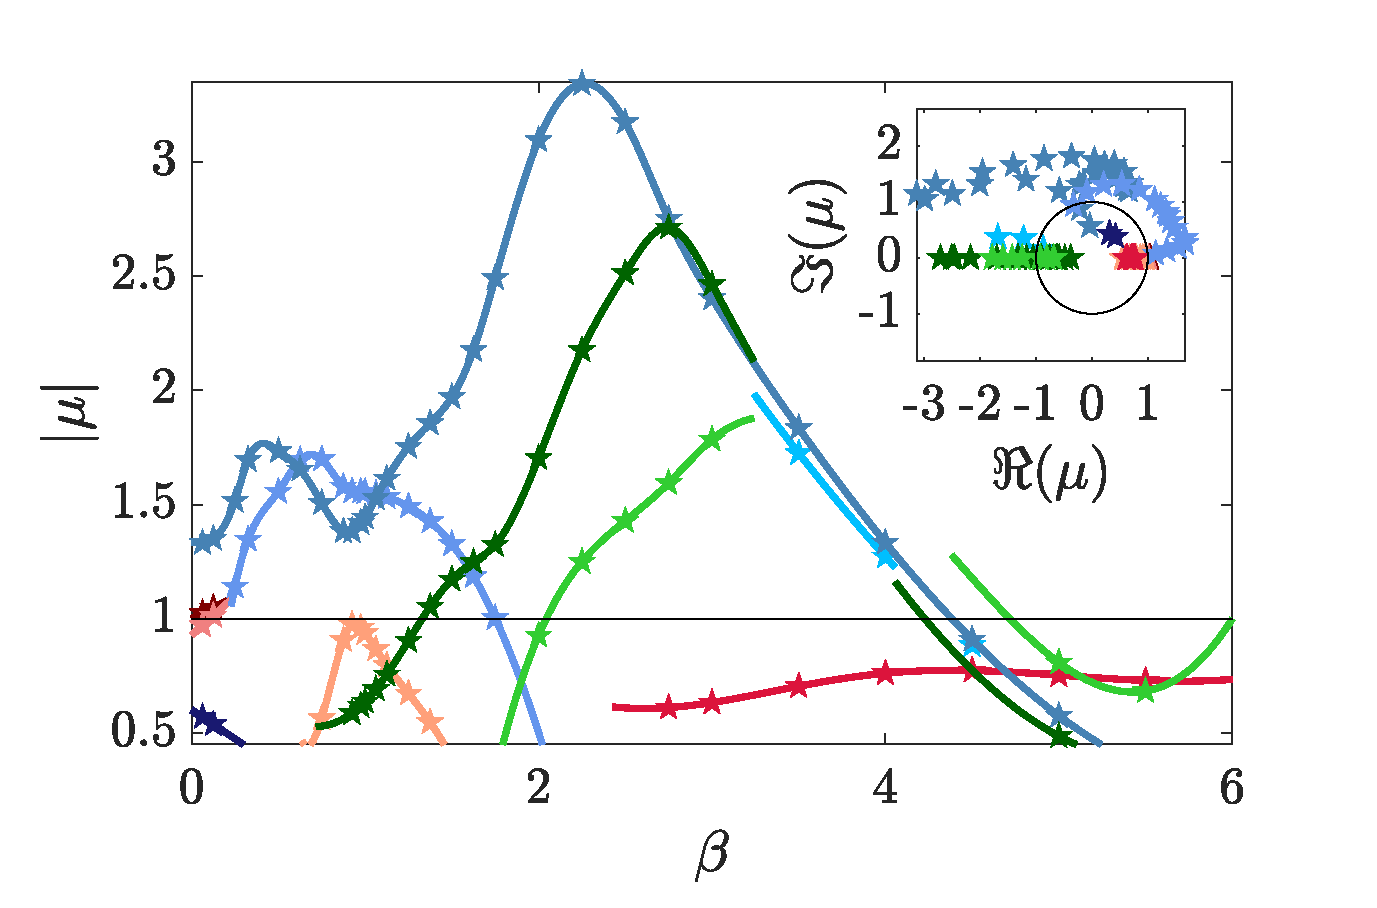
\includegraphics[width=0.49\textwidth]{./fig/AR1p25/mu_beta_Re250.eps}
  \caption{Psd for $\AR=4.5$ at different $Re$.}
  \label{fig:ClCd}
\end{figure}


\begin{figure}
  \centering
  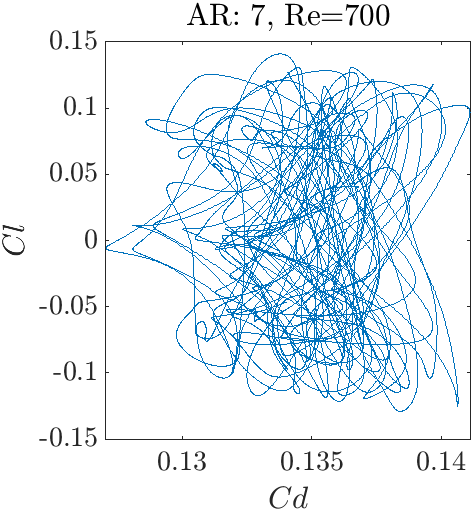
\includegraphics[width=0.24\textwidth]{./fig/nnl/ClCdAR7RE700.png}
  %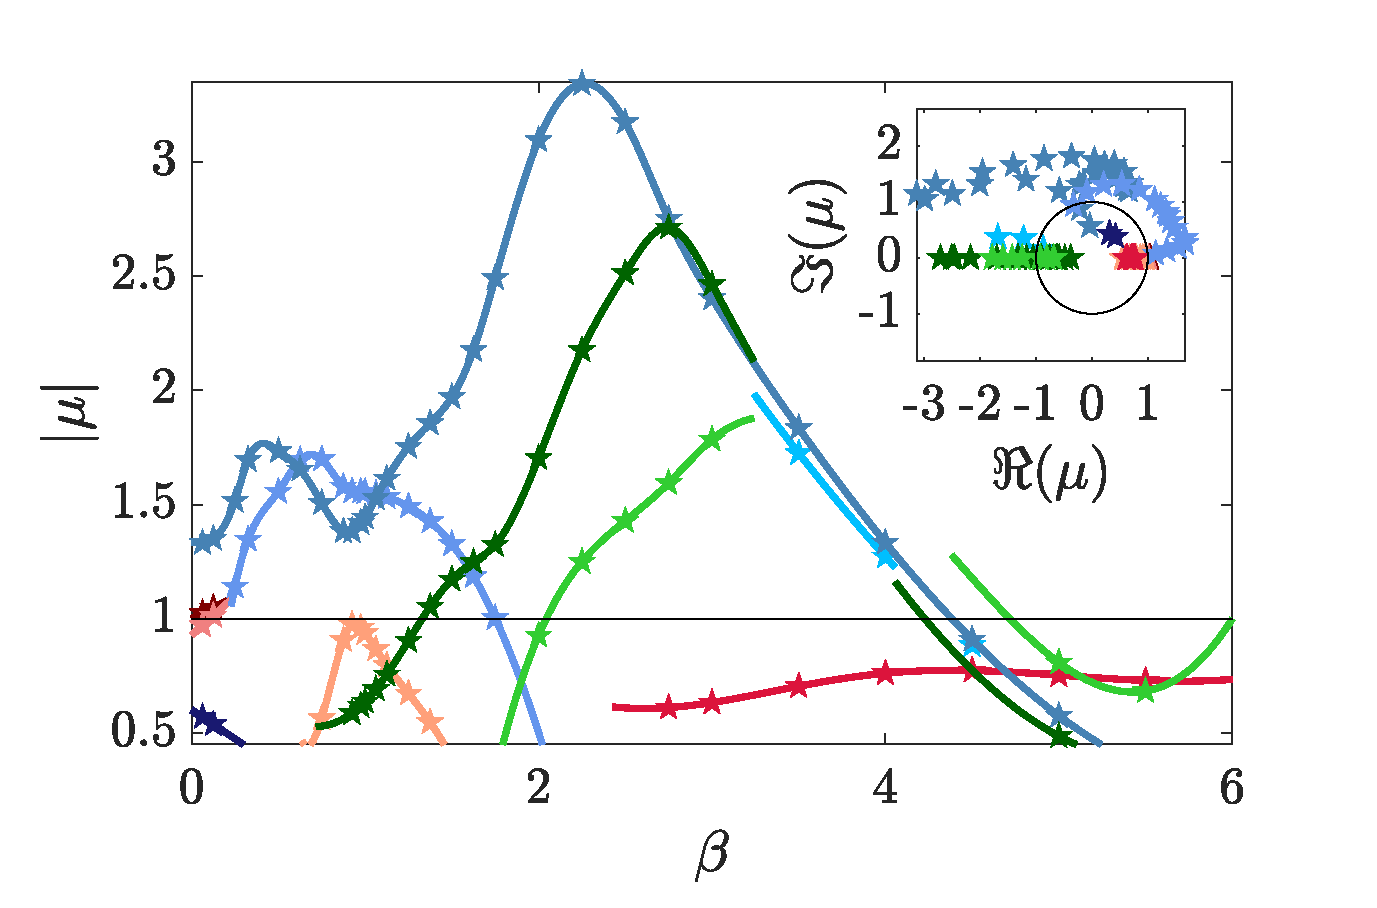
\includegraphics[width=0.49\textwidth]{./fig/AR1p25/mu_beta_Re250.eps}
  \caption{Cl vs Cd for $\AR=5.5$ at different $Re$.}
  \label{fig:ClCd}
\end{figure}


\begin{figure}
  \centering
  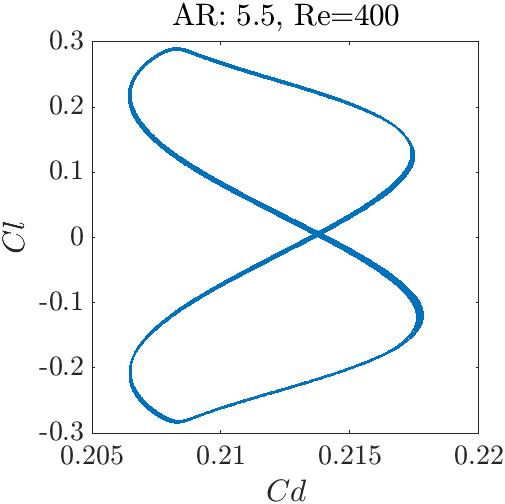
\includegraphics[width=0.24\textwidth]{./fig/nnl/ClCdAR5.5RE400.png}
  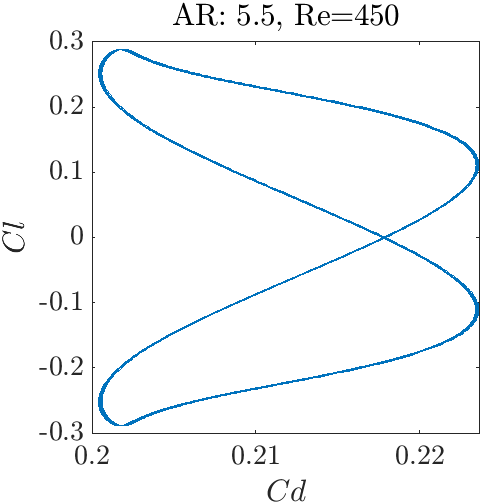
\includegraphics[width=0.24\textwidth]{./fig/nnl/ClCdAR5.5RE450.png}
  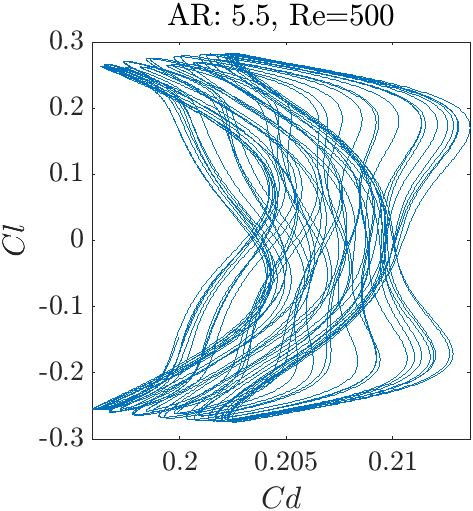
\includegraphics[width=0.24\textwidth]{./fig/nnl/ClCdAR5.5RE500.png}
  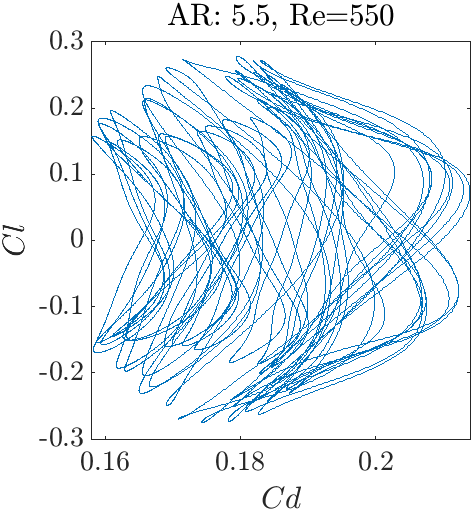
\includegraphics[width=0.24\textwidth]{./fig/nnl/ClCdAR5.5RE550.png}
  %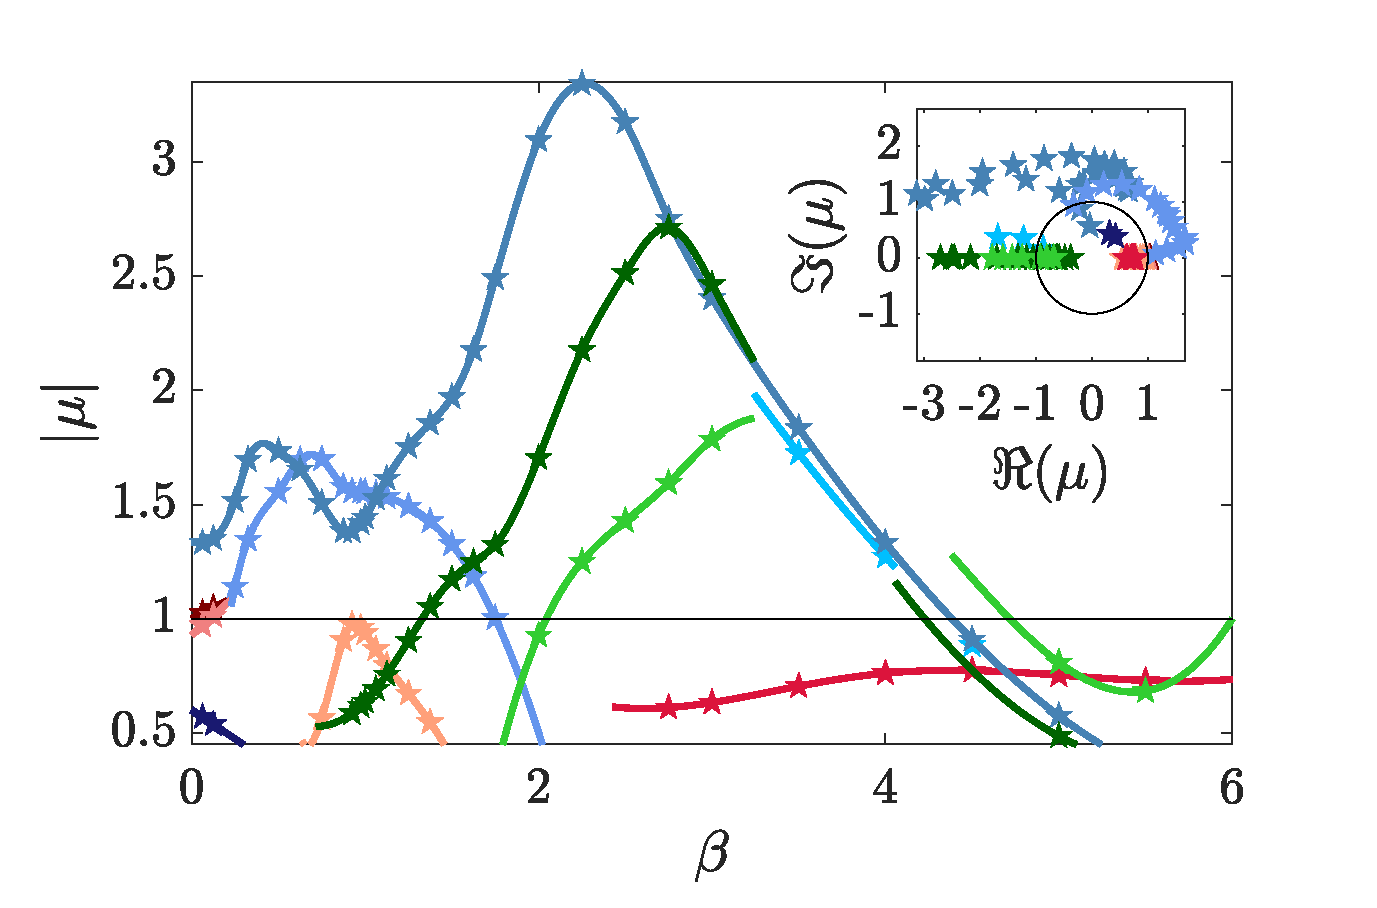
\includegraphics[width=0.49\textwidth]{./fig/AR1p25/mu_beta_Re250.eps}
  \caption{Cl vs Cd for $\AR=5.5$ at different $Re$.}
  \label{fig:ClCd}
\end{figure}

\begin{figure}
  \centering
  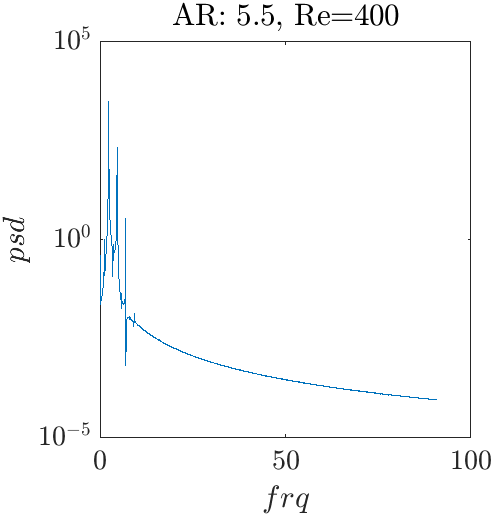
\includegraphics[width=0.24\textwidth]{./fig/nnl/psdAR5.5RE400.png}
  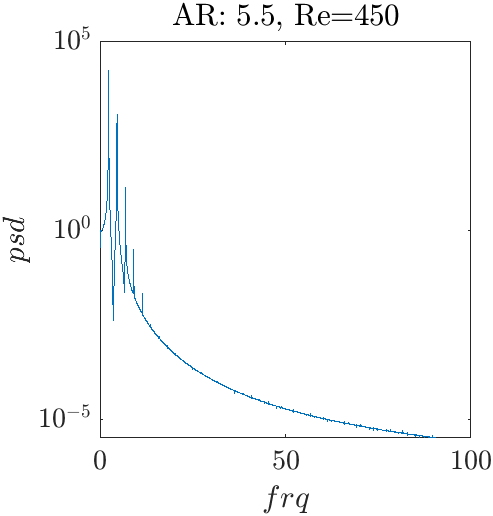
\includegraphics[width=0.24\textwidth]{./fig/nnl/psdAR5.5RE450.png}
  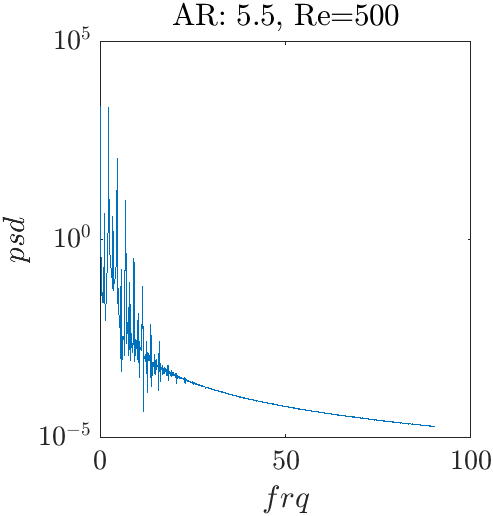
\includegraphics[width=0.24\textwidth]{./fig/nnl/psdAR5.5RE500.png}
  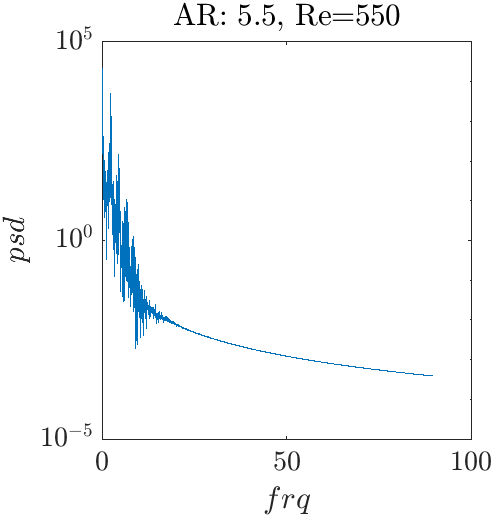
\includegraphics[width=0.24\textwidth]{./fig/nnl/psdAR5.5RE550.png}
  %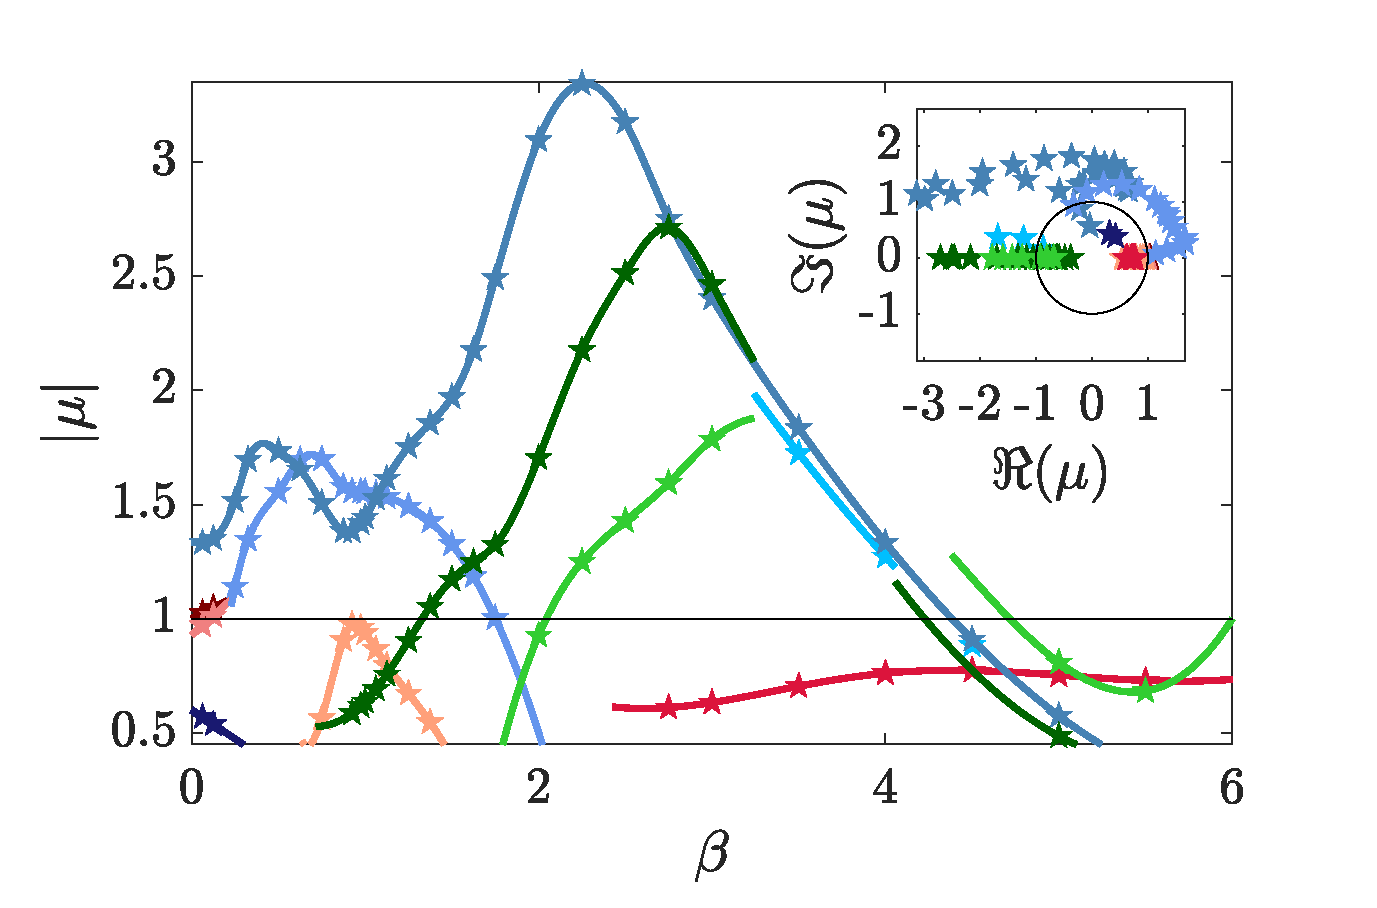
\includegraphics[width=0.49\textwidth]{./fig/AR1p25/mu_beta_Re250.eps}
  \caption{Psd for $\AR=5.5$ at different $Re$.}
  \label{fig:ClCd}
\end{figure}

\iffalse
XX FIN QUI XX

Figure \ref{} shows the unstable branches of Floquet multipliers for $5.25 \le \AR \le 5.75$ ($n=2$ oblique brach), $\AR=6,7$ ($n=2$ horizontal branch) and $\AR=9$ ($n=3$ oblique branch). The scanario changes with $\AR$ with different modes becoming unstable, in agreement with the change of the base flow dynamics. The case with $\AR=5$ has been discussed in \cite{chiarini-quadrio-auteri-2022d}.

We start characterising the $n=2$ and $n=3$ oblique branches, i.e. $5.25 \le \AR \le 5.75$ and $\AR=9$. For these $\AR$s we find three different modes, with the order with which they become unstable that changes with the aspect ratio. For $5 \le \AR \le 5.25$ and $\AR=9$ the first mode to become unstable is mode $QS$. This mode is characterised by a pair of complex conjugate Floquet multipliers having negative real part and almost null imaginary part, with $\mu = (xx,xx)$ for $\AR=5.5$, $Re=450$ and $\beta=2$. \textcolor{red}{XX Add figure with the real and complex partx XX} This instability is driven by the inviscid interaction of the LE vortices that are simultaneously accomodated along the lateral sides of the cylinder \citep{pierrhumbert-widnall-1982}, and is characterised by a characteristic spanwise wavenumber of $\beta \approx 2$, which corresponds to a wavelength of $\lambda \approx \pi$


XX PER $\AR=5.5$ per $Re \in (450,400)$ sembra che ci sia di nuovo effetto della scia secondaria. E' presente a Re bassi e poi sparisce a Re piu alti. Bisogna caratterizzare questo aspetto in generale. Quindi per evitare problemi, per Re intermedi rifaccio Floquet per una dimensionel del dominio più piccola che mi garantisce la periodicità XX

\begin{itemize}
  \item Here we look at the second oblique branch of the $St_L-\AR$ plane. Here we have already found that for $\AR=5$ the first mode to become unstable is mode QS, i.e. the quasi-subharmonic mode.
  \item We now investigate what happens when increasing $\AR$. We recall that this is the range where the vortex shedding is dominated by the TE. This means that the dynamics of the TE vortex shedding dominates and is not directly influenced by the vortex shedding from the LE as in the oblique branches. As shown in figure \ref{fig:mult_AR5s}, for $\AR=5$ the only unstable mode is of subharmonic nature and is the so-called mode $QS$. As $\AR$ is increased, instead, a new mode of synchronous nature appears (in this case the multipliers are real and positive). For $\AR=5.25$ this mode is stable. For $\AR=5.35$ this mode approaches the unit circle. For $\AR=5.5$ this mode is unstable, and its growth rate is larger than the corresponding one associated with mode $QS$. The second mode here detected resembles mode $A$ for the wake past short cylinders. 
  \item Mode QS is an unstable mode of the recirculating region along the lateral sides of the cylinder. This is visualised in figure \ref{fig:mult_AR5s} (note that the mote is maximum there and not in the wake). For additional details see \citep{chiarini-etal-2022}. The synchronous mode, instead, is an unsteady mode of the wake and share several properties with the classical mode $A$ of the circular cylinder.
  \item For the arise of the new mode $A$ in the $5.25 \le \AR \le 5.75$ regime look at the works by Aleksyuk \& Heil (2023) and Aleksyuk \& Heil (2024). To answer the question "Why this mode is not detected for $\AR=5$? Why it becomes unstable only at larger $\AR$?" We can start looking whether also in this case the mechanism proposed by Aleksyuk \& Heil (2023,2024) works. If this is the case, we can see if for $\AR=5$ we actually have something different. 
  \item \textcolor{blue}{For $\AR=5.5$ we have that mode $A'$ and $QS$ become unstable is short succession. We can use DNS to see how do they appear. We start from $Re=450$ and then increase progressively $Re$. Look for an indicator to characterise how the flow moves from one regime to the other.}
\end{itemize}

\begin{figure}
  \centering
  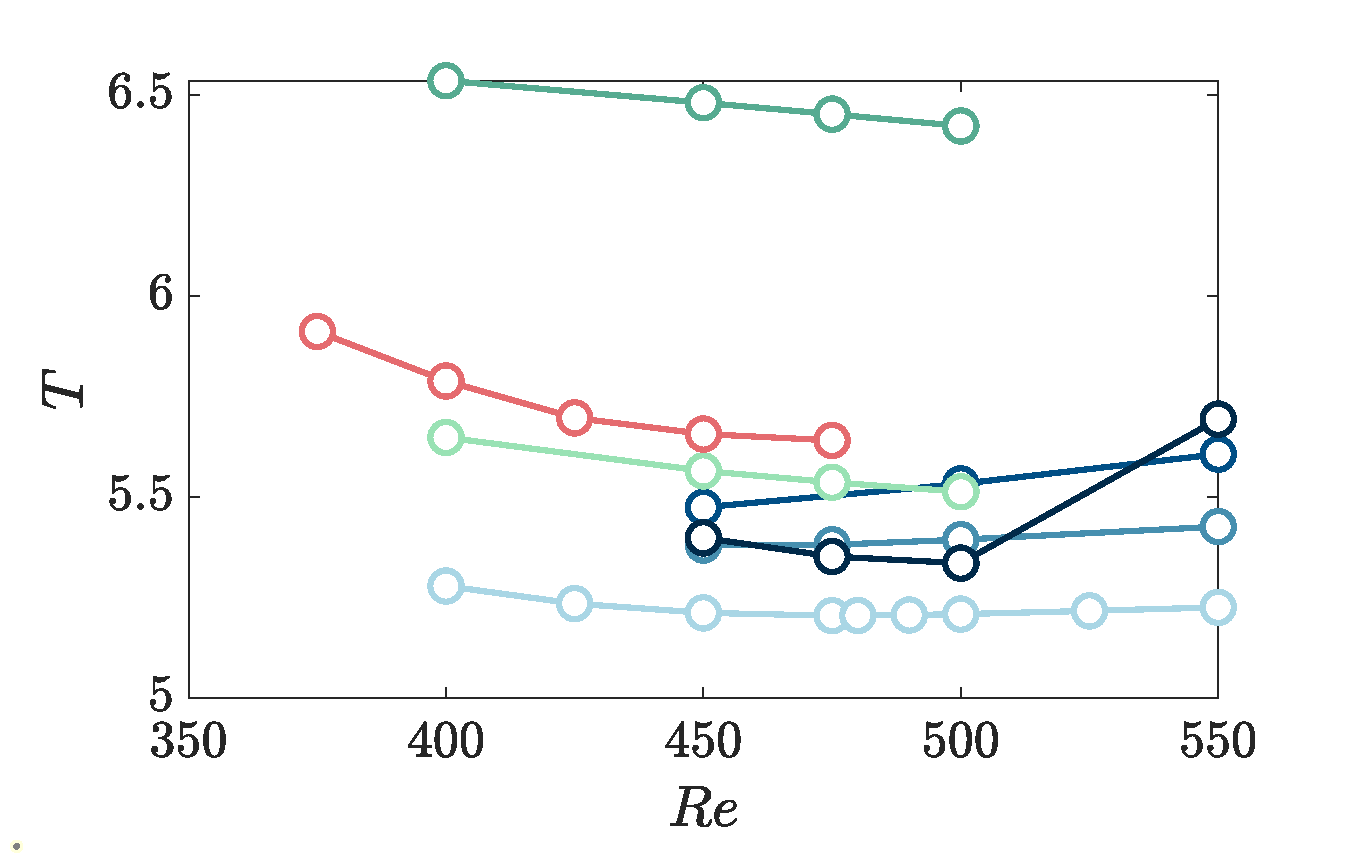
\includegraphics[width=0.49\textwidth]{./fig/long/T_Re.eps}
  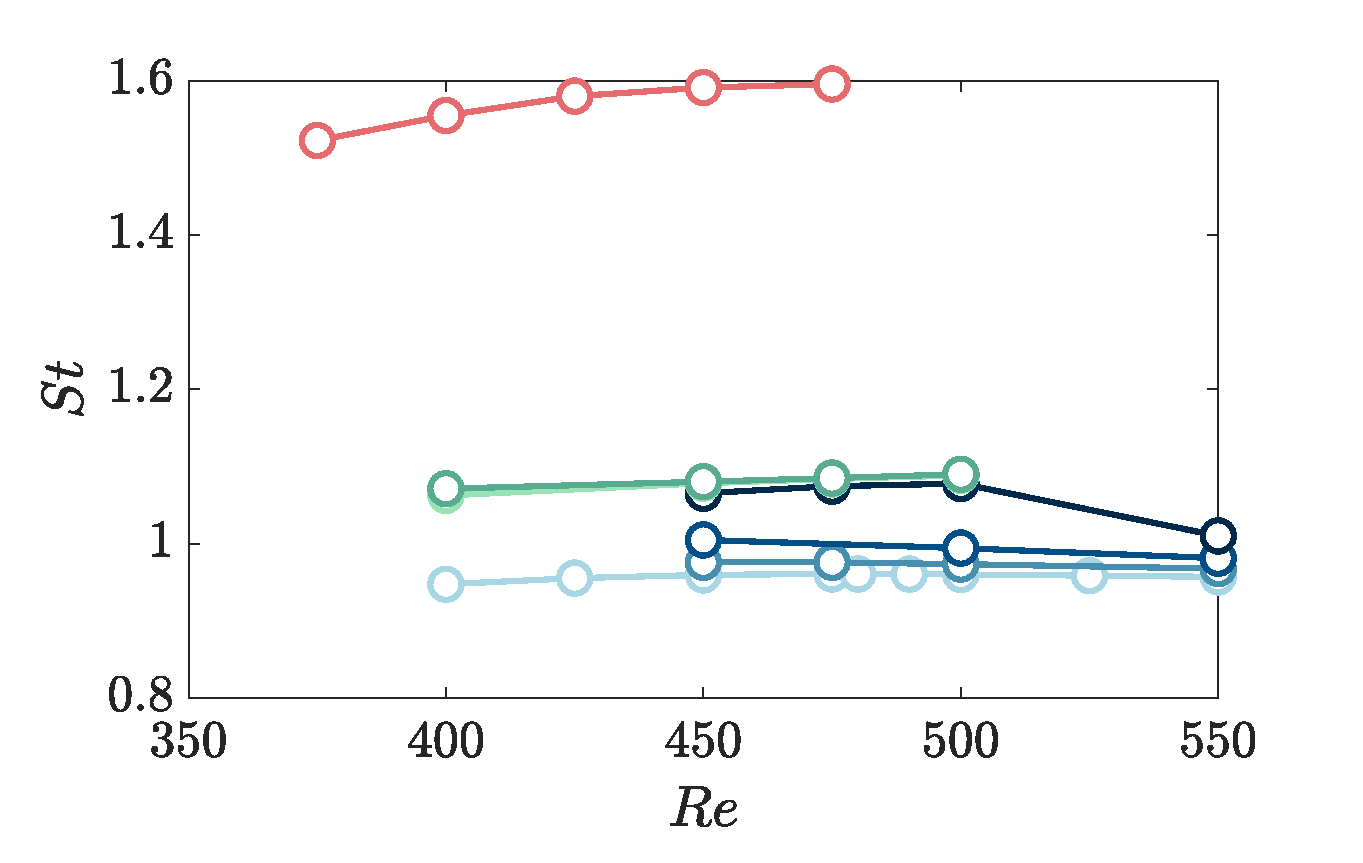
\includegraphics[width=0.49\textwidth]{./fig/long/St_Re.eps}
  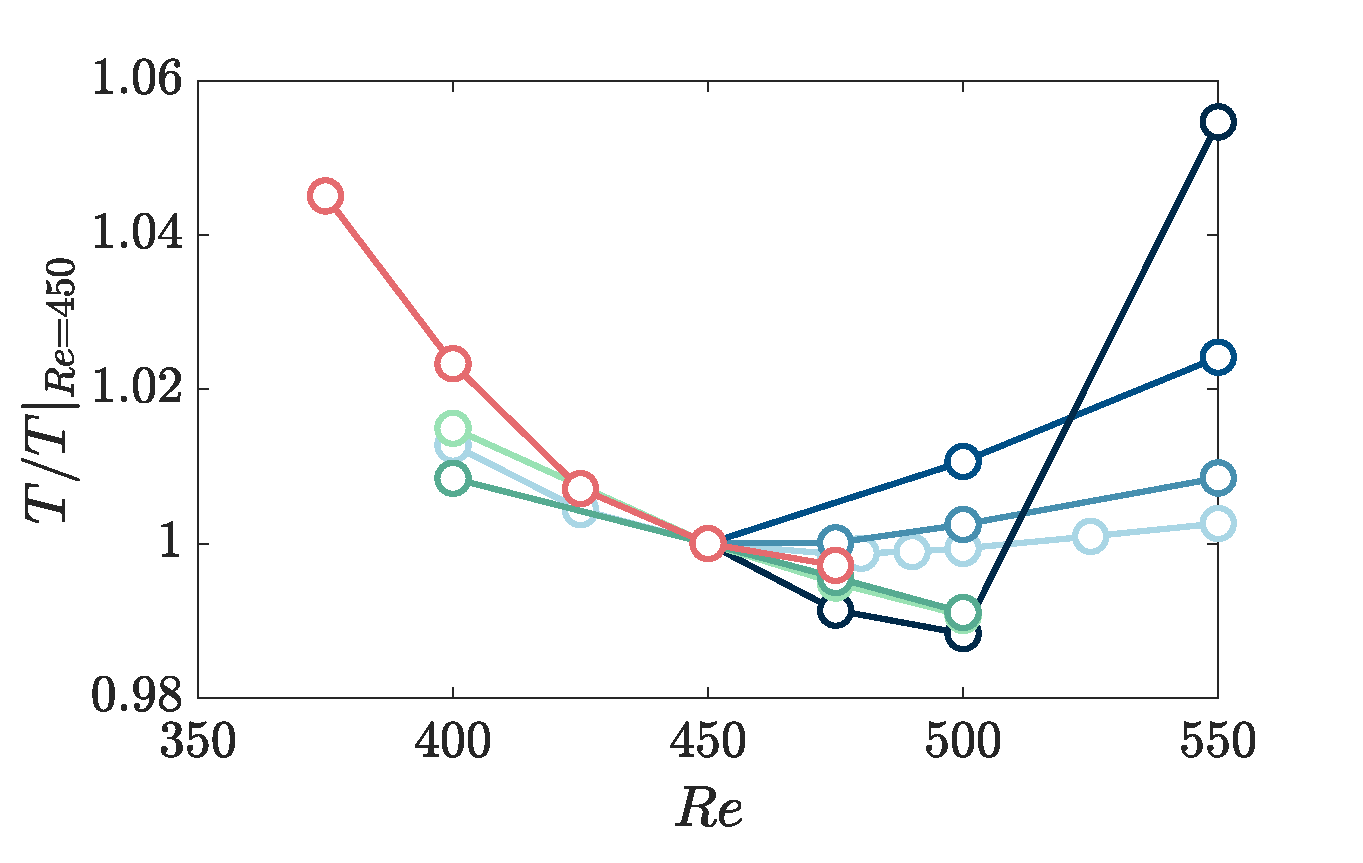
\includegraphics[width=0.49\textwidth]{./fig/long/T_Re_b.eps}
  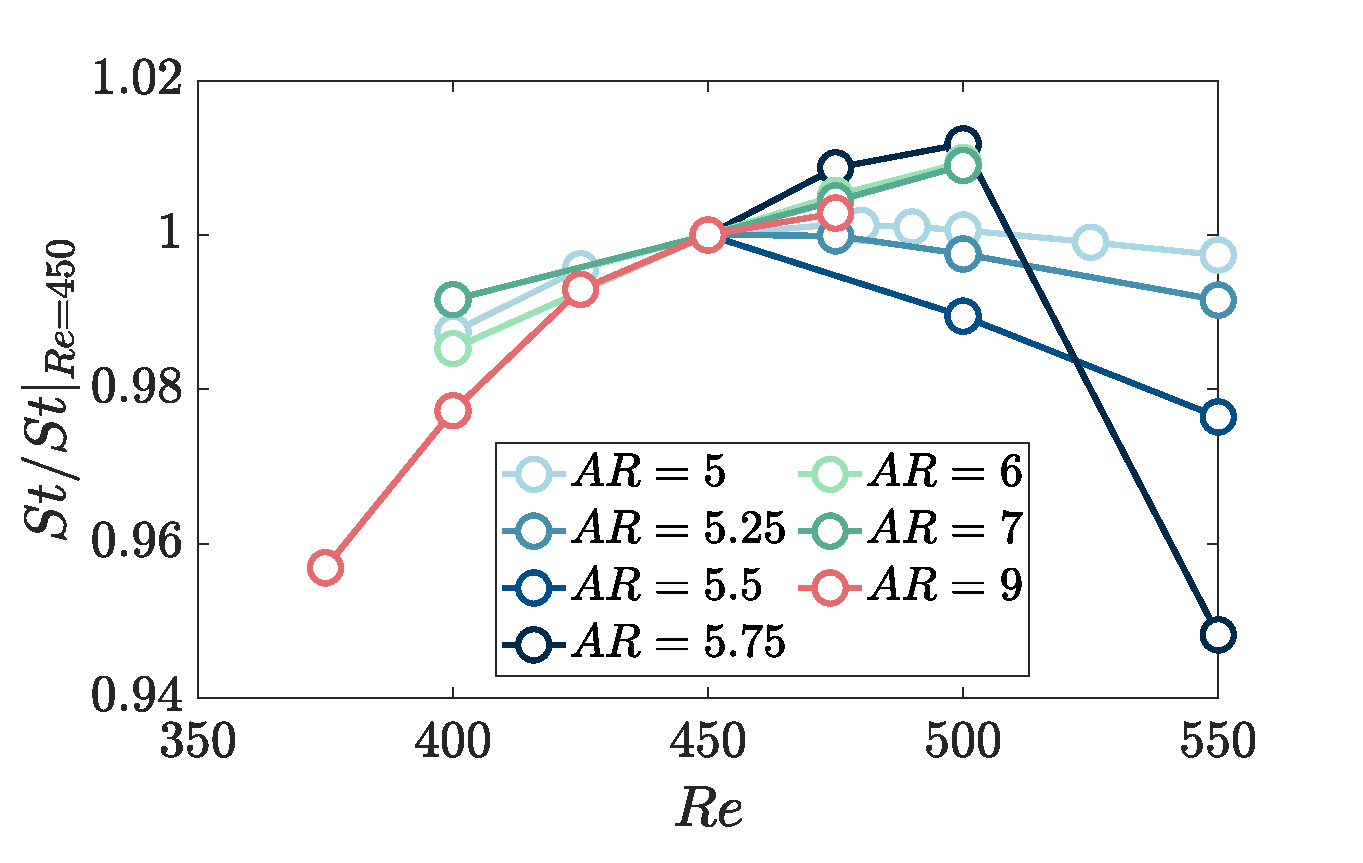
\includegraphics[width=0.49\textwidth]{./fig/long/St_Re_b.eps}
  \caption{xx}
  \label{fig:T_St_Re_long}
\end{figure}


\begin{figure}
  \centering
  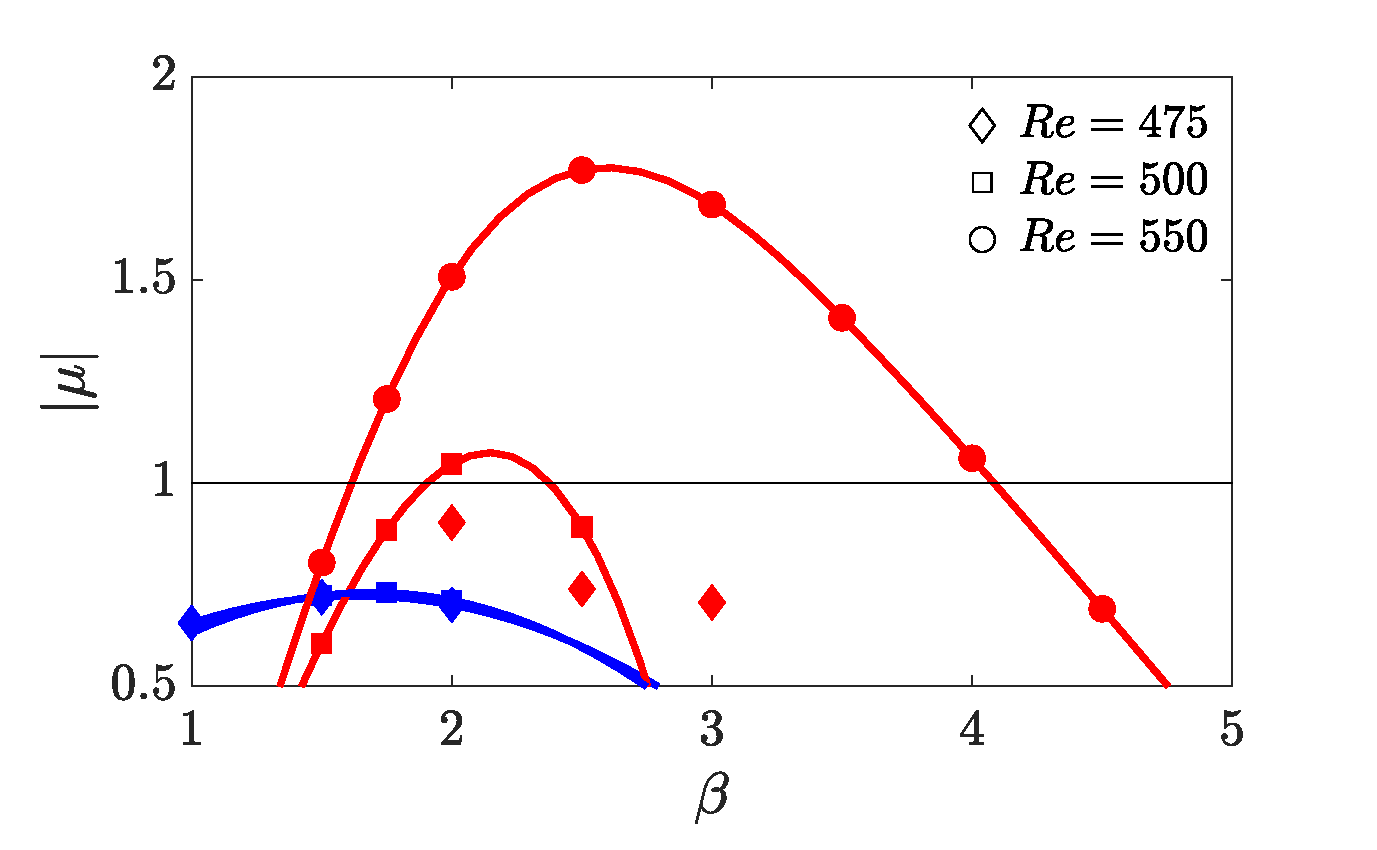
\includegraphics[width=0.49\textwidth]{./fig/AR5s/multipliers_AR5p25.eps}  
  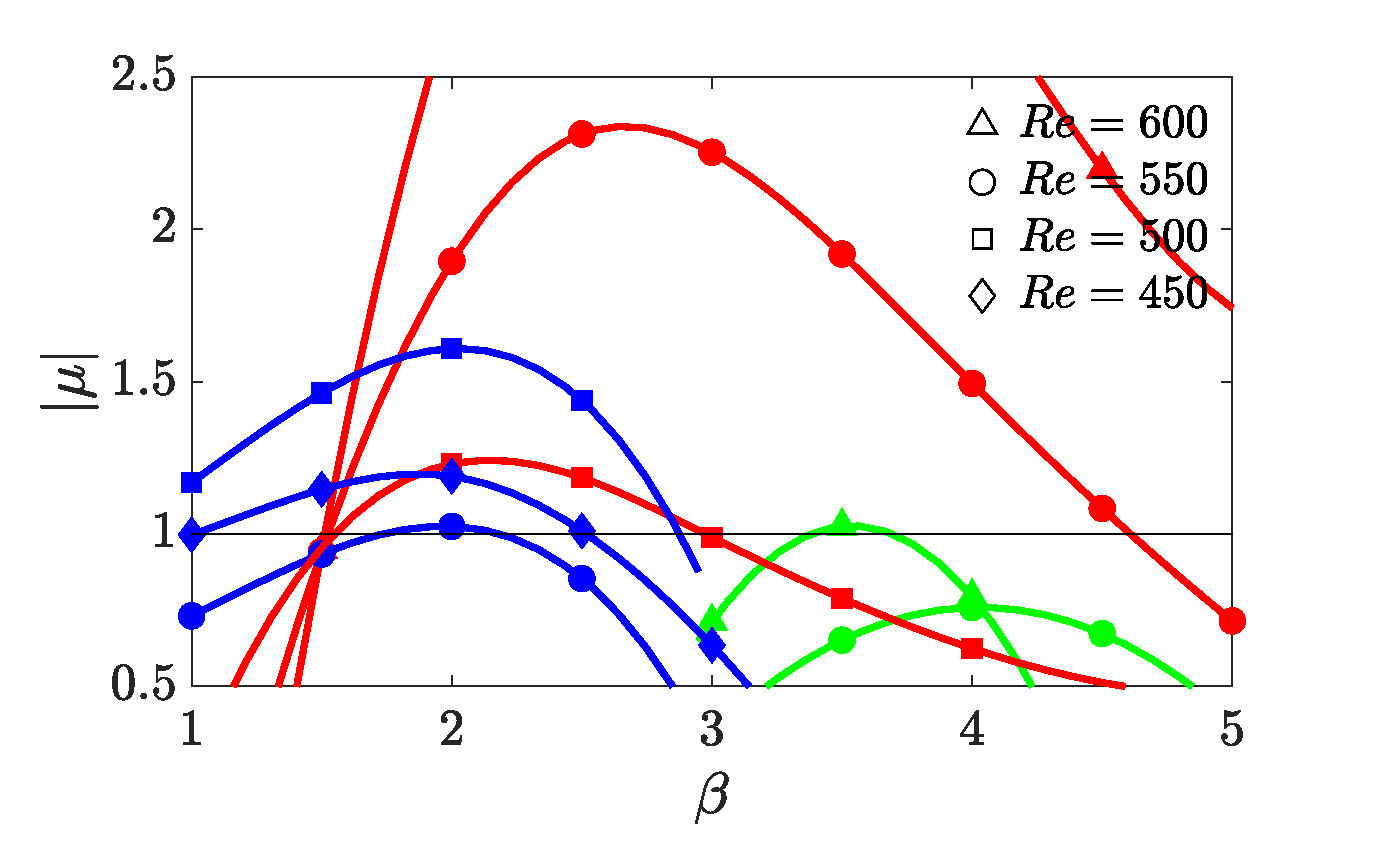
\includegraphics[width=0.49\textwidth]{./fig/AR5s/multipliers_AR5p5.eps}  
  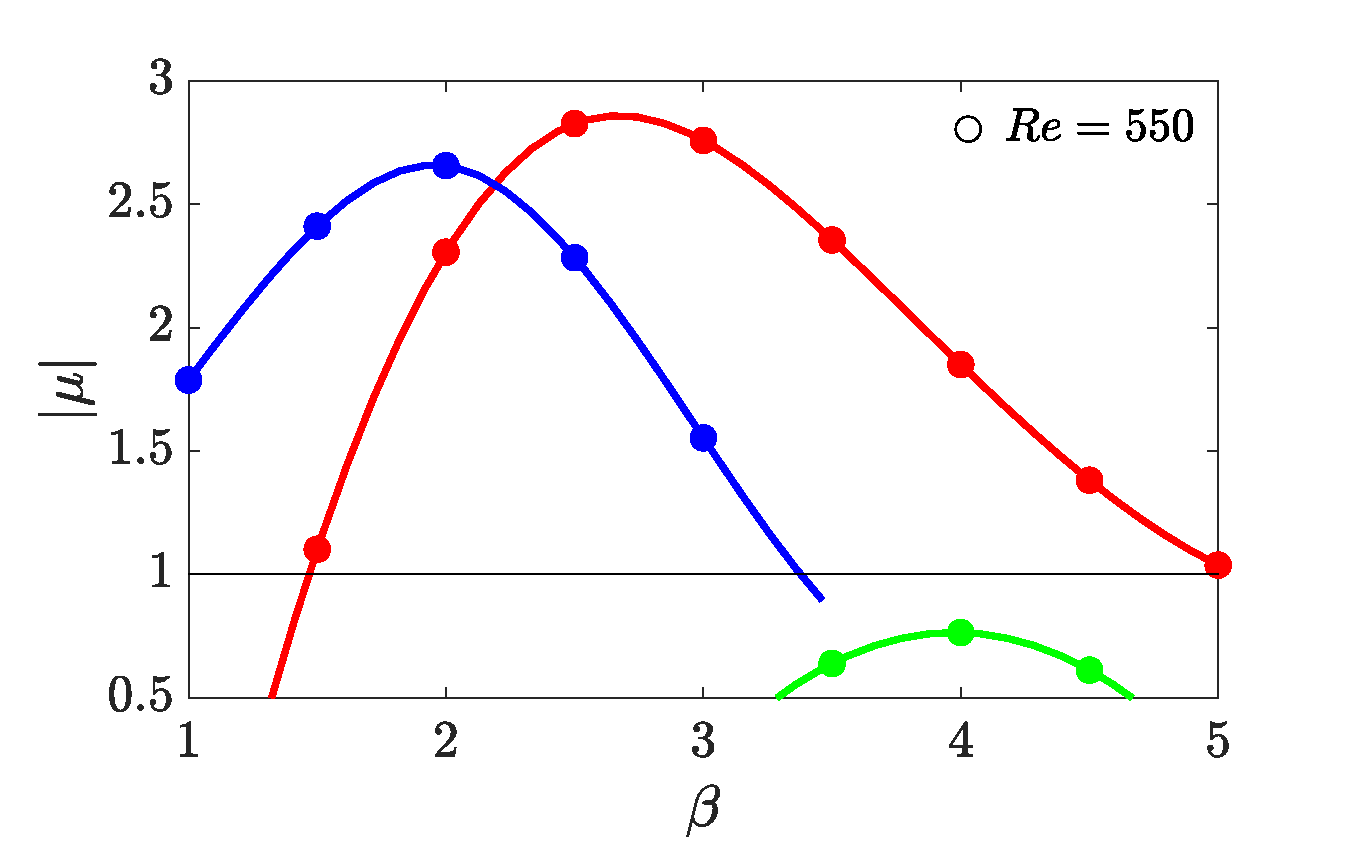
\includegraphics[width=0.49\textwidth]{./fig/AR5s/multipliers_AR5p75.eps} 
  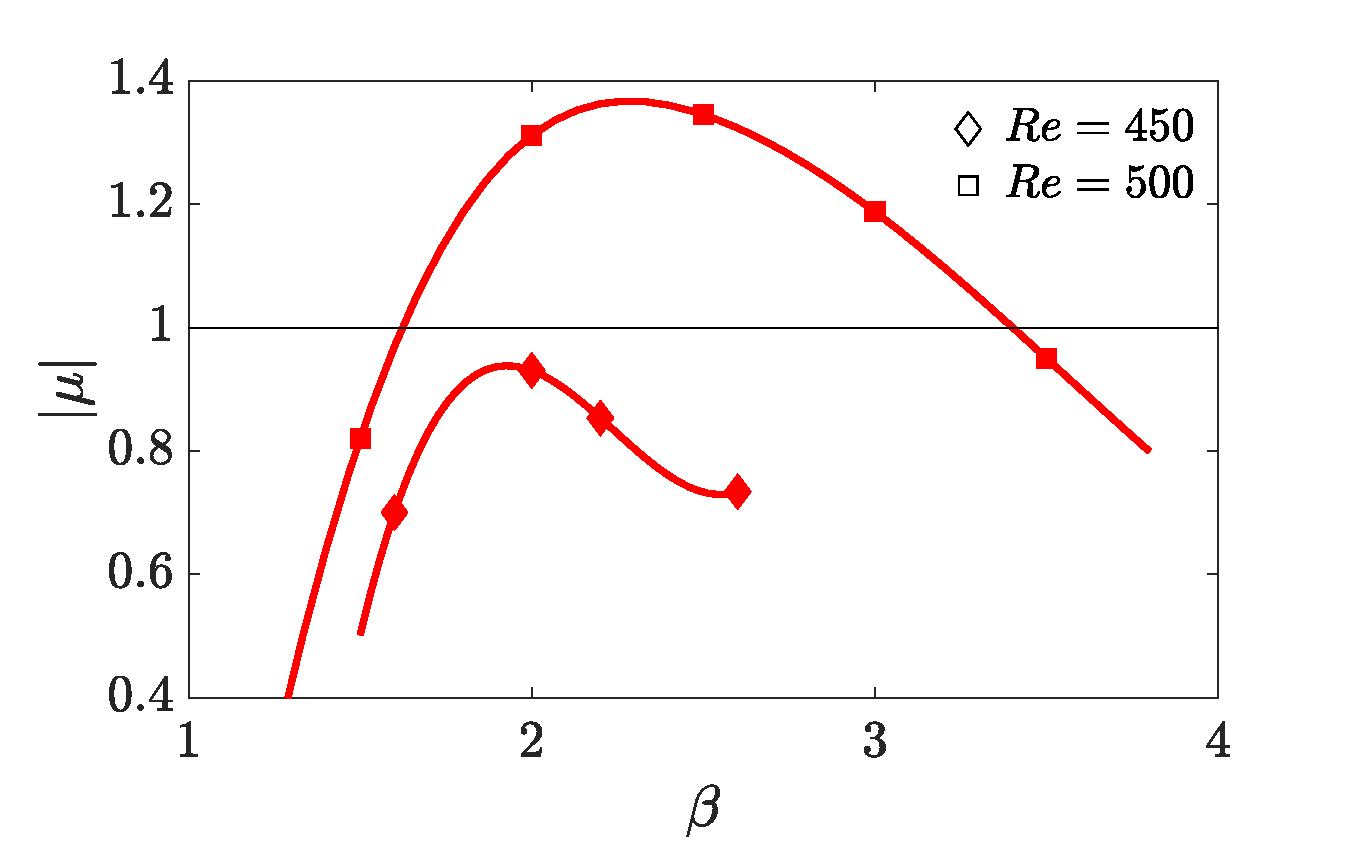
\includegraphics[width=0.49\textwidth]{./fig/AR7s/multipliers_AR6.eps}  
  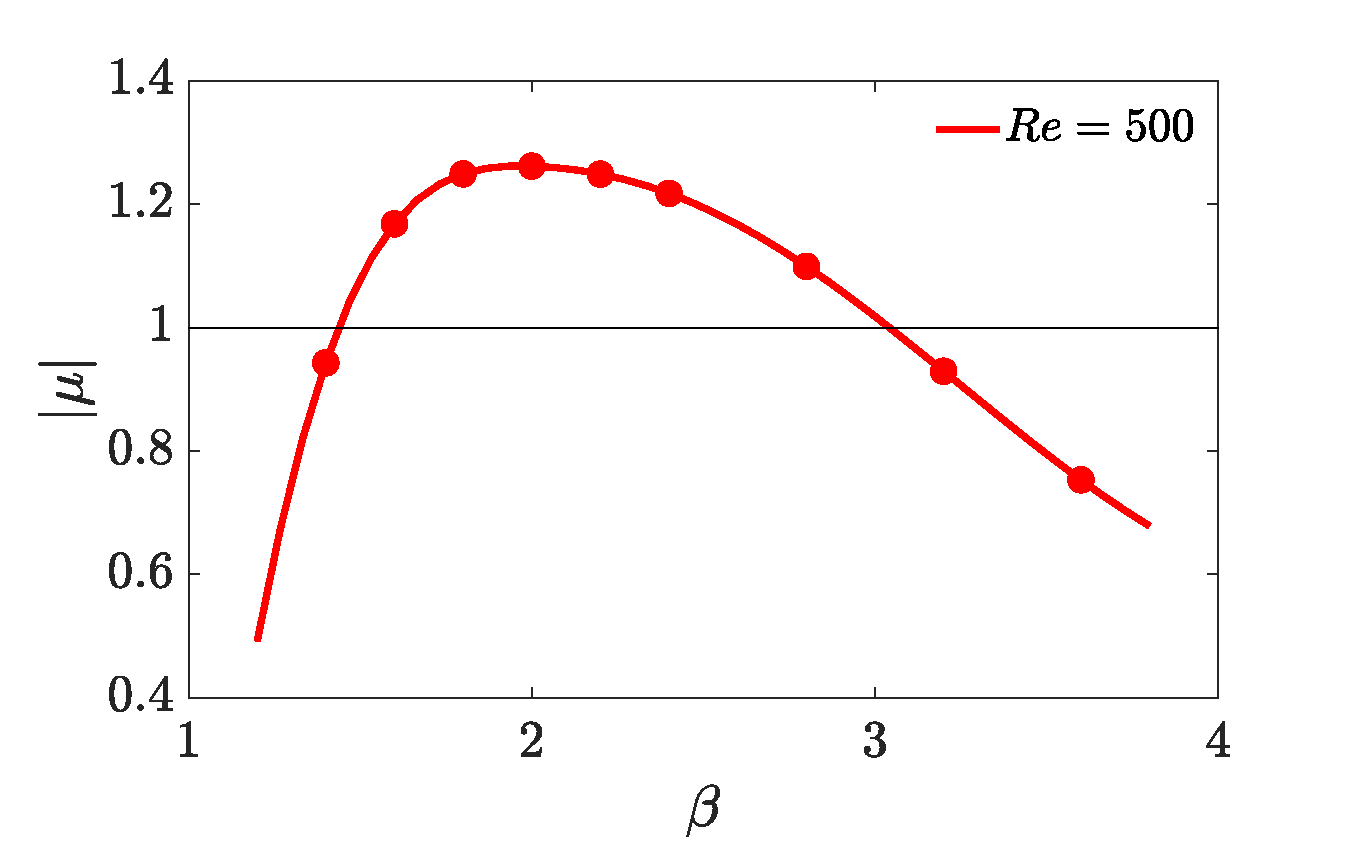
\includegraphics[width=0.49\textwidth]{./fig/AR7s/multipliers_AR7.eps}
  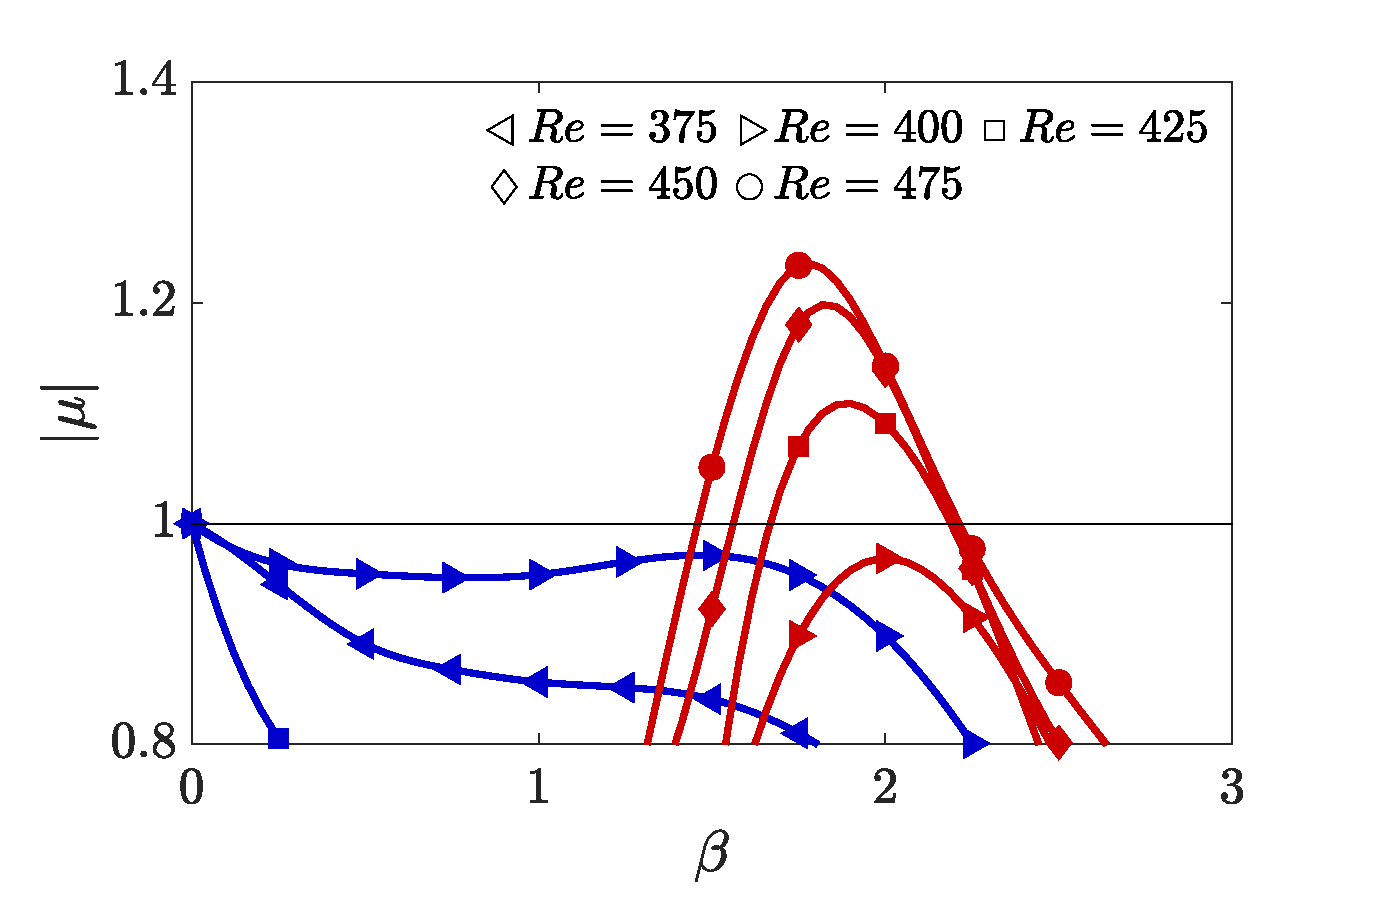
\includegraphics[width=0.49\textwidth]{./fig/AR9s/multipliers.eps}
  \caption{xx}
  \label{fig:multipliers_long}
\end{figure}

\begin{figure}
  \centering
  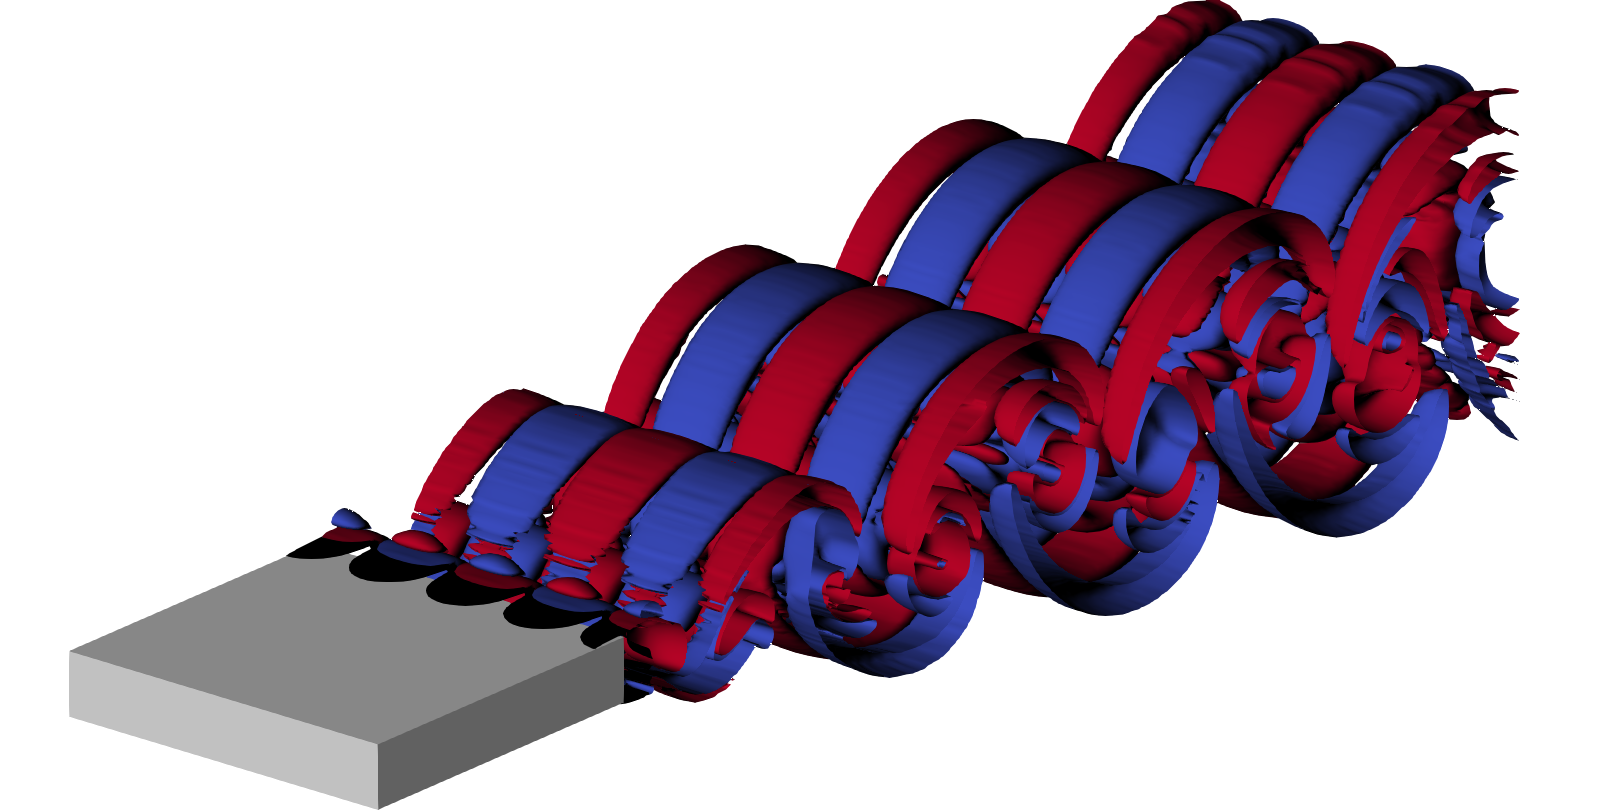
\includegraphics[width=0.49\textwidth]{./fig/AR5s/Floqetmode_beta_2_Re550_AR5p5_A.png}
  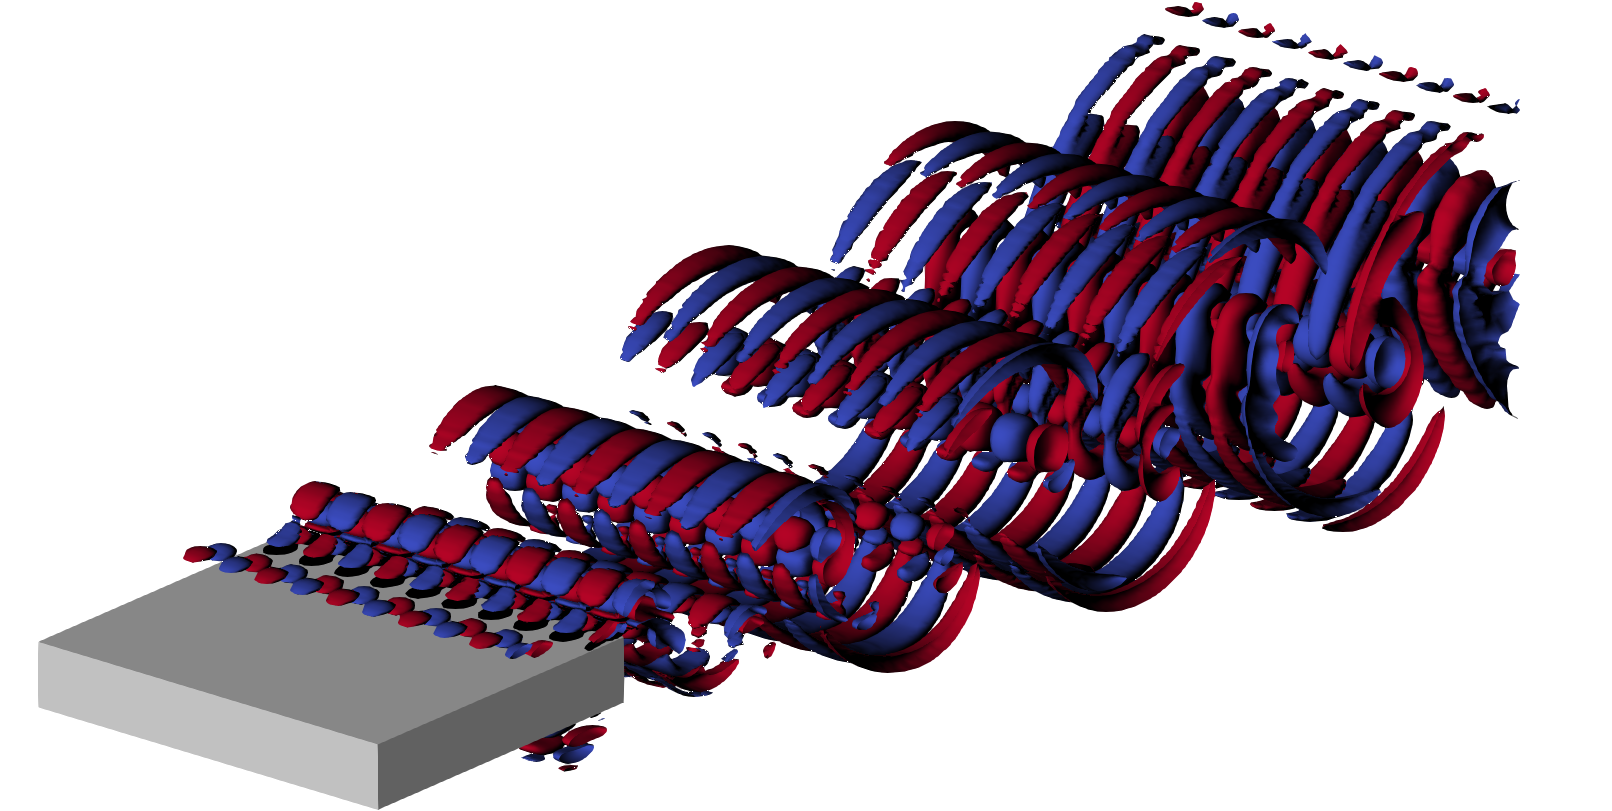
\includegraphics[width=0.49\textwidth]{./fig/AR5s/Floqetmode_beta_4p75_Re550_AR5p5_Ap.png}
  \includegraphics[width=0.49\textwidth]{./fig/AR5s/Floqetmode_beta_2_Re550_AR5p5_QS.png}   
  \includegraphics[width=0.49\textwidth]{./fig/AR9s/Floquet_AR9_Re450_beta2_modeQS.png}
  \caption{Three-dimensional reconstruction of the unstable modes for elongated bodies.}
  \label{fig:modes_long}
\end{figure}


\begin{figure}
  \centering
  \includegraphics[width=0.49\textwidth]{./fig/AR5p5/sens_1-200-1p25_5p5-500-2_modeA_75.png}
  \includegraphics[width=0.49\textwidth]{./fig/AR5p5/sens_1-200-1p25_5p5-500-2_modeA_100.png}
  \caption{Structural sensitivity for mode A at two different instants within the shedding period. Comparison between $\AR=5.5$ at $Re=500$ and $\beta=2$ and $\AR=1$ at $Re=200$ and $\beta=1.25$. For $\AR=5.5$ the base flow is governed by the TE vortex shedding. Though, the characteristic lengths of the wake vortex are rather different the topology of the structural sensitivity resembles in both cases at the two phases. This further suggests that in both cases the two unstable modes coincide.}
  \label{fig:sens_modeA}
\end{figure}

\begin{figure}
  \centering
  \includegraphics[width=0.49\textwidth]{./fig/AR5p5/Prod1_Re450_Re550_beta2.png}
  \includegraphics[width=0.49\textwidth]{./fig/AR5p5/Prod2_Re450_Re550_beta2.png}  
  \includegraphics[width=0.49\textwidth]{./fig/AR5p5/Mtrsp_Re450_Re550_beta2.png}
  \includegraphics[width=0.49\textwidth]{./fig/AR5p5/Ptrsp_Re450_Re550_beta2.png}
%  \includegraphics[width=0.49\textwidth]{./fig/AR5p5/Vtrsp_Re450_Re550_beta2.png}
%  \includegraphics[width=0.49\textwidth]{./fig/AR5p5/Diss_Re450_Re550_beta2.png}    
  \caption{Terms in the energy budget for $\AR=5.5$ and $Re=450$ (top) and $Re=550$ (bottom). In order the terms are $P_{uu}$, $P_{vv}$, $T_{m}$ and $T_p$}
  \label{fig:ener_bud}
\end{figure}

\begin{figure}
  \centering
%  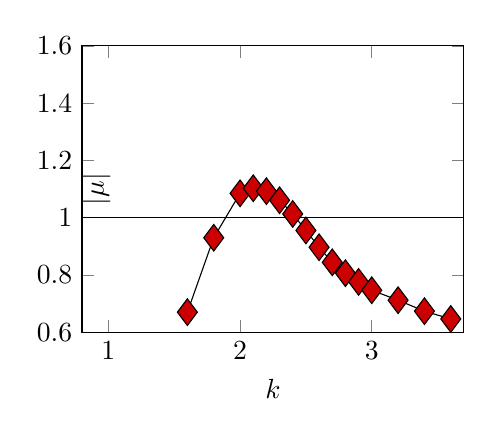
\begin{tikzpicture}



\begin{axis}[%
%width=4.3cm,
%height=3.5cm,
width=0.4\textwidth,
height=0.3\textwidth,
%width=0.2\textwidth,
%height=0.2\textwidth,
scale only axis,
%grid=both,
%axis lines=middle,
xmin=0.8,
xmax=3.7,
ymin=0.6,
ymax=1.6,
%xtick={2, 3, 4, 5, 6, 7, 8, 9, 10, 11},
%ytick={2, 2.5, 3, 3.5, 4, 4.5, 5, 5.5, 6, 6.5, 7},
%xlabel style={font=\color{white!15!black}},
xlabel={$k$},
ylabel={$|\mu|$},
ylabel style={at={(0.1,0.5)}},
%ymin=0,
%ymax=200,
axis background/.style={fill=white},
legend style={at={(0.99,0.85)}, anchor=east, legend cell align=left, align=left, fill=none, draw=none}
]


\addplot [color=black,solid,mark=diamond*,mark options={scale=2.4,black,fill=red!80!black}]
  table[row sep=crcr]{%
   %1.000000000000000   1.000070000000000 \\
  % 1.300000000000000   0.714343000000000 \\
   1.600000000000000   0.670046000000000 \\
   1.800000000000000   0.929885000000000 \\
   2.000000000000000   1.085060000000000 \\
   2.100000000000000   1.102700000000000 \\
   2.200000000000000   1.092560000000000 \\
   2.300000000000000   1.060710000000000 \\
   2.400000000000000   1.012990000000000 \\
   2.500000000000000   0.955412000000000 \\
   2.600000000000000   0.896718000000000 \\
   2.700000000000000   0.844065000000000 \\
   2.800000000000000   0.806200000000000 \\ 
   2.900000000000000   0.775755000000000 \\ 
   3.000000000000000   0.746579000000000 \\
   3.200000000000000   0.711819000000000 \\
   3.400000000000000   0.673520000000000 \\
   3.600000000000000   0.646376000000000 \\
   %4.000000000000000   0.562545000000000 \\
   %4.800000000000000   0.530527000000000 \\
   %5.000000000000000   0.524629000000000 \\
   %5.400000000000000   0.489231000000000 \\
   %5.800000000000000   0.468024000000000 \\
   %6.200000000000000   0.448075000000000 \\
};
%\addlegendentry{$Re=500$}

\addplot [color=black,solid,mark=,mark options={scale=1.4,black,fill=green!80!black}]
  table[row sep=crcr]{%
  0 1 \\
  5 1 \\
};





\end{axis}

\end{tikzpicture}%

%  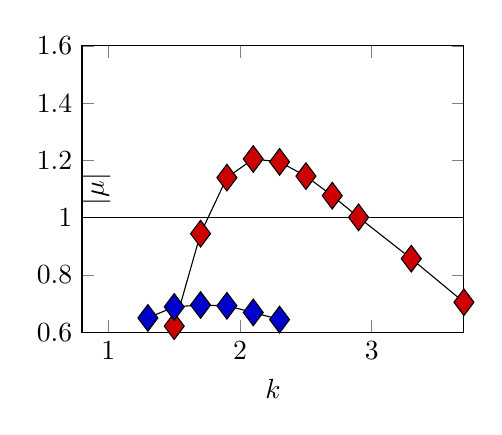
\begin{tikzpicture}



\begin{axis}[%
%width=4.3cm,
%height=3.5cm,
width=0.4\textwidth,
height=0.3\textwidth,
%width=0.2\textwidth,
%height=0.2\textwidth,
scale only axis,
%grid=both,
%axis lines=middle,
xmin=0.8,
xmax=3.7,
ymin=0.6,
ymax=1.6,
%xtick={2, 3, 4, 5, 6, 7, 8, 9, 10, 11},
%ytick={2, 2.5, 3, 3.5, 4, 4.5, 5, 5.5, 6, 6.5, 7},
%xlabel style={font=\color{white!15!black}},
xlabel={$k$},
ylabel={$|\mu|$},
ylabel style={at={(0.1,0.5)}},
%ymin=0,
%ymax=200,
axis background/.style={fill=white},
legend style={at={(0.99,0.85)}, anchor=east, legend cell align=left, align=left, fill=none, draw=none}
]


\addplot [color=black,solid,mark=diamond*,mark options={scale=2.4,black,fill=red!80!black}]
  table[row sep=crcr]{%
1.5 0.621431 \\
1.7 0.944234 \\
1.9 1.13979 \\
2.1 1.20487 \\
2.3 1.19477 \\
2.5 1.14503 \\
2.7 1.07689 \\
2.9 1.00122 \\
3.3 0.856827 \\
3.7 0.704753 \\
};
\addplot [color=black,solid,mark=diamond*,mark options={scale=2.4,black,fill=blue!80!black}]
  table[row sep=crcr]{%
1.3 0.650088 \\
1.5 0.688449 \\
1.7 0.695007 \\
1.9 0.692386 \\
2.1 0.669215 \\
2.3 0.644222 \\
};


%\addlegendentry{$Re=500$}

\addplot [color=black,solid,mark=,mark options={scale=2.4,black,fill=green!80!black}]
  table[row sep=crcr]{%
  0 1 \\
  5 1 \\
};





\end{axis}

\end{tikzpicture}%

%  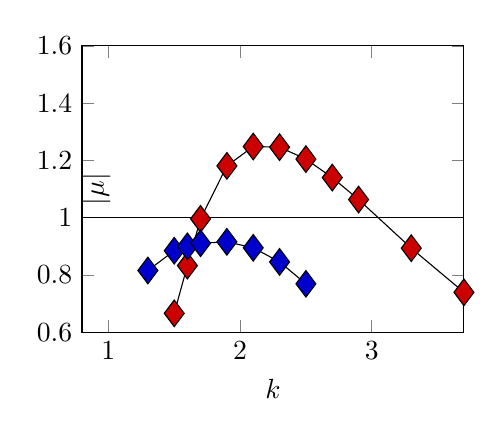
\begin{tikzpicture}



\begin{axis}[%
%width=4.3cm,
%height=3.5cm,
width=0.4\textwidth,
height=0.3\textwidth,
%width=0.2\textwidth,
%height=0.2\textwidth,
scale only axis,
%grid=both,
%axis lines=middle,
xmin=0.8,
xmax=3.7,
ymin=0.6,
ymax=1.6,
%xtick={2, 3, 4, 5, 6, 7, 8, 9, 10, 11},
%ytick={2, 2.5, 3, 3.5, 4, 4.5, 5, 5.5, 6, 6.5, 7},
%xlabel style={font=\color{white!15!black}},
xlabel={$k$},
ylabel={$|\mu|$},
ylabel style={at={(0.1,0.5)}},
%ymin=0,
%ymax=200,
axis background/.style={fill=white},
legend style={at={(0.99,0.85)}, anchor=east, legend cell align=left, align=left, fill=none, draw=none}
]


\addplot [color=black,solid,mark=diamond*,mark options={scale=2.4,black,fill=red!80!black}]
  table[row sep=crcr]{%
1.5 0.666004 \\
1.6 0.832646 \\
1.7 0.9958 \\
1.9 1.18082 \\
2.1 1.24832 \\
2.3 1.24618 \\
2.5 1.20433 \\
2.7 1.14004 \\
2.9 1.06321 \\
3.3 0.893504 \\
3.7 0.739385 \\
};
\addplot [color=black,solid,mark=diamond*,mark options={scale=2.4,black,fill=blue!80!black}]
  table[row sep=crcr]{%
1.3 0.815608 \\
1.5 0.884647 \\
1.6 0.899934 \\
1.7 0.910632 \\
1.9 0.915668 \\
2.1 0.89476 \\
2.3 0.845626 \\
2.5 0.769004 \\
%2.7 0.733247 \\
};


%\addlegendentry{$Re=500$}

\addplot [color=black,solid,mark=,mark options={scale=1.4,black,fill=green!80!black}]
  table[row sep=crcr]{%
  0 1 \\
  5 1 \\
};





\end{axis}

\end{tikzpicture}%
  
%  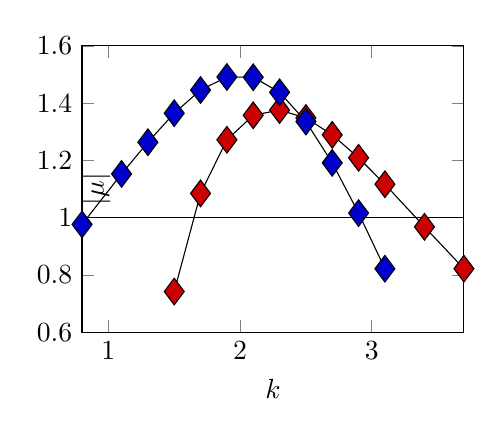
\begin{tikzpicture}



\begin{axis}[%
%width=4.3cm,
%height=3.5cm,
width=0.4\textwidth,
height=0.3\textwidth,
%width=0.2\textwidth,
%height=0.2\textwidth,
scale only axis,
%grid=both,
%axis lines=middle,
xmin=0.8,
xmax=3.7,
ymin=0.6,
ymax=1.6,
%xtick={2, 3, 4, 5, 6, 7, 8, 9, 10, 11},
%ytick={2, 2.5, 3, 3.5, 4, 4.5, 5, 5.5, 6, 6.5, 7},
%xlabel style={font=\color{white!15!black}},
xlabel={$k$},
ylabel={$|\mu|$},
ylabel style={at={(0.1,0.5)}},
%ymin=0,
%ymax=200,
axis background/.style={fill=white},
legend style={at={(0.99,0.85)}, anchor=east, legend cell align=left, align=left, fill=none, draw=none}
]


\addplot [color=black,solid,mark=diamond*,mark options={scale=2.4,black,fill=red!80!black}]
  table[row sep=crcr]{%
1.5 0.742066 \\
1.7 1.08482 \\
1.9 1.27188 \\
2.1 1.35744 \\
2.3 1.3757 \\
2.5 1.34816 \\
2.7 1.28908 \\
2.9 1.20902 \\
3.1 1.11666 \\
3.4 0.968 \\
3.7 0.821928 \\
};
\addplot [color=black,solid,mark=diamond*,mark options={scale=2.4,black,fill=blue!80!black}]
  table[row sep=crcr]{%
0.8 0.976452 \\
1.1 1.1528 \\
1.3 1.26332 \\
1.5 1.36481 \\
1.7 1.44557 \\
1.9 1.49116 \\
2.1 1.49023 \\
2.3 1.43771 \\
2.5 1.33553 \\
2.7 1.1913 \\
2.9 1.01607 \\
3.1 0.821755 \\
};


%\addlegendentry{$Re=500$}

\addplot [color=black,solid,mark=,mark options={scale=1.4,black,fill=green!80!black}]
  table[row sep=crcr]{%
  0 1 \\
  5 1 \\
};





\end{axis}

\end{tikzpicture}%

  \includegraphics[width=0.49\textwidth]{./fig/AR5s/multipliers_AR5.eps}
  \includegraphics[width=0.49\textwidth]{./fig/AR5s/multipliers_AR5p25.eps}  
  \includegraphics[width=0.49\textwidth]{./fig/AR5s/multipliers_AR5p5.eps}  
  \includegraphics[width=0.49\textwidth]{./fig/AR5s/multipliers_AR5p75.eps}      
  \vspace{0.1cm}
  \begin{tikzpicture}
  \draw (-10,2) -- (8,2);
  \end{tikzpicture}
  \vspace{0.1cm}
  \includegraphics[width=0.32\textwidth]{./fig/AR5s/Floqetmode_beta_2_Re550_AR5p5_A.png}
  \includegraphics[width=0.32\textwidth]{./fig/AR5s/Floqetmode_beta_2_Re550_AR5p5_QS.png} 
  \includegraphics[width=0.32\textwidth]{./fig/AR5s/Floqetmode_beta_4p75_Re550_AR5p5_Ap.png}
  \vspace{0.1cm}
  \begin{tikzpicture}
  \draw (-10,2) -- (8,2);
  \end{tikzpicture}
  \vspace{0.1cm}
  \includegraphics[width=0.49\textwidth]{./fig/AR5s/lambda2-AR55-Re450-3D.png}   
  \includegraphics[width=0.49\textwidth]{./fig/AR5s/lambda2-AR55-Re500-3D.png}     
  \caption{Top: Floquet multipliers for $\AR=5$ (top left), $\AR=5.25$ (top right), $\AR=5.5$ (bottom left) and $\AR=5.75$ (bottom right). The red symbols refer to mode $QS$. The blue symbols refer to mode $A$. The green symbols refer to mode $B$. Different symbols refer to different $Re$. Centre: Floquet modes associated with mode A (left), mode QS (centre) and mode $A'$ for $\AR=5.5$ and $Re=550$. Bottom: Results from the 3D DNS for $\AR=5.5$. Left: $Re=450$, right: $Re=500$. It is thus clear that mode A dominates at smaller $Re$, while once mode $QS$ becomes unstable it dominates. Mode $A'$ has the same symmetries of mode $A$ and is a synchronous mode. The difference is that its characteristic wavelength is much smaller, with $\beta_c \approx 4.5$. XX CHECK MODE GREEN FOR $AR=5.5$ and $Re=600$. POTREBBE ESSERE CHE SONO DUE MODI SEPARATI? XX}
  \label{fig:mult_AR5s}
\end{figure} 

%\section{Bodies with $6 \le \AR \le 8$}

\begin{itemize}
  \item For these $\AR$, the secondary flow instability is due to mode $QS$ that leads to a three-dimensional state. Interestingly, for these $\AR$ mode $A$ is not detected. This is consistent with the fact that for this range of $\AR$, at the intermediate $Re$, the flow is driven by the LE vortex shedding, that modifies the flow dynamics in the near-wake region where the triggering mechanism of mode $A$ takes place. 
\end{itemize}

\begin{figure}
  \centering
  \includegraphics[width=0.49\textwidth]{./fig/AR7s/multipliers_AR6.eps}  
  \includegraphics[width=0.49\textwidth]{./fig/AR7s/multipliers_AR7.eps}
  \includegraphics[width=0.49\textwidth]{./fig/AR7s/multipliers_AR7_b.eps}
  \includegraphics[width=0.7\textwidth]{./fig/AR7s/Floqetmode_beta_2p2_Re500_AR7.png}
  \caption{Floquet stability analysis for $\AR=6$ and $\AR=7$. Top: Floquet multipliers associated with the unstable branch. for $\AR=6$ (left) and $\AR=7$ (right). Centre: dependence of the real and imaginary parts of $\mu$ on $\beta$ for $\AR=7$. Bottom: three-dimensional reconstruction of the unstable Floquet mode for $\AR=7$. For these $\AR$s the secondary instability of the flow is due mode $QS$.}
  \label{fig:mult_AR7s}
\end{figure}

%\section{$\AR=9$}

\begin{figure}
  \centering
  \includegraphics[width=0.49\textwidth]{./fig/AR9s/Floquet_AR9_Re400_beta1p2_modeA.png}  
  \includegraphics[width=0.49\textwidth]{./fig/AR9s/Floquet_AR9_Re450_beta2_modeQS.png}
  \caption{Reconstruction of the Floquet modes for $\AR=9$. Left: mode $A$, $Re=400$, $\beta=1.2$. Right: mode $QS$, $Re=450$, $\beta=2$.}
  \label{fig:mult_AR9s}
\end{figure}

\begin{figure}
  \centering
  \includegraphics[width=0.49\textwidth]{./fig/AR5p5/sens_1-200-1p25_5p5-500-2_modeA_75.png}
  \includegraphics[width=0.49\textwidth]{./fig/AR5p5/sens_1-200-1p25_5p5-500-2_modeA_100.png}
  \caption{Structural sensitivity for mode A at two different instants within the shedding period. Comparison between $\AR=5.5$ at $Re=500$ and $\beta=2$ and $\AR=1$ at $Re=200$ and $\beta=1.25$. For $\AR=5.5$ the base flow is governed by the TE vortex shedding. Though, the characteristic lengths of the wake vortex are rather different the topology of the structural sensitivity resembles in both cases at the two phases. This further suggests that in both cases the two unstable modes coincide.}
  \label{fig:sens_modeA}
\end{figure} 
\fi
